\chapter{Simulation Results and Evaluation}
\label{ResultandEvaluation}

The simulations were done for line and grid scenarios, as well as for varying numbers of nodes and inter-node distances (4, 9, 16 nodes and 10, 50, 100 meters respectively). Furthermore, for each topology both objective functions OF0 and MRHOF were simulated. A total of 100 separate simulation runs were performed for each scenario setup. The simulation results are arranged in four parts according to the different simulation metrics, and each simulation metric is examined for the individual scenario setup.

\section{Default Route Discovery Time}
\label{default route}

The procedure for detecting the default route is described here. First Trickle sets the initial timer period t uniformly random in the range of $[128, 256)\:ms$\@. After the timer fired, the RPL root node (node~1 in the simulation) multicasts its first DIO message. Whichever node receives the message checks for the consistency between its own DODAG information and the one the DIO carries. Since it is the first DIO the receiver receives, it decides the DIO contains information about a new DODAG. Then the receiver adds the default route through the root node (node~1), updates its information to join the DODAG, and sets its own Trickle timer to the initial value. After its own timer fired, the receiver will forward the DIO, so the nodes which are more than one hop away from the root can add the default route as well.

The default route discovery time is presented by means of a CDF of the whole network. Figure~\ref{fig:dist10_montecarlo_cdf_hist} to Figure~\ref{fig:dist100_montecarlo_cdf_hist} show the CDF of default route discovery time for all three child nodes in the 4-node line scenario with different inter-node distances.

In Figure~\ref{fig:dist10_montecarlo_cdf_hist}, the inter-node distance is only 10~m, all three child nodes are one hop away from the root. In other words, all three child nodes will receive the first DIO from the root within the range of $[128, 256)\:ms$. Therefore the CDF shows a linear behavior until the default routes are found for all nodes.

\begin{figure}[htbp]
  \begin{center}
    \leavevmode
      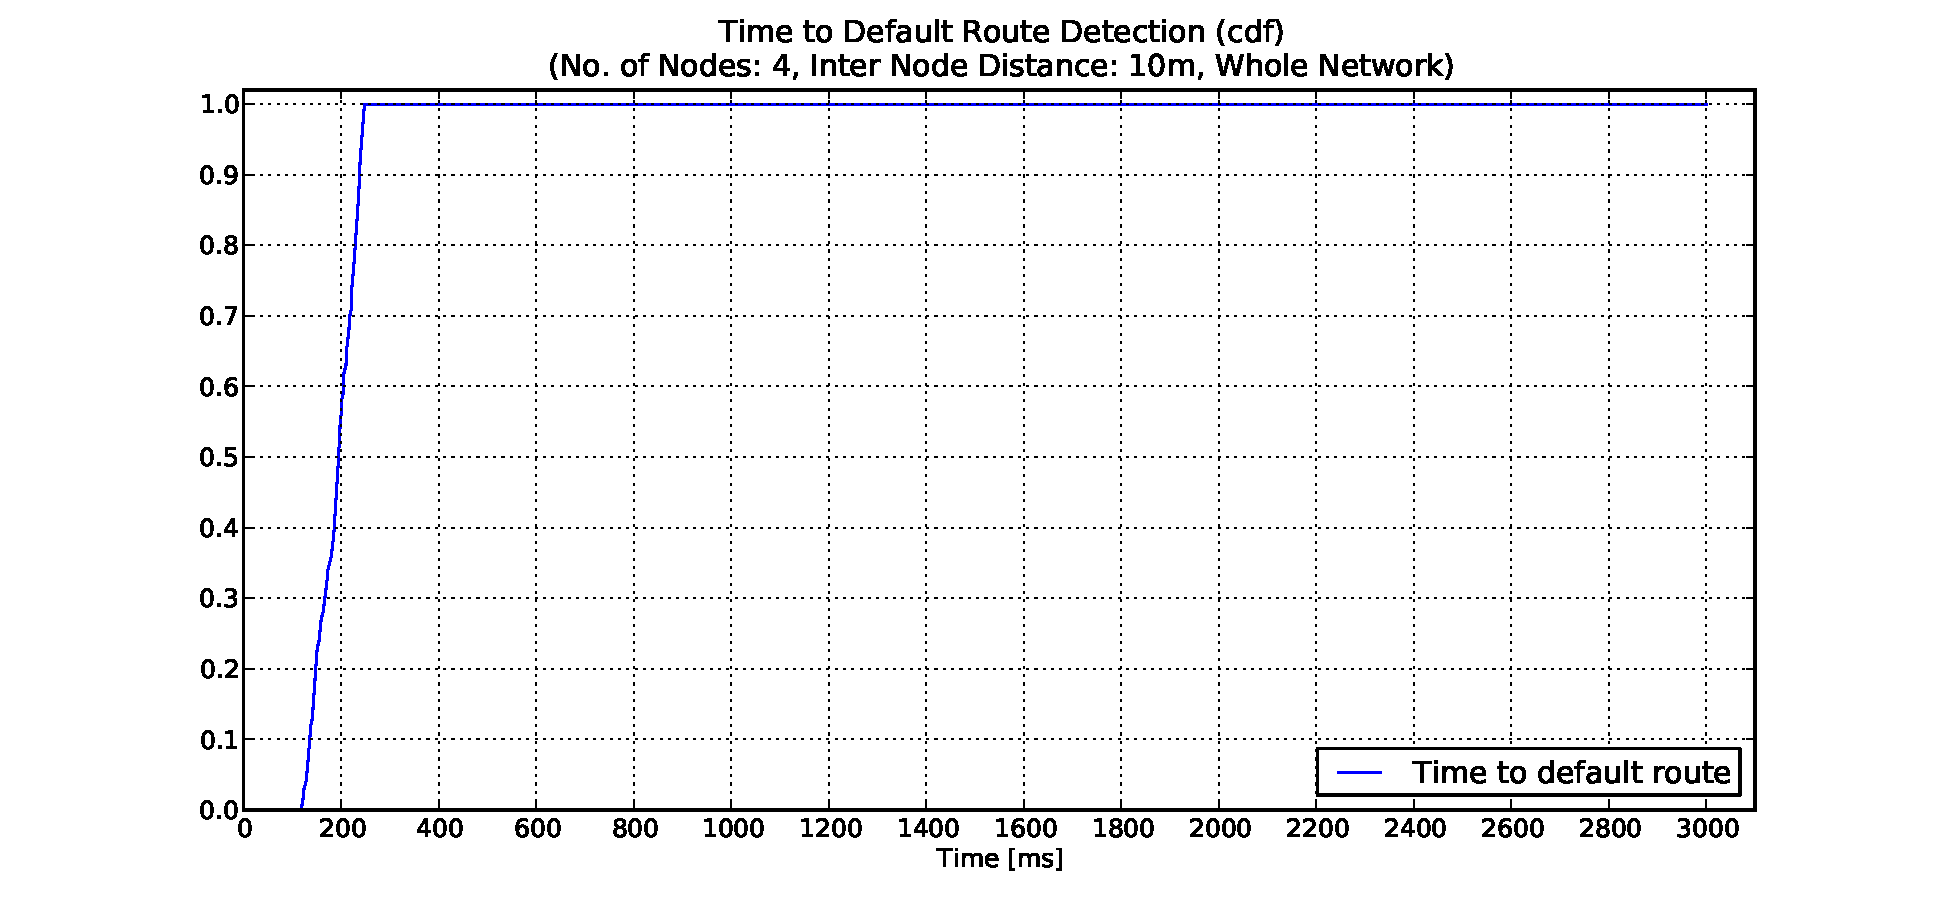
\includegraphics[scale=0.38]
      {Pics/results/4/MRHOF/line/dist10_montecarlo_cdf_hist.pdf}
   \caption{CDF of default route discovery time: 4-node line scenario with 10~m inter-node distance}
    \label{fig:dist10_montecarlo_cdf_hist}
  \end{center}
\end{figure}


In the case of Figure~\ref{fig:dist50_montecarlo_cdf_hist}, the distance between the root node and node 4 (the furthest node from the root) is 150~m which corresponds to a 39\% PRR. Therefore node 4 may be two hops away from the root. It is shown in Figure~\ref{fig:dist50_montecarlo_cdf_hist}, the linearity only goes up to around 70\%, and the CDF curve after that corresponds to the addition of two uniformly distributed random variables.

\begin{figure}[htbp]
  \begin{center}
    \leavevmode
      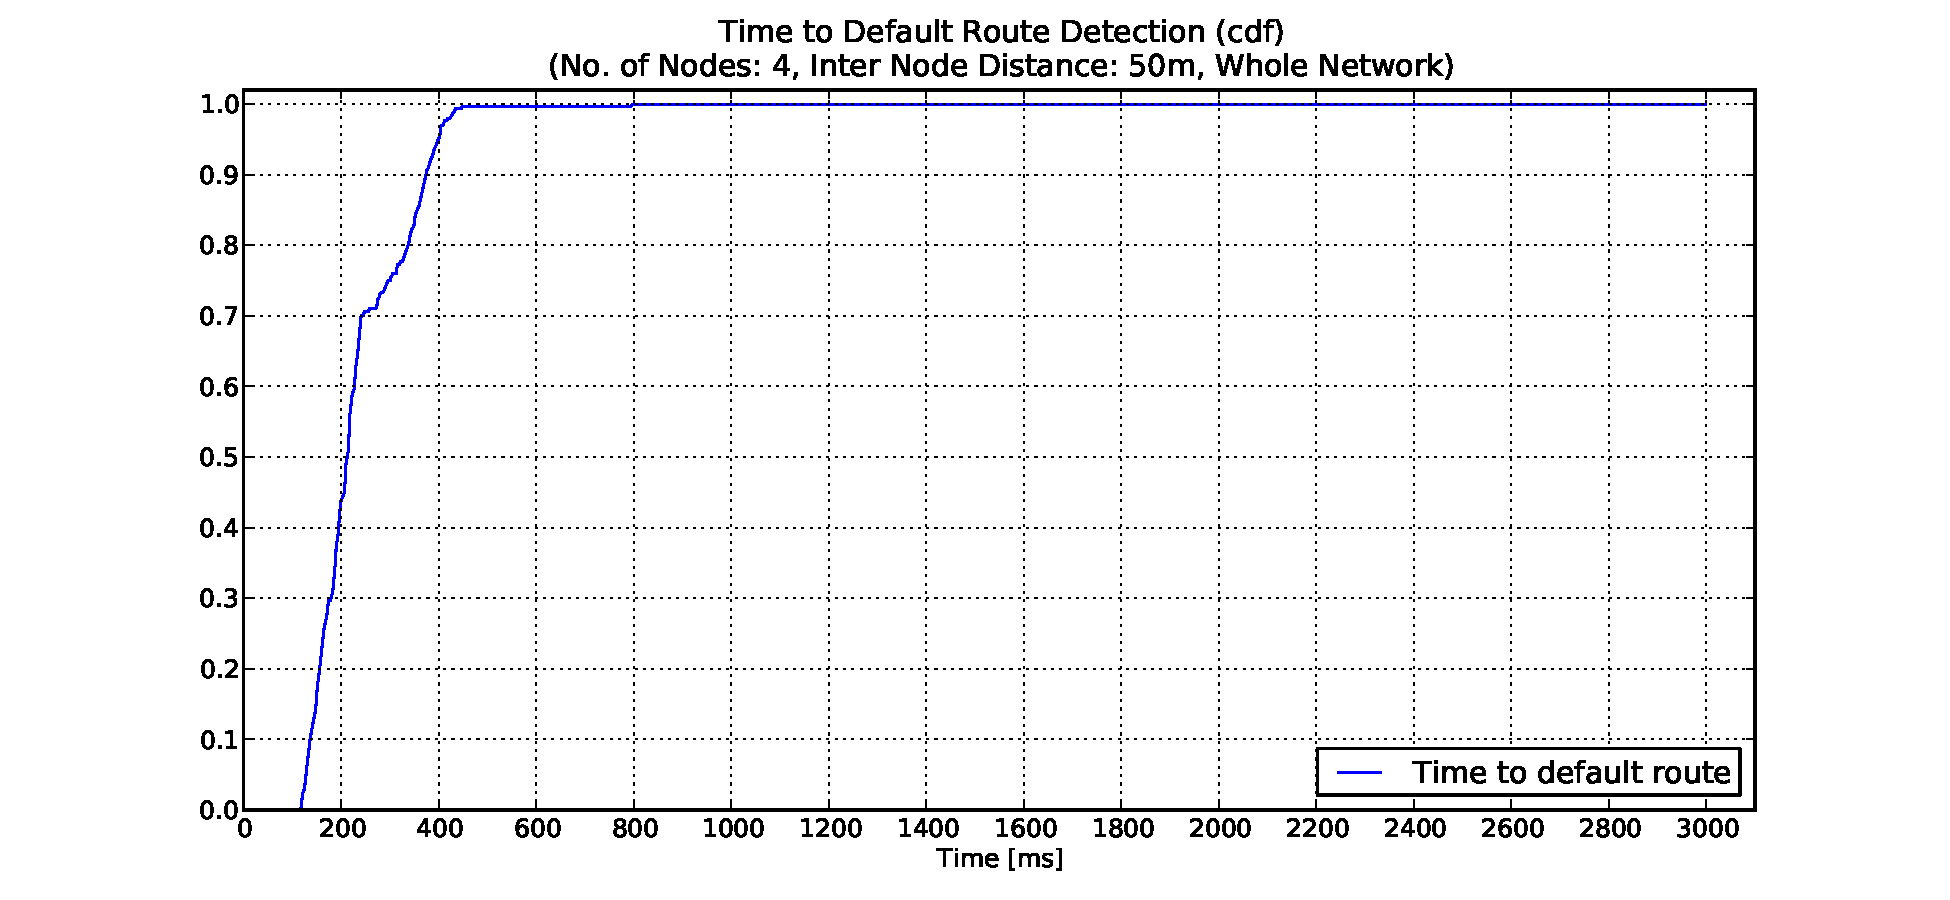
\includegraphics[scale=0.38]
      {Pics/results/4/MRHOF/line/dist50_montecarlo_cdf_hist.pdf}
   \caption{CDF of default route discovery time: 4-node line scenario with 50~m inter-node distance}
    \label{fig:dist50_montecarlo_cdf_hist}
  \end{center}
   \vspace{-20pt}
\end{figure}

The effect can be more precisely observed in Figure~\ref{fig:dist100_montecarlo_cdf_hist} where node 2 is one hop away from the root, node 3 is two hops away and node 4 is three hops away. The corresponding range of default route discovery time for node 2, 3 and 4 are $[128, 256)\:ms$, $[256, 512)\:ms$ and $[384, 768)\:ms$ respectively. Accordingly Figure~\ref{fig:dist100_montecarlo_cdf_hist} shows 3 phases in the CDF curve. The first phase (Time-axis from 128~ms to 256~ms) is linear. It demonstrates the CDF of the uniformly distributed default route discovery time for node 2. The second phase starts from 128~ms to 384~ms. The CDF of this phase corresponds to a triangle PDF which is the convolution of two uniform distributions PDFs. From 384~ms to 768~ms, a third uniform distribution is added. The CDF of this phase corresponds to an approximately bell shaped PDF.

% mab: $[128, 256)\:ms$, $[256, 512)\:ms$ and $[384, 768)\:ms$
% those values are not right! check them again!

\begin{figure}[htbp]
  \begin{center}
    \leavevmode
      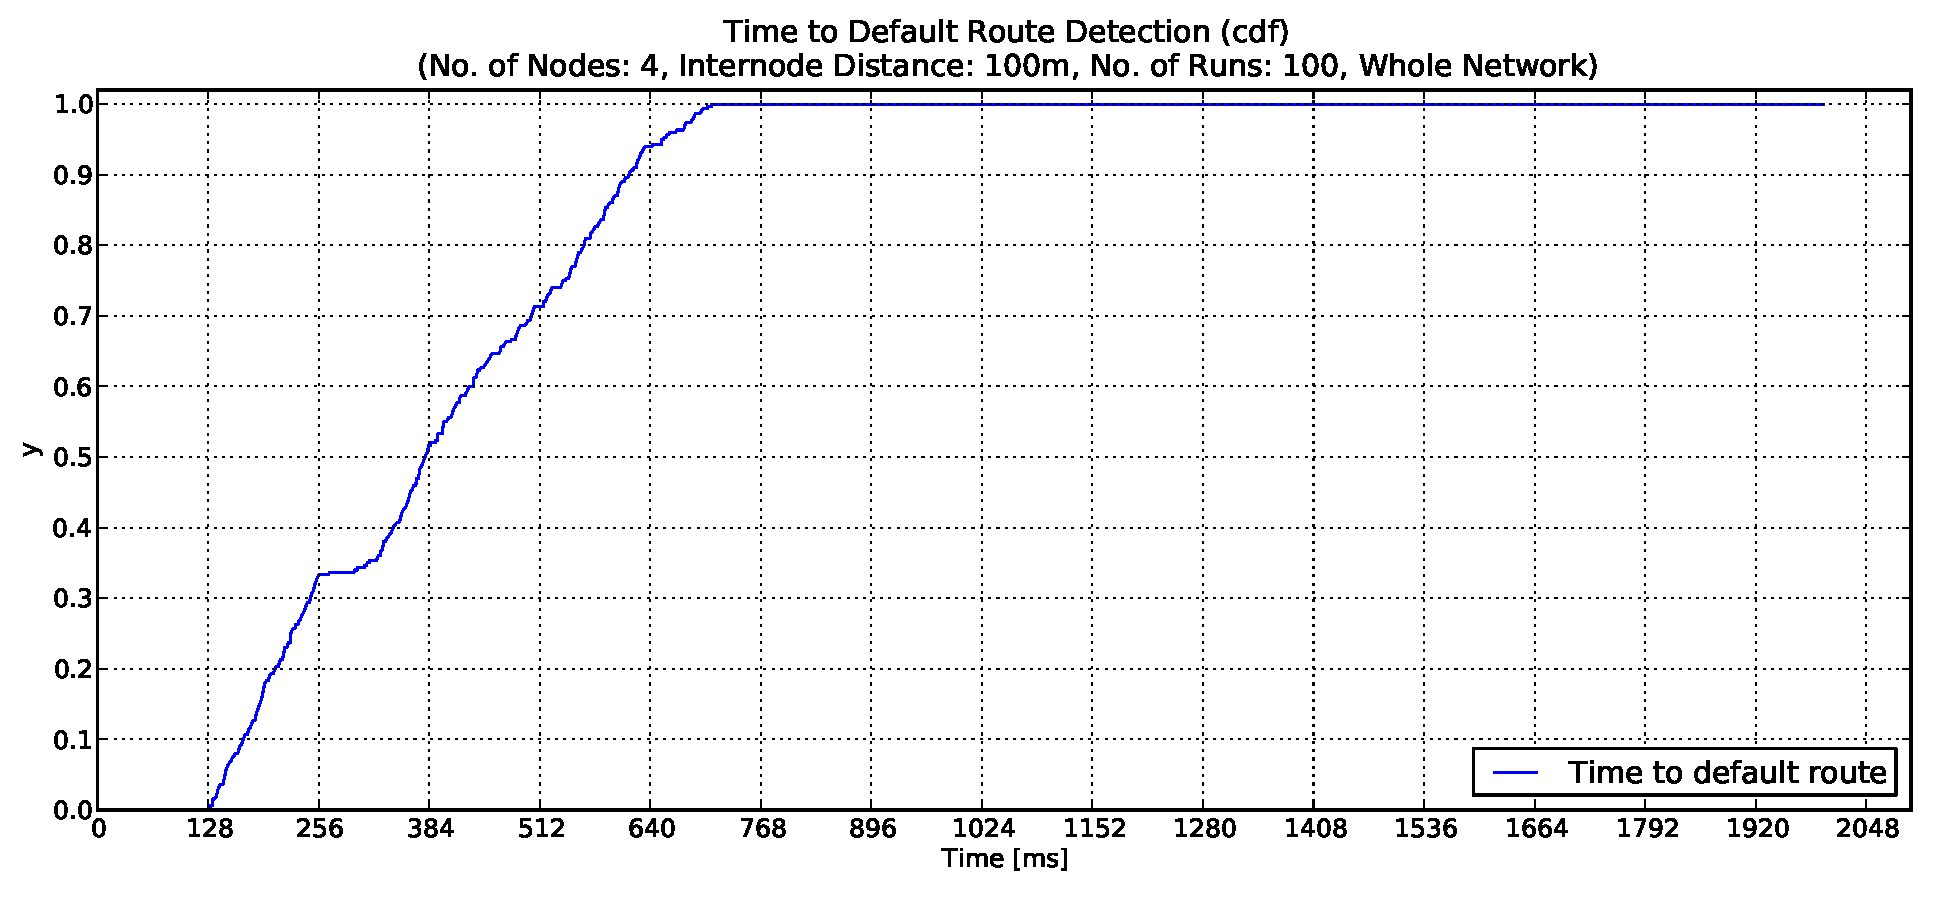
\includegraphics[scale=0.38]
      {Pics/results/4/MRHOF/line/dist100_montecarlo_cdf_hist.pdf}
   \caption{CDF of default route discovery time: 4-node line scenario with 100~m inter-node distance}
    \label{fig:dist100_montecarlo_cdf_hist}
  \end{center}
   \vspace{-20pt}
\end{figure}

The 95th percentiles of default route discovery time for line scenario and grid scenario with different node numbers and inter-node distances are shown in Table~\ref{table:95}. A 95th percentile is the value which 95\% of the observation results fall below. In this case it represents in 95\% of the simulation runs the lowest ranked node (largest hop distance from the root) is able to find the default routes within the 95th percentile. From the table, one can clearly see that the default route discovery time increases with the increase of distance and number of nodes. Additionally, all the 95th percentiles fall below $n*256\:ms$, where $n$ is the hop distance between the root and the node and 256~ms is the upperlimit of the initial time interval specified by Trickle timer $Imax$.

\begin{table}
\caption{The 95th percentile of default route discovery time}
\centering
    \begin{tabular}{ cc| c | c | c |} \cline{3-5}
     & & \multicolumn{3}{|c|}{inter-node Distance/m }\\ \cline{1-5}
     \multicolumn{1}{|c|}{Scenario} & No. of Nodes  & 10      & 50      & 100     \\  \hline
     \multicolumn{1}{|c|}{\multirow{3}{*}{Line}} &
    % \multicolumn{1}{|c|}{}      & 10      & 50      & 100     \\  \cline{2-5}
     \multicolumn{1}{|c|}{4}  & 250~ms  & 448~ms  & 650~ms  \\  \cline{2-5}
     \multicolumn{1}{|c|}{} & 9  & 256~ms  & 784~ms  & 1598~ms \\  \cline{2-5}
     \multicolumn{1}{|c|}{} & 16 & 320~ms  & 1363~ms & 2880~ms \\  \cline{1-5}
     \multicolumn{1}{|c|}{\multirow{3}{*}{Grid}} &
     \multicolumn{1}{|c|}{4}  & 256~ms  & 256~ms  & 380~ms  \\  \cline{2-5}
     \multicolumn{1}{|c|}{} & 9  & 250~ms  & 260~ms  & 576~ms  \\  \cline{2-5}
     \multicolumn{1}{|c|}{} & 16 & 250~ms  & 416~ms  & 736~ms  \\  \cline{1-5}  
    \end{tabular}
  \label{table:95}
\end{table}

The CDF histograms of default route discovery time for 9- and 16-node scenario setups can be found in Appendix~\ref{Appx:cdf}. 

% mab: Discussion of the table is missing!

\section{Control Message Overhead}
\label{ICMP}
The main advantage of using the Trickle algorithm is that it reduces the amount of control messages. In this section the control message (DIS, DIO and DAO) overhead in two 10-minute time intervals will be presented. The first 10-minute interval is taken right after all nodes are booted up. The second 10 minutes is from the 11th minute to the 20th. Since \texttt{UDPEcho} is configured to send messages with a period of 2 s, the simulation for the 4-node topology will only last for 600~ms.  Hence the control message overhead of the second interval will not be evaluated for the 4-node scenario.

Figure~\ref{fig:9_MRHOF_line_10_icmp} to Figure~\ref{fig:9_MRHOF_line_100_icmp} show the control message overhead  of the 9-node line scenario. One common thing that can be observed in these figures is, that node 1 always sends the least ICMP messages. It is because as root, node 1 does not sent any DIS and DAO messages. It only sends DIO messages.

In Figure~\ref{fig:9_MRHOF_line_10_icmp0}, the control message overhead is equally distributed among the child nodes since all of them are one hop away from the root. During the second 10-minute interval (Figure~\ref{fig:9_MRHOF_line_10_icmp1}), the amount of control messages is reduced from 21 (in the first 10 minutes) to 6 due to the effect of the Trickle timer. The simulation results show that under other scenario setups, the control message overheads during the second time intervals decrease in different degrees as compared to the ones in the first time intervals.

\begin{figure}[p]
  \begin{center}
    \leavevmode
    \subfloat[First 10 minutes]{\label{fig:9_MRHOF_line_10_icmp0}
      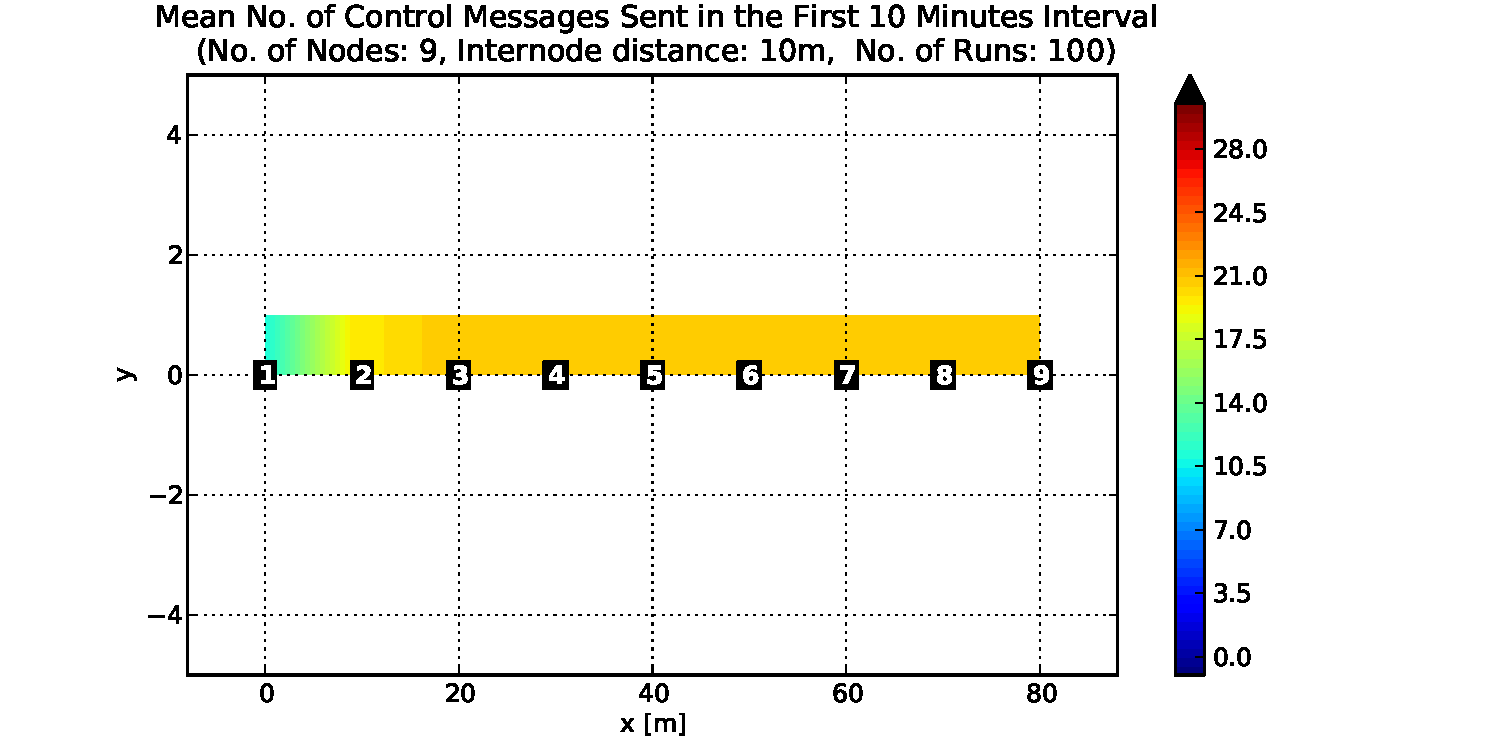
\includegraphics[trim=2cm 0cm 3cm 0cm, clip=true, scale=0.38] {Pics/results/9/MRHOF/line/dist10_montecarlo_contour_sent_ICMP_0.pdf}}
    \subfloat[Second 10 minutes]{\label{fig:9_MRHOF_line_10_icmp1}
       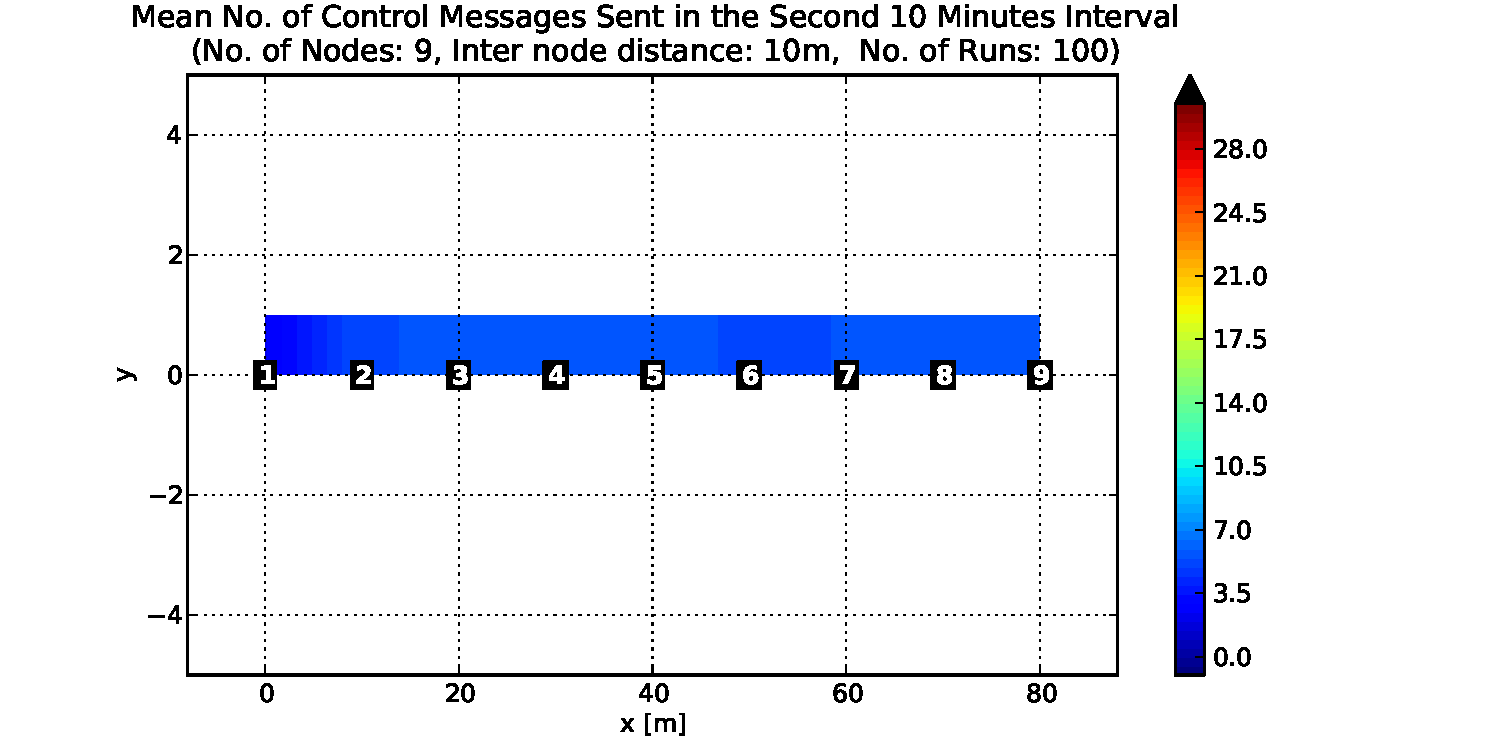
\includegraphics[trim=2cm 0cm 3cm 0cm, clip=true, scale=0.38] {Pics/results/9/MRHOF/line/dist10_montecarlo_contour_sent_ICMP_1.pdf}}
    \caption{Control message overhead: 9-node line scenario with 10~m inter-node distance}
    \label{fig:9_MRHOF_line_10_icmp}
  \end{center}
   \vspace{-20pt}
\end{figure}

\begin{figure}[p]
  \begin{center}
    \leavevmode
    \subfloat[First 10 minutes]{\label{fig:9_MRHOF_line_50_icmp0}
      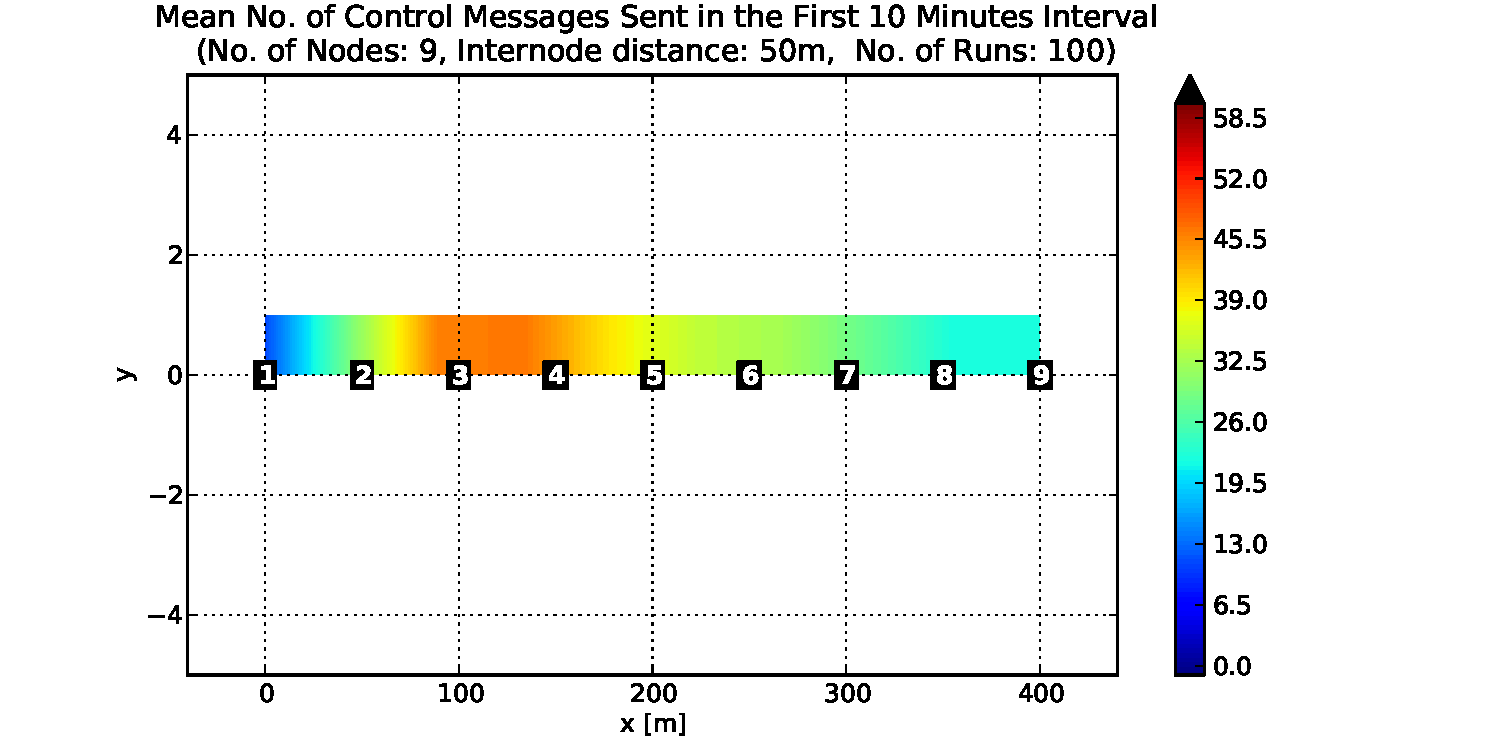
\includegraphics[trim=2cm 0cm 3cm 0cm, clip=true, scale=0.38]  {Pics/results/9/MRHOF/line/dist50_montecarlo_contour_sent_ICMP_0.pdf}}
    \subfloat[Second 10 minutes]{\label{fig:9_MRHOF_line_50_icmp1}
       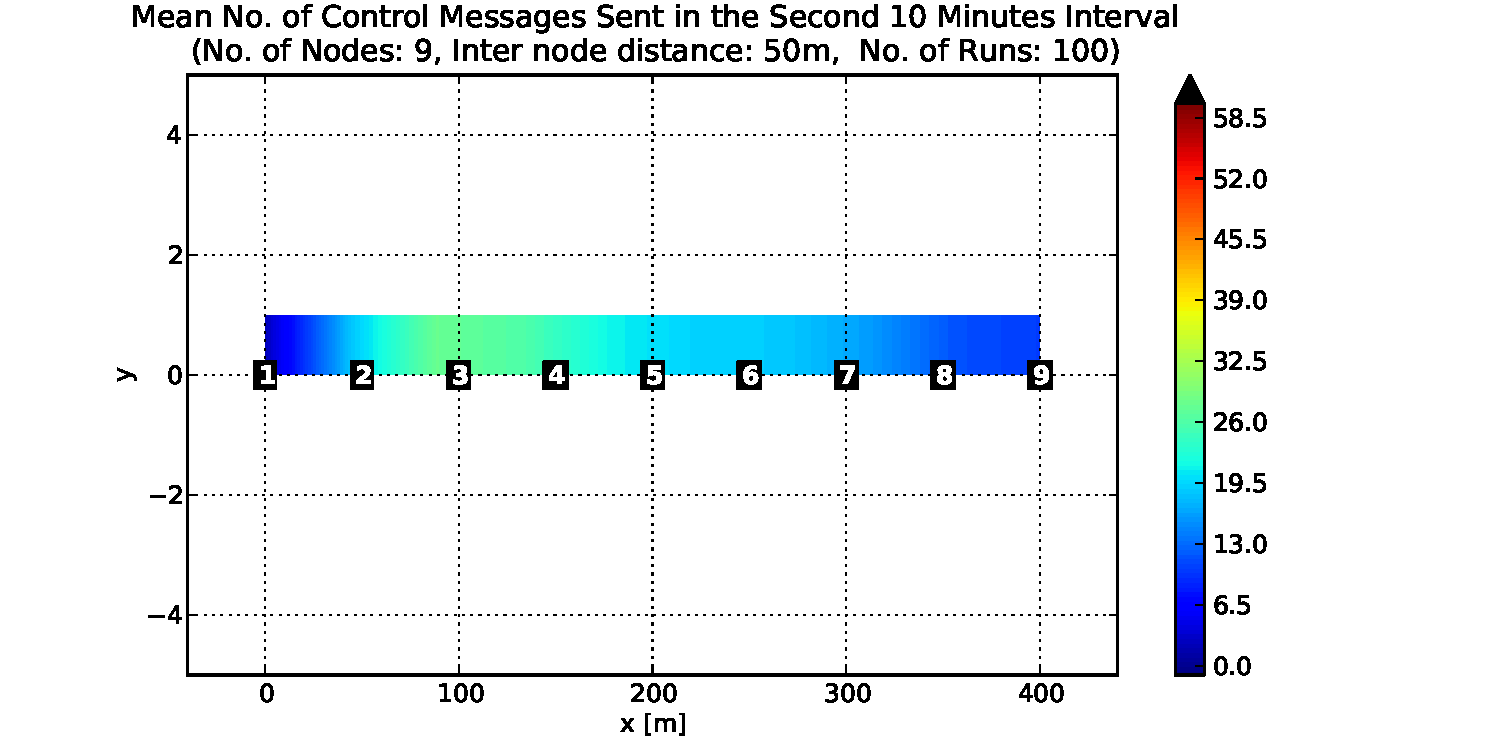
\includegraphics[trim=2cm 0cm 3cm 0cm, clip=true, scale=0.38]  {Pics/results/9/MRHOF/line/dist50_montecarlo_contour_sent_ICMP_1.pdf}}
    \caption{Control message overhead: 9-node line scenario with 50~m inter-node distance}
    \label{fig:9_MRHOF_line_50_icmp}
  \end{center}
    \vspace{-20pt}
\end{figure}

\begin{figure}[p]
  \begin{center}
    \leavevmode
    \subfloat[First 10 minutes]{\label{fig:9_MRHOF_line_100_icmp0}
      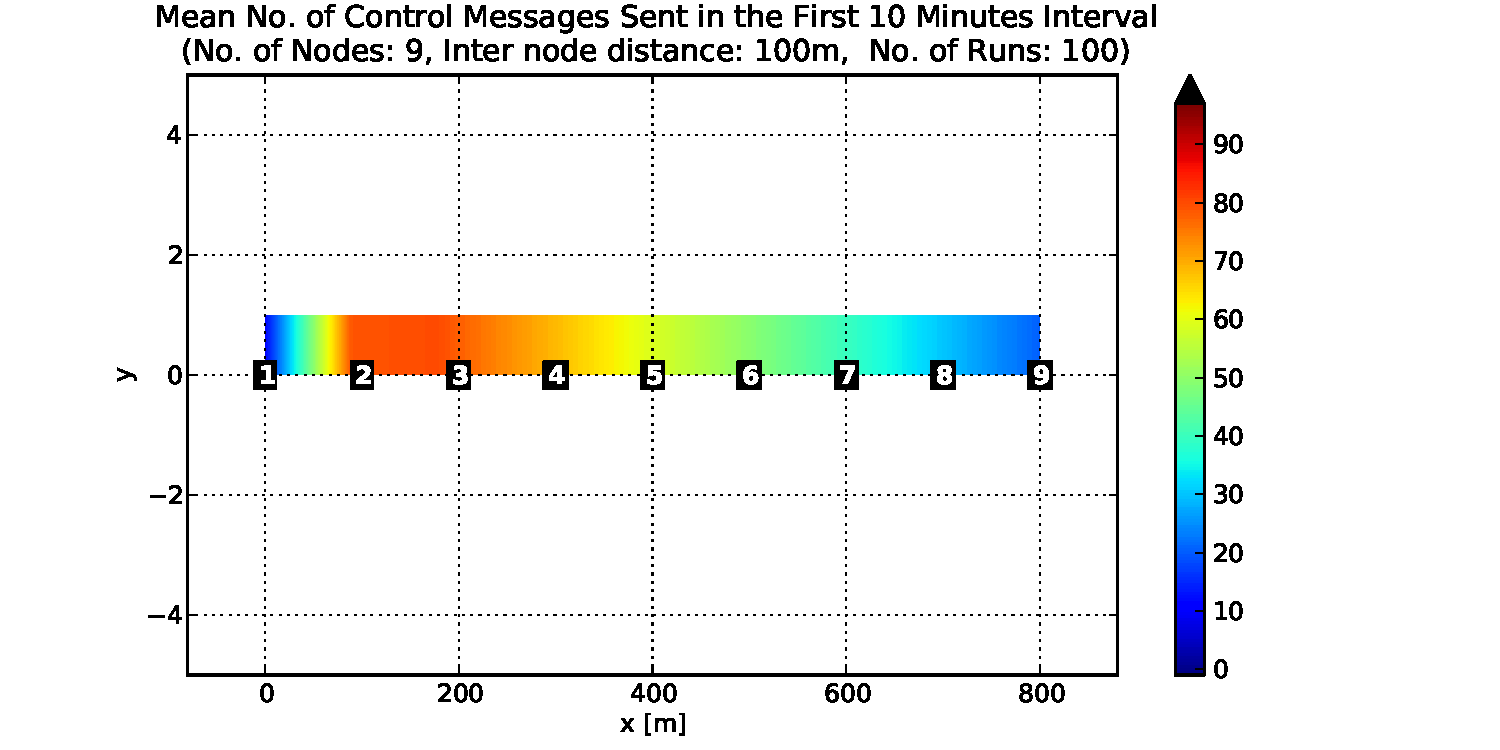
\includegraphics[trim=2cm 0cm 3cm 0cm, clip=true, scale=0.38] {Pics/results/9/MRHOF/line/dist100_montecarlo_contour_sent_ICMP_0}}
    \subfloat[Second 10 minutes]{\label{fig:9_MRHOF_line_100_icmp1}
       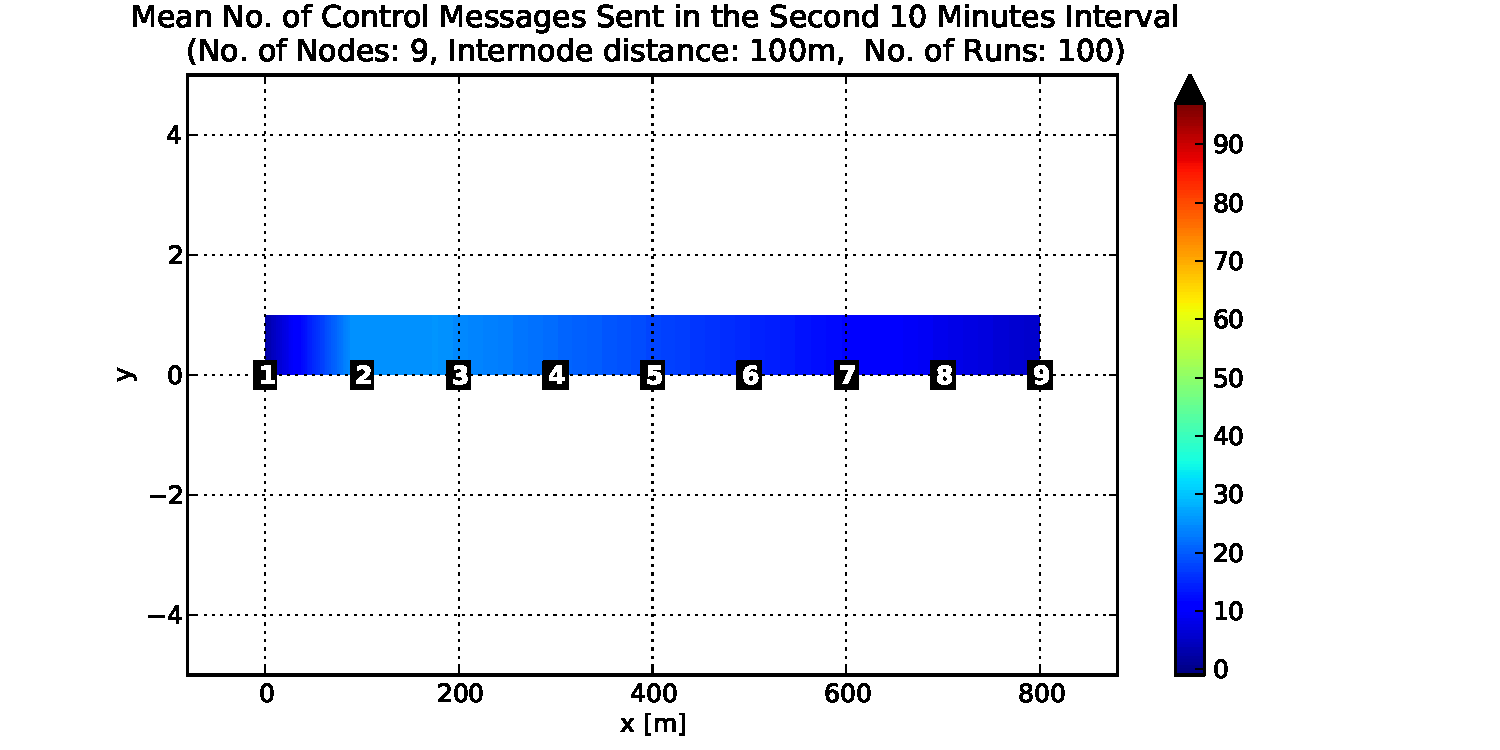
\includegraphics[trim=2cm 0cm 3cm 0cm, clip=true, scale=0.38] {Pics/results/9/MRHOF/line/dist100_montecarlo_contour_sent_ICMP_1}}
    \caption{Control message overhead: 9-node line scenario with 100~m inter-node distance}
    \label{fig:9_MRHOF_line_100_icmp}
  \end{center}
   \vspace{-20pt}
\end{figure}

As mentioned in Section~\ref{RPL:ICMP}, DAO is the control message which is used to discover and maintain the downward  route. DAO is sent upwards by a node and forwarded by the DAO parents until the message reaches the DODAG root. Therefore the nodes with lower rank have to forward DAOs which are originated from the higher rank nodes. Figure~\ref{fig:9_MRHOF_line_50_icmp0} and Figure~\ref{fig:9_MRHOF_line_100_icmp0} accurately demonstrate this behavior - the amount of control messages is high for node 3 and the number decreases along the downward route. During the second time interval, although the control message overhead is smaller compared to the first time interval, the same behavior can still be observed (Figure~\ref{fig:9_MRHOF_line_50_icmp1} and Figure~\ref{fig:9_MRHOF_line_100_icmp1}).

The control message behaviors of the 16-node line scenario and the grid scenarios are consistent with the results shown. The figures can be found in Appendix \ref{Appx:icmp}

\clearpage
\section{Packet Loss Rate}
\label{pl}

In the simulation a packet is considered to be lost when the echo packet is not received by the sender (in this case the root). 100 \texttt{UDPEcho} packets are sent from the root to each node in the network.

\subsection{Line Scenario}
\label{pl:line}

Figure~\ref{fig:pl_4_line_10} to Figure~\ref{fig:pl_4_line_100} show the mean packet loss rates for the 4-node line scenario with inter-node distances of 10, 50 or 100~m. The figures on the left show the results using OF0, and the right ones are the results using MRHOF. In Figure~\ref{fig:pl_9_line_10} to Figure~\ref{fig:pl_16_line_100}, the mean packet loss rates are presented in the same way for the 6- and 9-node line scenarios.

For the 4-node and 9-node line scenarios, the packet loss under the same setup shows no difference between OF0 and MRHOF. When the node number increases to 16, simulation with OF0 starts to exhibit a higher packet loss than MRHOF. In the 50 meters inter-node distance case (Figure~\ref{fig:16/OF0/line/dist50_montecarlo_contour_packetloss}), one can see a mean packet loss rate higher than 15\% for the most distant nodes. This result is caused by broken routes caused by low PRR and interferences between the root and the nodes in one or more runs out of the 100 runs. For most runs the loss rates are low. When the inter-node distance is increased to 100 meters, OF0 again presents a good case in terms of packet loss rate (Figure~\ref{fig:16/OF0/line/dist100_montecarlo_contour_packetloss}). Meanwhile, MRHOF continues to show stable results over all runs.
%\clearpage
\begin{figure}[p]
  \centering
    \leavevmode
    \subfloat[OF0]{\label{fig:4/OF0/line/dist10_montecarlo_contour_packetloss}
      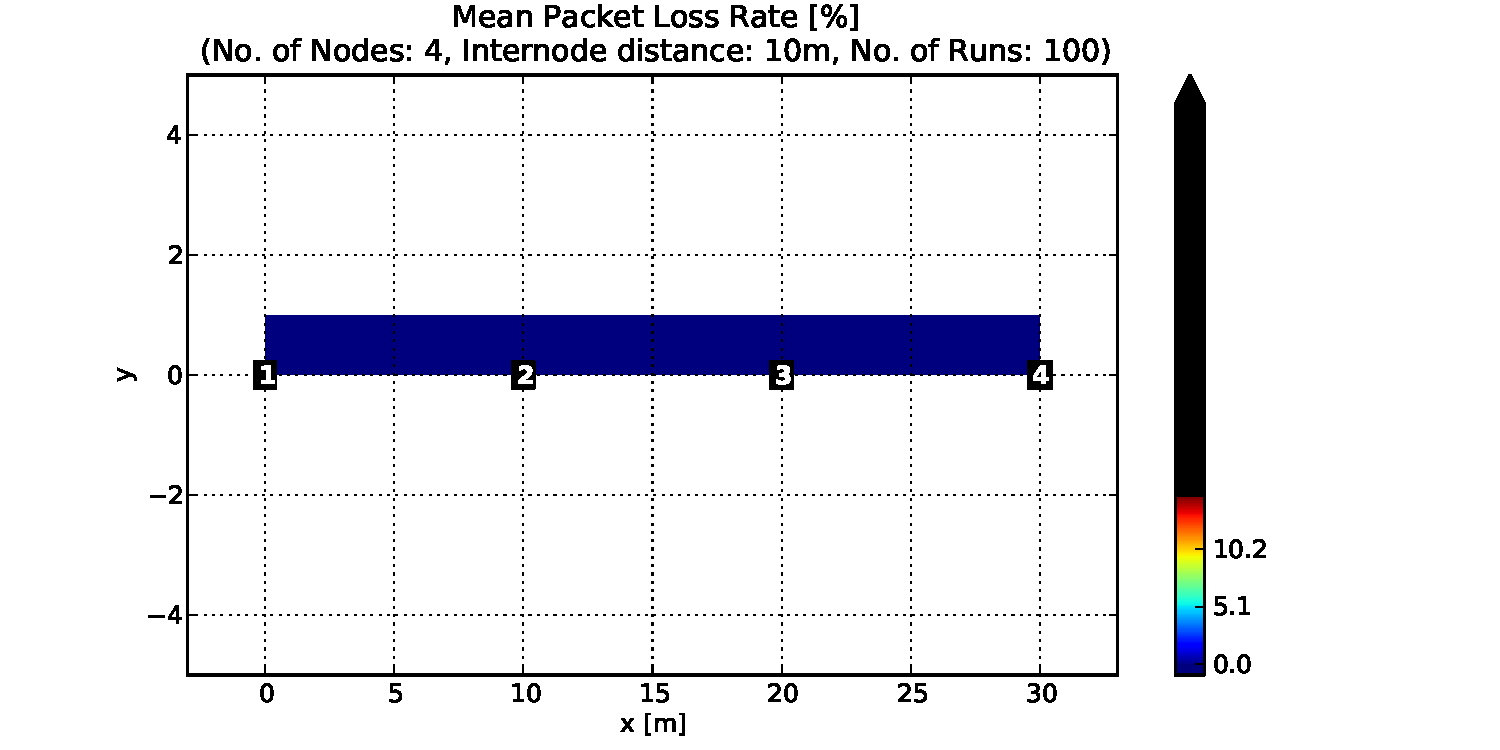
\includegraphics[trim=1.7cm 0cm 3cm 0cm, clip=true, scale=0.38]{Pics/results/4/OF0/line/dist10_montecarlo_contour_packetloss.pdf}}
    \subfloat[MRHOF]{\label{fig:4/MRHOF/line/dist10_montecarlo_contour_packetloss}
      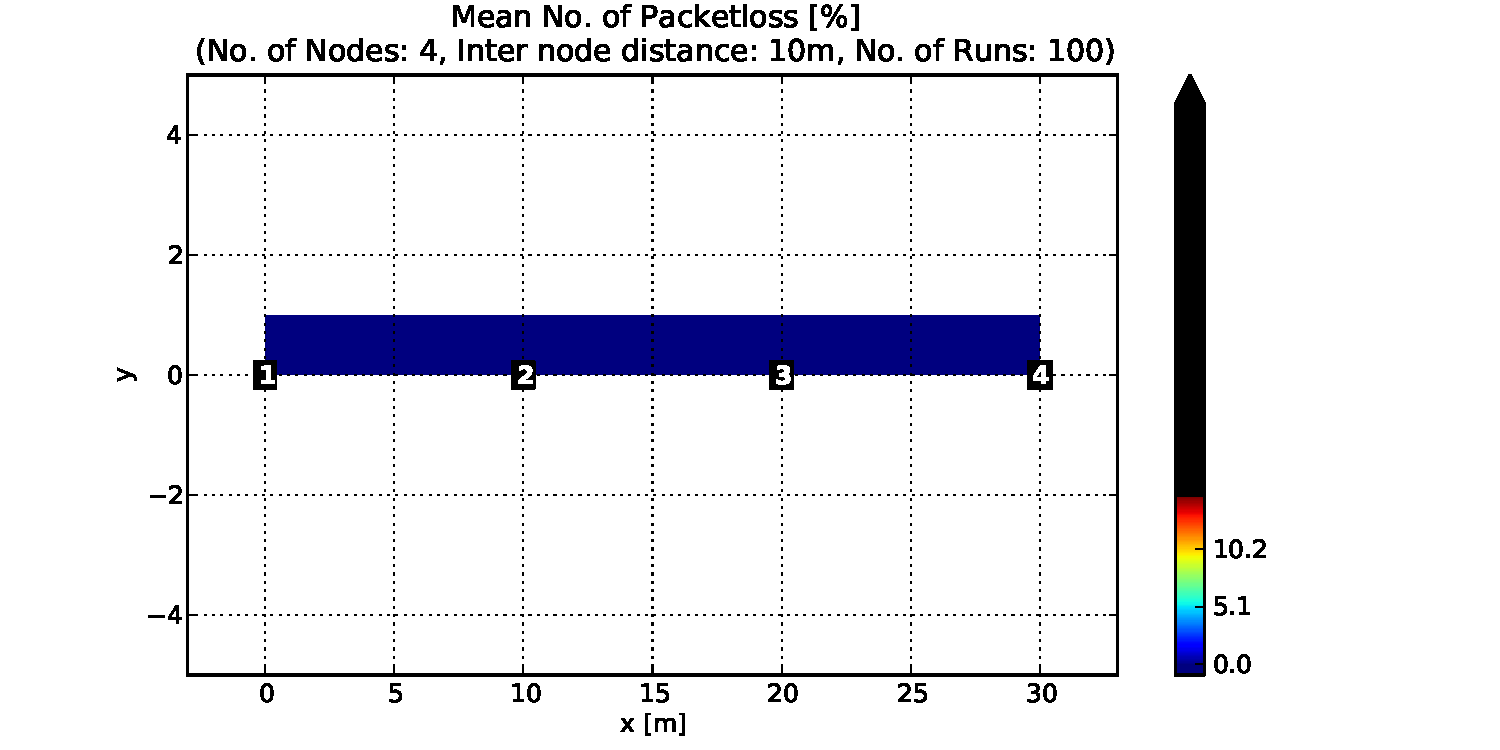
\includegraphics[trim=1.7cm 0cm 3cm 0cm, clip=true, scale=0.38]{Pics/results/4/MRHOF/line/dist10_montecarlo_contour_packetloss.pdf}}
   \caption{Mean packet loss rate: 4-node line scenario with 10~m inter-node distance}
   \label{fig:pl_4_line_10}
   \vspace{-20pt}
\end{figure}

\begin{figure}[p]
  \centering
    \leavevmode
    \subfloat[OF0]{\label{fig:4/OF0/line/dist50_montecarlo_contour_packetloss}
    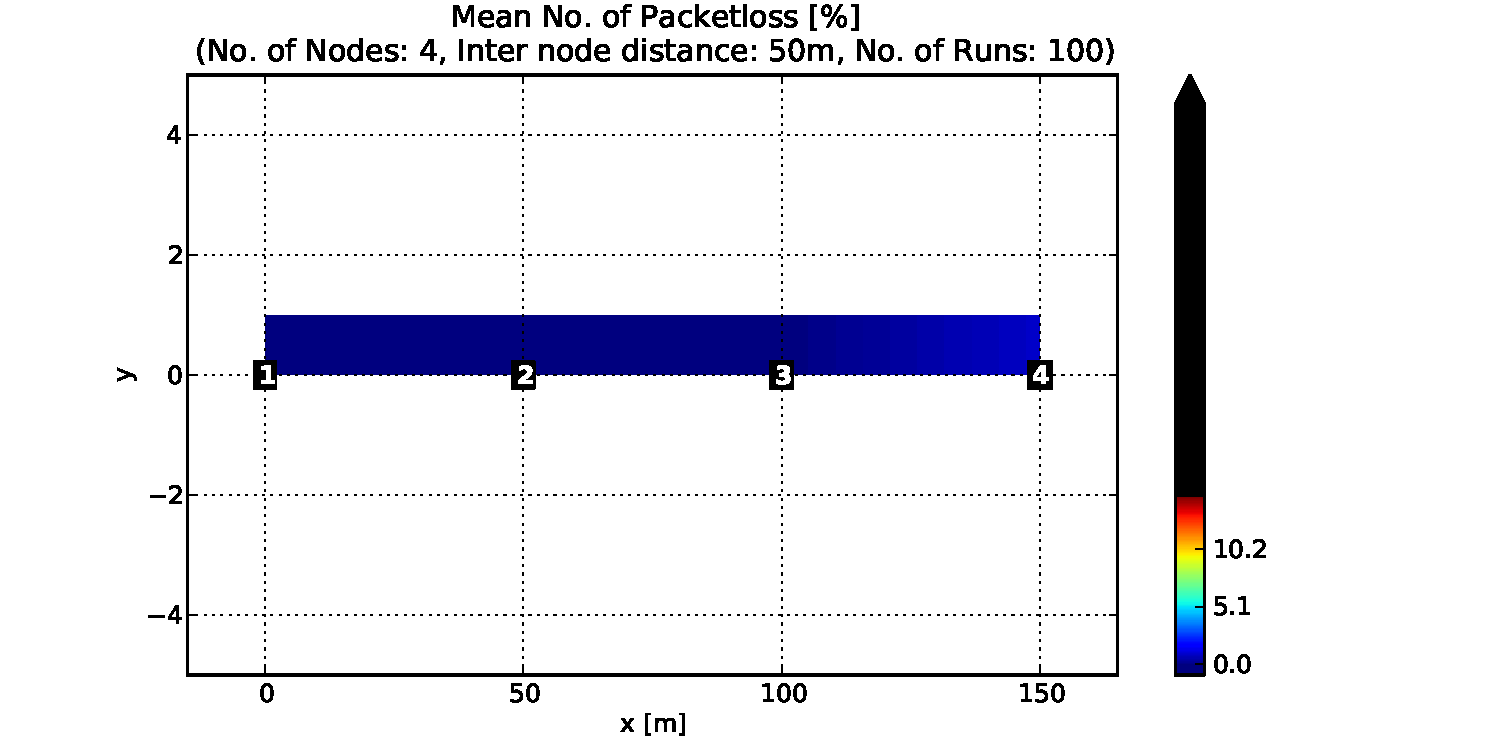
\includegraphics[trim=1.7cm 0cm 3cm 0cm, clip=true, scale=0.38]   {Pics/results/4/OF0/line/dist50_montecarlo_contour_packetloss.pdf}}
    \subfloat[MRHOF]{\label{fig:4/MRHOF/line/dist50_montecarlo_contour_packetloss}
      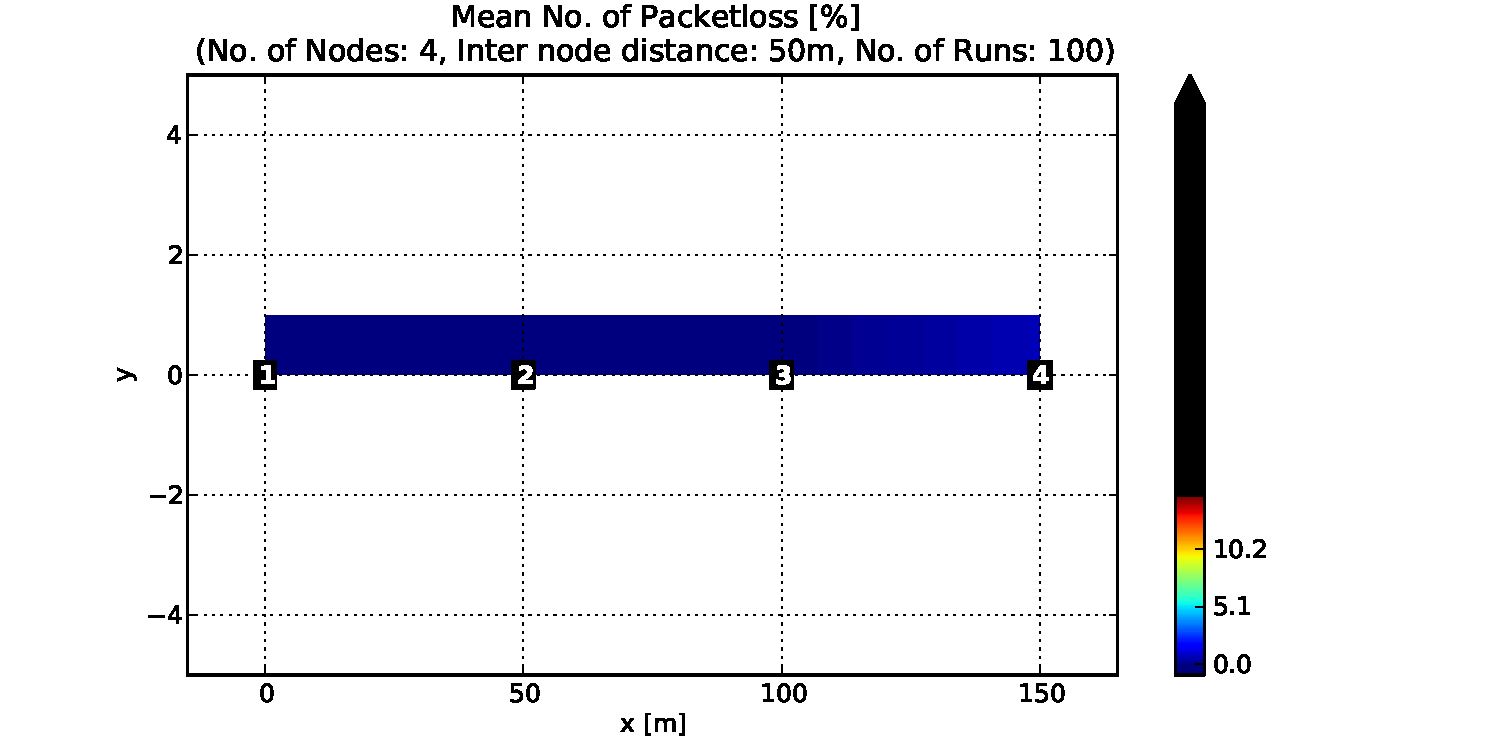
\includegraphics[trim=1.7cm 0cm 3cm 0cm, clip=true, scale=0.38]{Pics/results/4/MRHOF/line/dist50_montecarlo_contour_packetloss.pdf}}
   \caption{Mean packet loss rate: 4-node line scenario with 50~m inter-node distance}
   \label{fig:pl_4_line_50}
   \vspace{-20pt}
\end{figure}

\begin{figure}[p]
  \centering
    \leavevmode
    \subfloat[OF0]{\label{fig:4/OF0/line/dist100_montecarlo_contour_packetloss}
     \includegraphics[trim=1.7cm 0cm 3cm 0cm, clip=true, scale=0.38]{Pics/results/4/OF0/line/dist100_montecarlo_contour_packetloss.pdf}}
    \subfloat[MRHOF]{\label{fig:4/MRHOF/line/dist100_montecarlo_contour_packetloss}
     \includegraphics[trim=1.7cm 0cm 3cm 0cm, clip=true, scale=0.38]{Pics/results/4/MRHOF/line/dist100_montecarlo_contour_packetloss.pdf}}
  \caption{Mean packet loss rate: 4-node line scenario with 100~m inter-node distance}
  \label{fig:pl_4_line_100}
\end{figure}
%%%%%%%%%%%%%%%%%%%%%%%%%%%%%%%%%%%%%%% line 9 %%%%%%%%%%%%%%%%%%%%%%%%%%%%%%%%%%%%%%%%
\begin{figure}[htpb]
  \centering
    \leavevmode
    \subfloat[OF0]{\label{fig:9/OF0/line/dist10_montecarlo_contour_packetloss}
      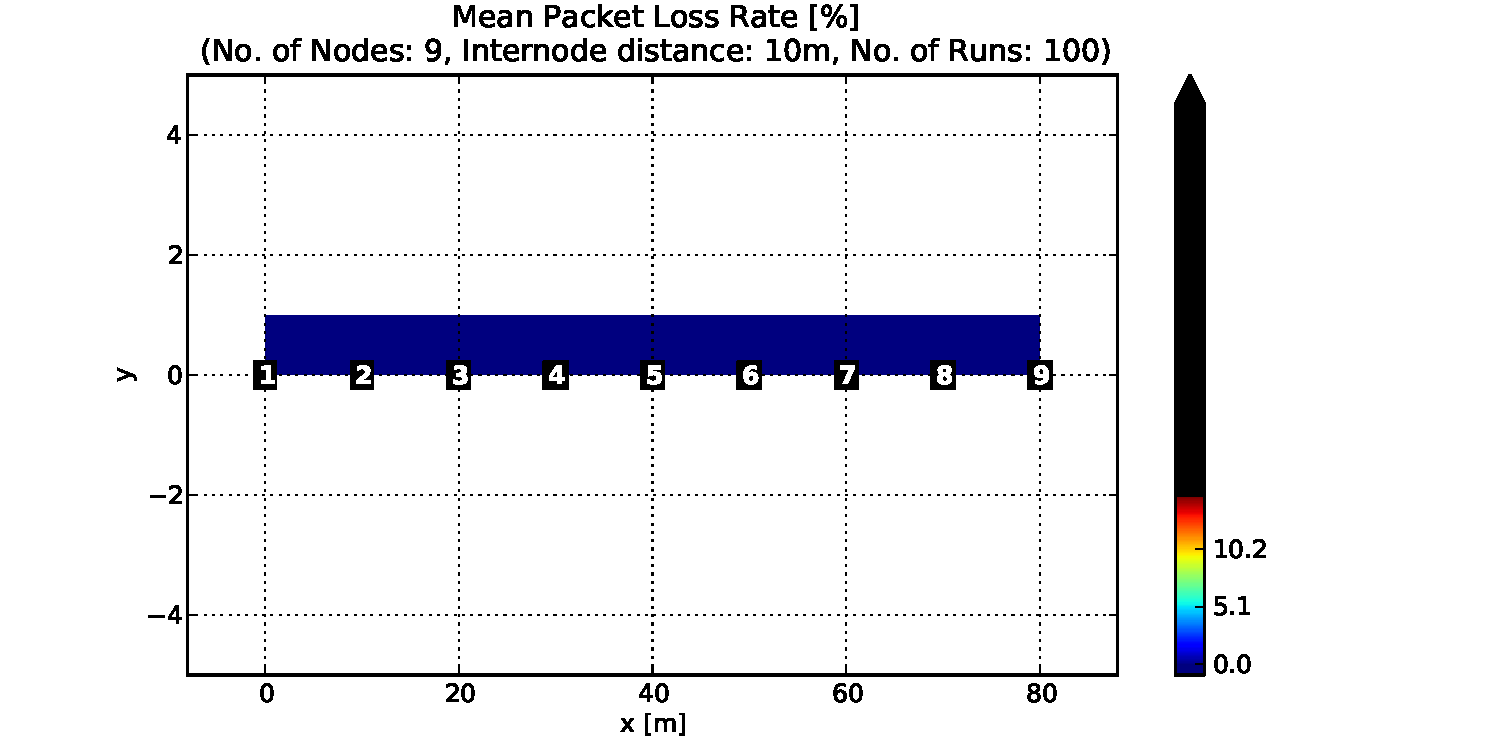
\includegraphics[trim=1.7cm 0cm 3cm 0cm, clip=true, scale=0.38]{Pics/results/9/OF0/line/dist10_montecarlo_contour_packetloss.pdf}}
    \subfloat[MRHOF]{\label{fig:9/MRHOF/line/dist10_montecarlo_contour_packetloss}
      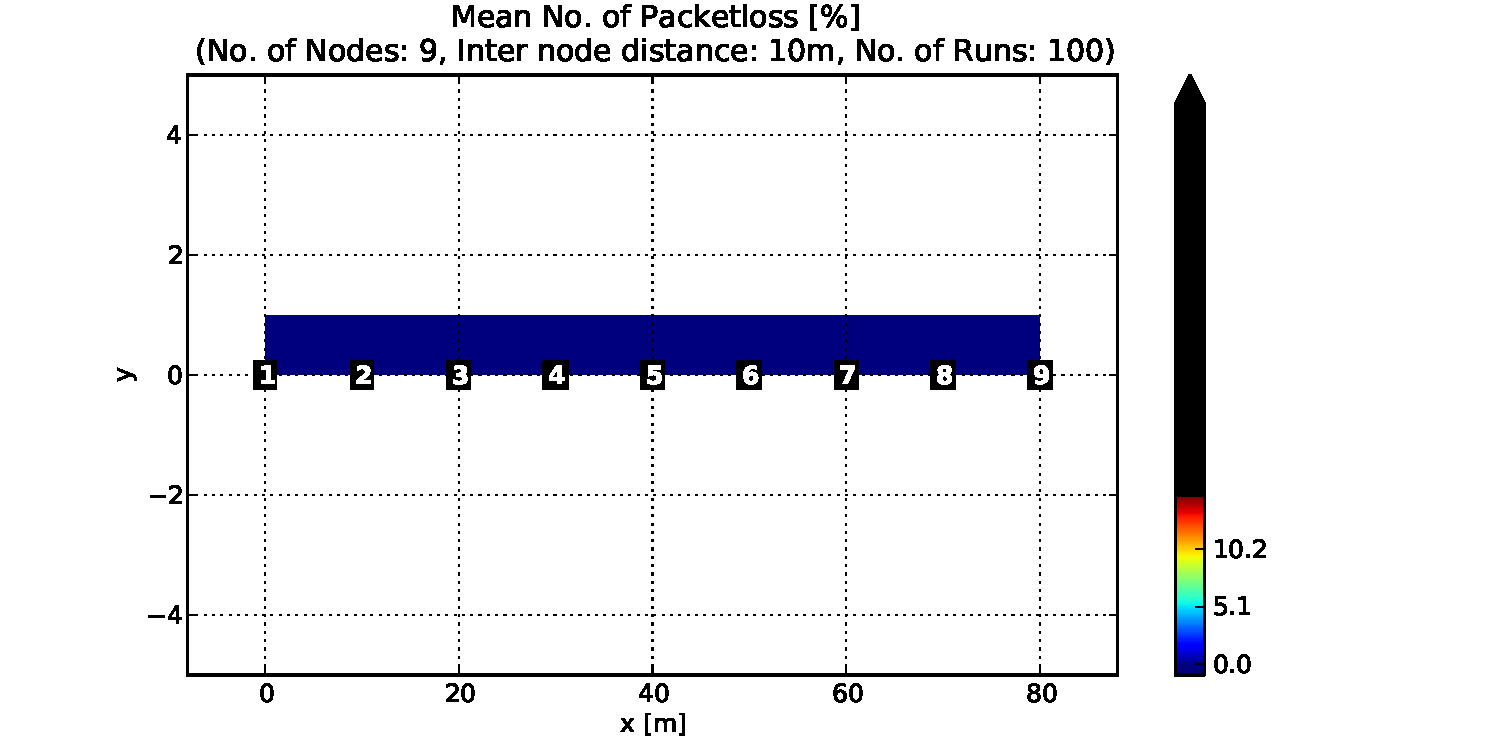
\includegraphics[trim=1.7cm 0cm 3cm 0cm, clip=true, scale=0.38]{Pics/results/9/MRHOF/line/dist10_montecarlo_contour_packetloss.pdf}}
   \caption{Mean packet loss rate: 9-node line scenario with 10~m inter-node distance}
   \label{fig:pl_9_line_10}
    \vspace{-20pt}
\end{figure}

\begin{figure}[htpb]
  \centering
    \leavevmode
    \subfloat[OF0]{\label{fig:9/OF0/line/dist50_montecarlo_contour_packetloss}
    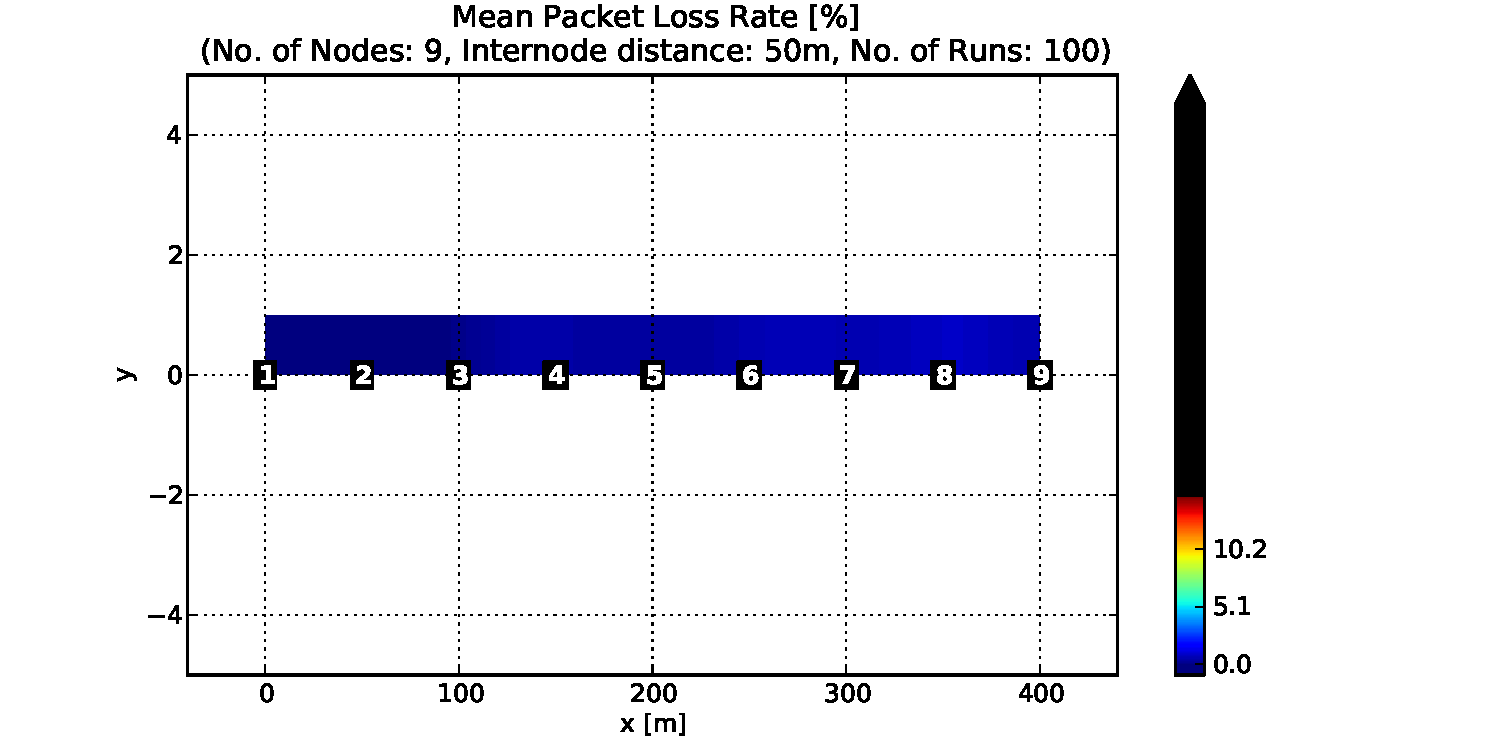
\includegraphics[trim=1.7cm 0cm 3cm 0cm, clip=true, scale=0.38]   {Pics/results/9/OF0/line/dist50_montecarlo_contour_packetloss.pdf}}
    \subfloat[MRHOF]{\label{fig:9/MRHOF/line/dist50_montecarlo_contour_packetloss}
      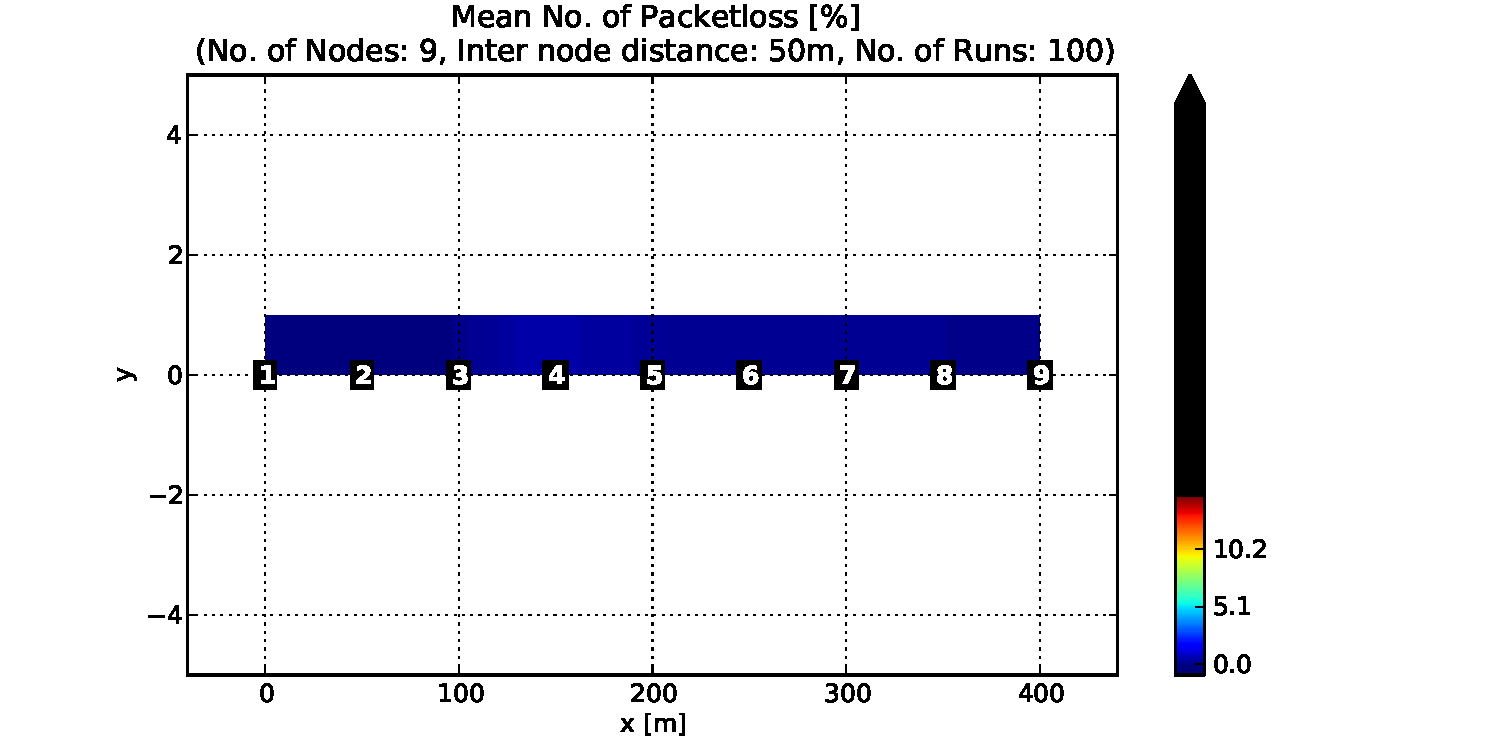
\includegraphics[trim=1.7cm 0cm 3cm 0cm, clip=true, scale=0.38]{Pics/results/9/MRHOF/line/dist50_montecarlo_contour_packetloss.pdf}}
   \caption{Mean packet loss rate: 9-node line scenario with 50~m inter-node distance}
   \label{fig:pl_9_line_50}
    \vspace{-20pt}
\end{figure}

\begin{figure}[htpb]
  \centering
    \leavevmode
    \subfloat[OF0]{\label{fig:9/OF0/line/dist100_montecarlo_contour_packetloss}
     \includegraphics[trim=1.7cm 0cm 3cm 0cm, clip=true, scale=0.38]{Pics/results/9/OF0/line/dist100_montecarlo_contour_packetloss.pdf}}
    \subfloat[MRHOF]{\label{fig:9/MRHOF/line/dist100_montecarlo_contour_packetloss}
     \includegraphics[trim=1.7cm 0cm 3cm 0cm, clip=true, scale=0.38]{Pics/results/9/MRHOF/line/dist100_montecarlo_contour_packetloss.pdf}}
  \caption{Mean packet loss rate: 9-node line scenario with 100~m inter-node distance}
  \label{fig:pl_9_line_100}
   \vspace{-20pt}
\end{figure}

%%%%%%%%%%%%%%%%%%%%%%%%%%%%%%%%%%%%%%% line 16 %%%%%%%%%%%%%%%%%%%%%%%%%%%%%%%%%%%%%%%%

\begin{figure}[p]
  \centering
    \leavevmode
    \subfloat[OF0]{\label{fig:16/OF0/line/dist10_montecarlo_contour_packetloss}
      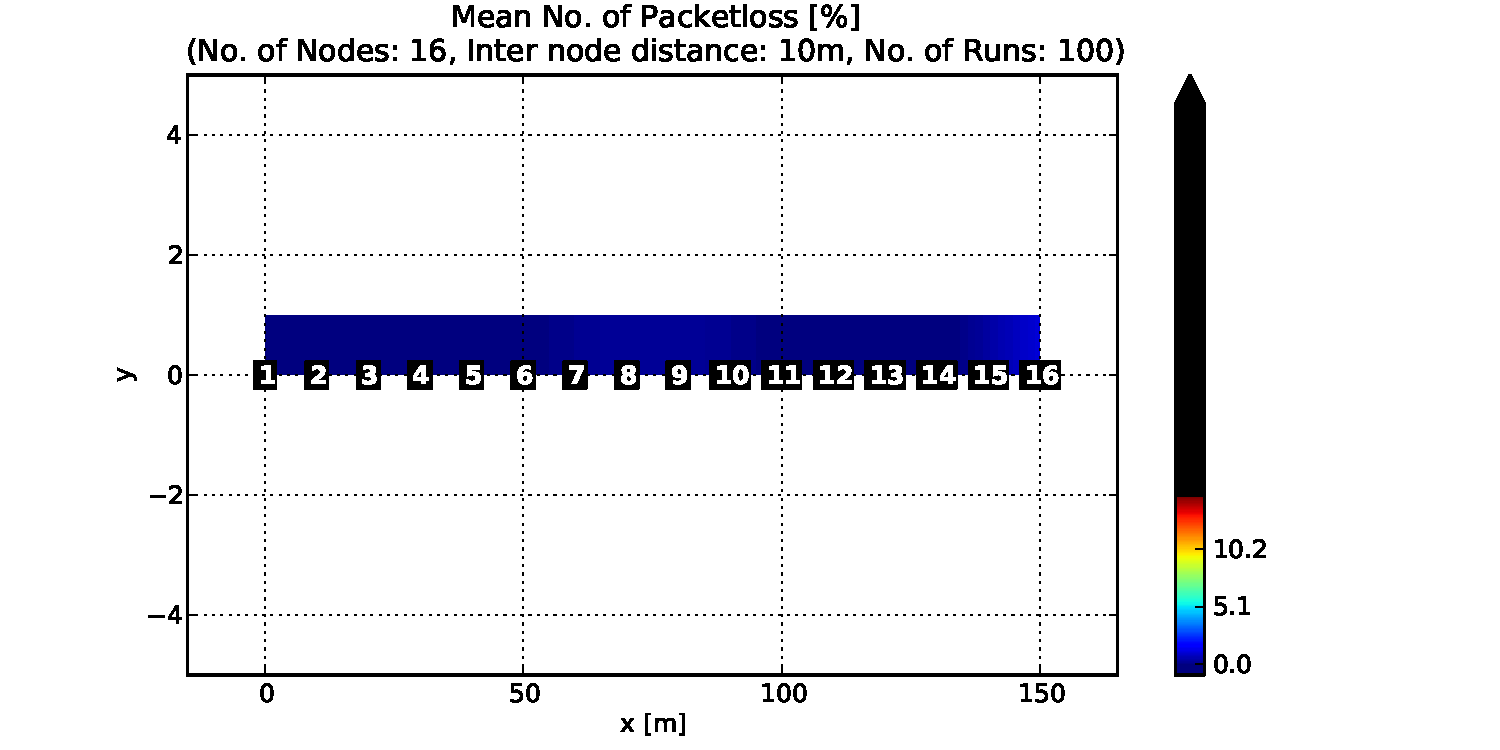
\includegraphics[trim=1.7cm 0cm 3cm 0cm, clip=true, scale=0.38]{Pics/results/16/OF0/line/dist10_montecarlo_contour_packetloss.pdf}}
    \subfloat[MRHOF]{\label{fig:16/MRHOF/line/dist10_montecarlo_contour_packetloss}
      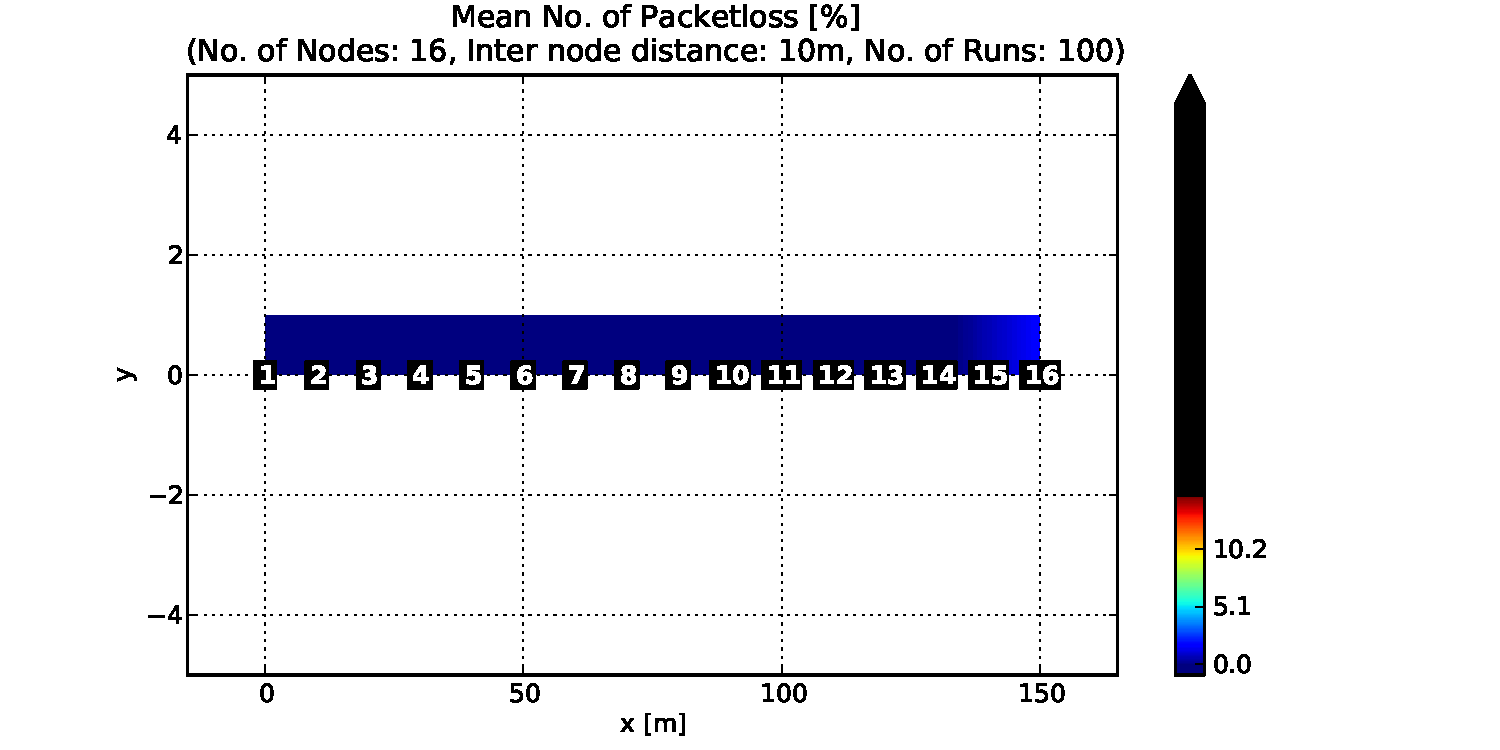
\includegraphics[trim=1.7cm 0cm 3cm 0cm, clip=true, scale=0.38]{Pics/results/16/MRHOF/line/dist10_montecarlo_contour_packetloss.pdf}}
   \caption{Mean packet loss rate: 16-node line scenario with 10~m inter-node distance}
   \label{fig:pl_16_line_10}
    \vspace{-20pt}
\end{figure}

\begin{figure}[p]
  \centering
    \leavevmode
    \subfloat[OF0]{\label{fig:16/OF0/line/dist50_montecarlo_contour_packetloss}
    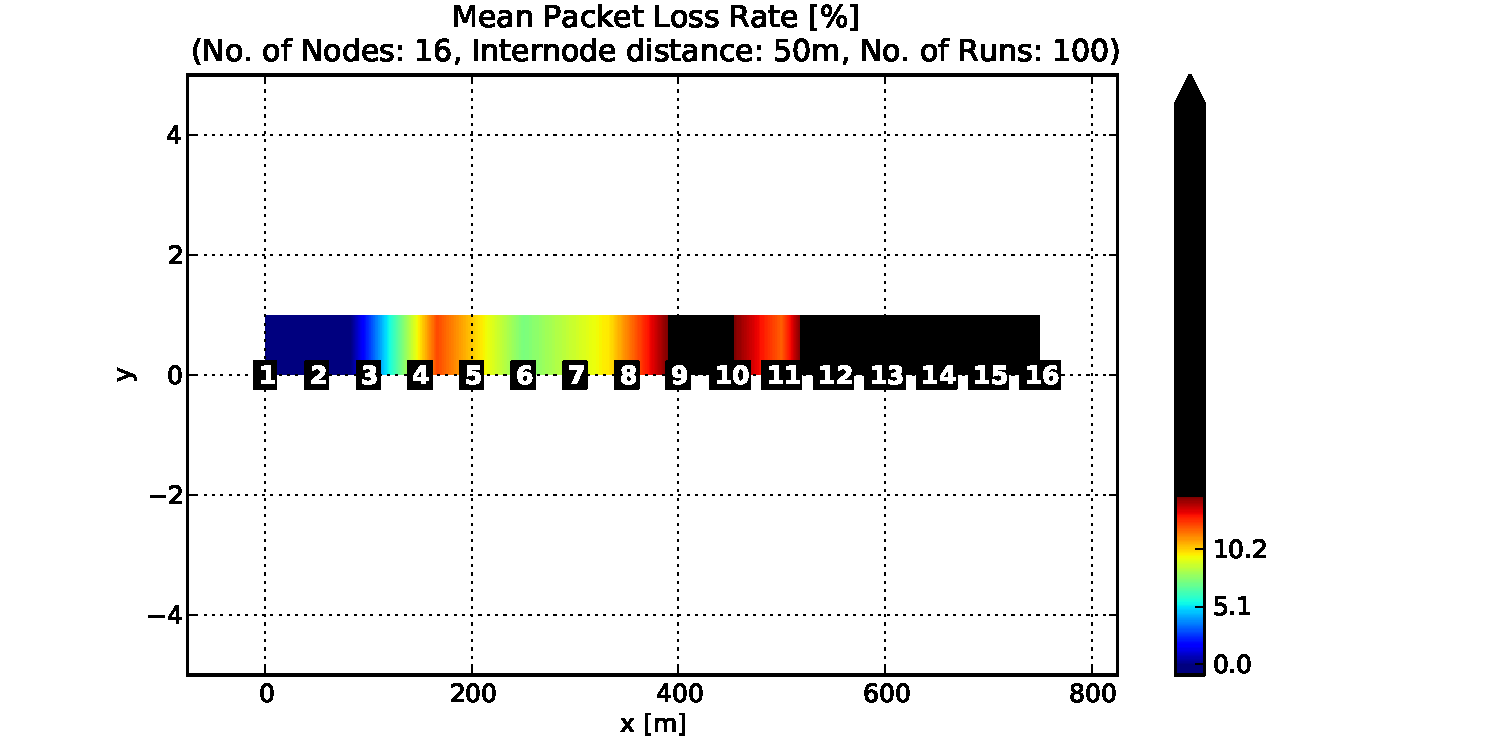
\includegraphics[trim=1.7cm 0cm 3cm 0cm, clip=true, scale=0.38]   {Pics/results/16/OF0/line/dist50_montecarlo_contour_packetloss.pdf}}
    \subfloat[MRHOF]{\label{fig:16/MRHOF/line/dist50_montecarlo_contour_packetloss}
      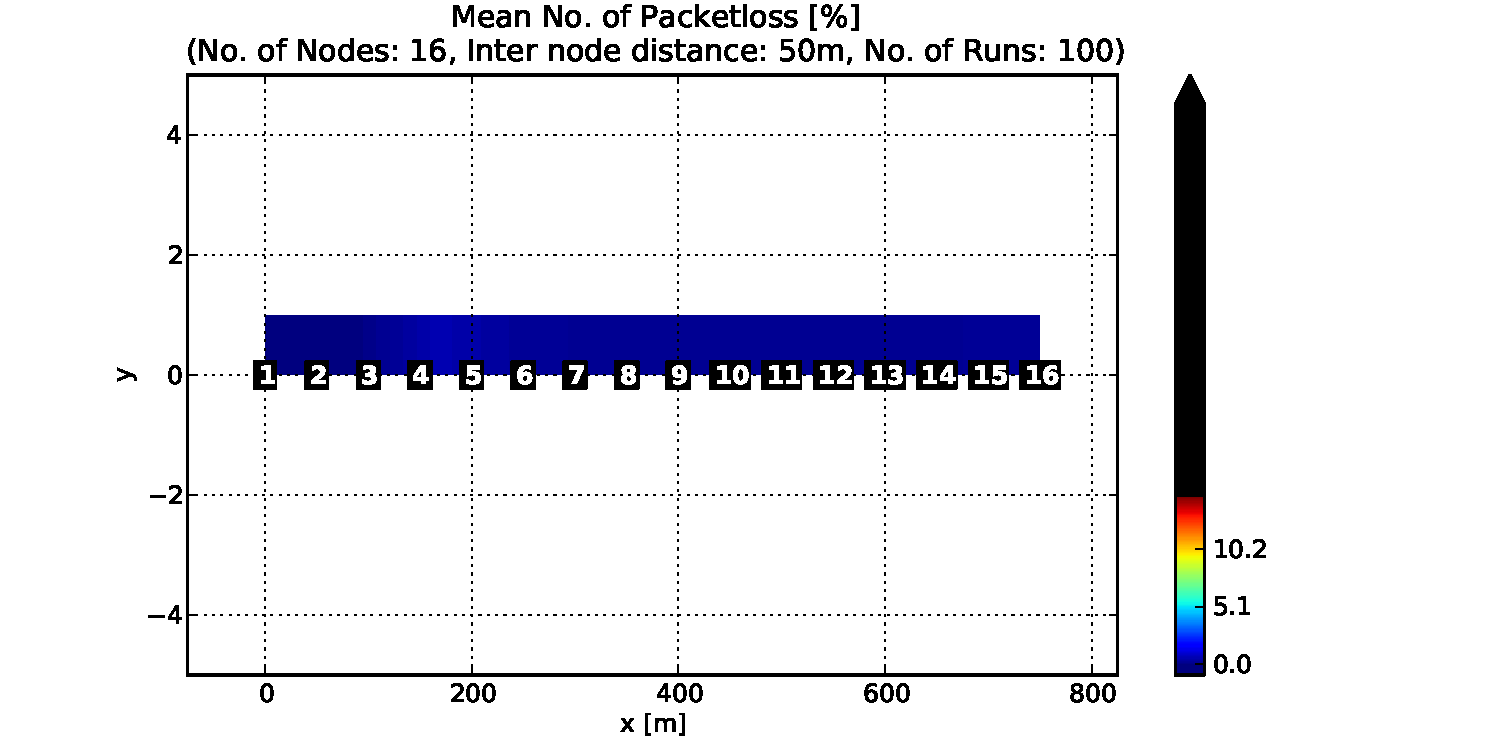
\includegraphics[trim=1.7cm 0cm 3cm 0cm, clip=true, scale=0.38]{Pics/results/16/MRHOF/line/dist50_montecarlo_contour_packetloss.pdf}}
   \caption{Mean packet loss rate: 16-node line scenario with 50~m inter-node distance}
   \label{fig:pl_16_line_50}
    \vspace{-20pt}
\end{figure}

\begin{figure}[p]
  \centering
    \leavevmode
    \subfloat[OF0]{\label{fig:16/OF0/line/dist100_montecarlo_contour_packetloss}
     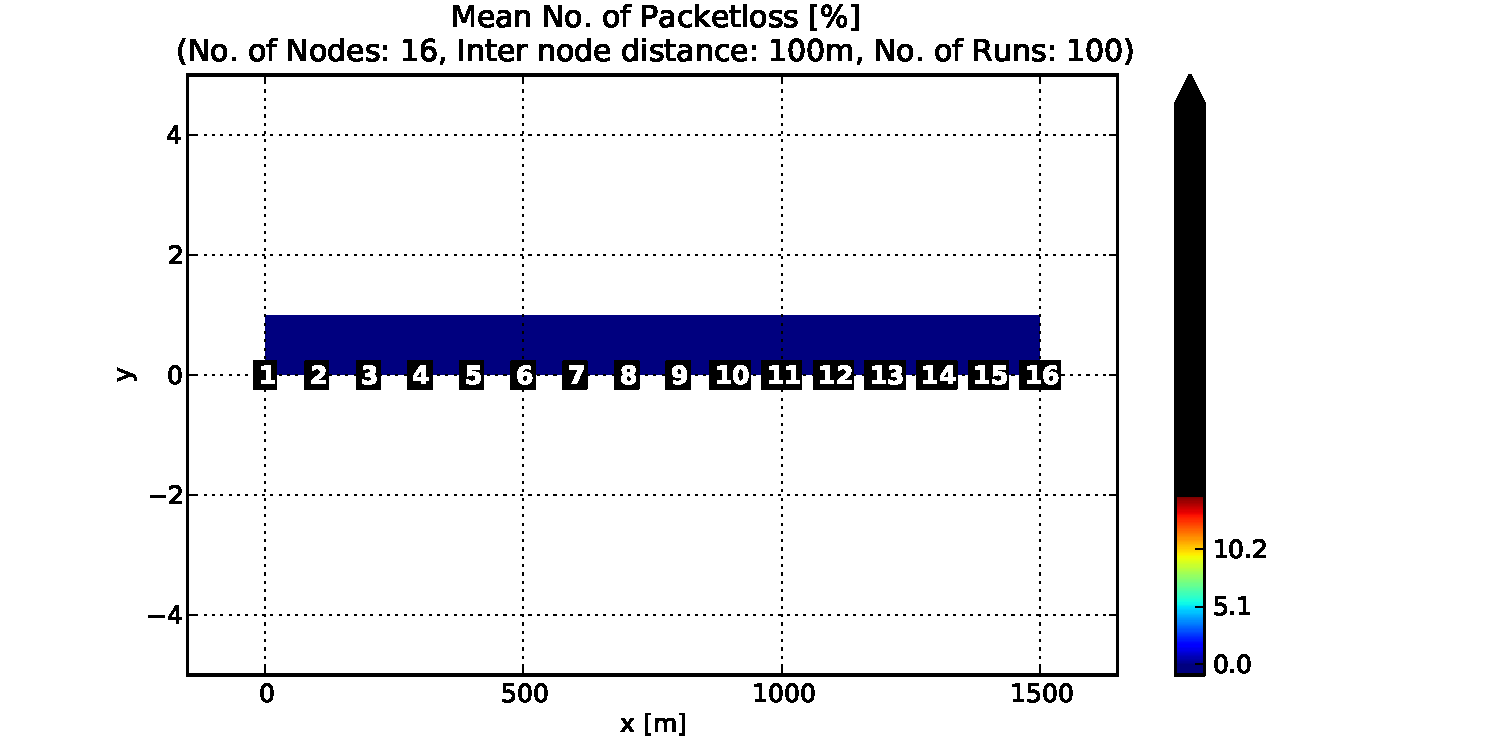
\includegraphics[trim=1.7cm 0cm 3cm 0cm, clip=true, scale=0.38]{Pics/results/16/OF0/line/dist100_montecarlo_contour_packetloss.pdf}}
    \subfloat[MRHOF]{\label{fig:16/MRHOF/line/dist100_montecarlo_contour_packetloss}
     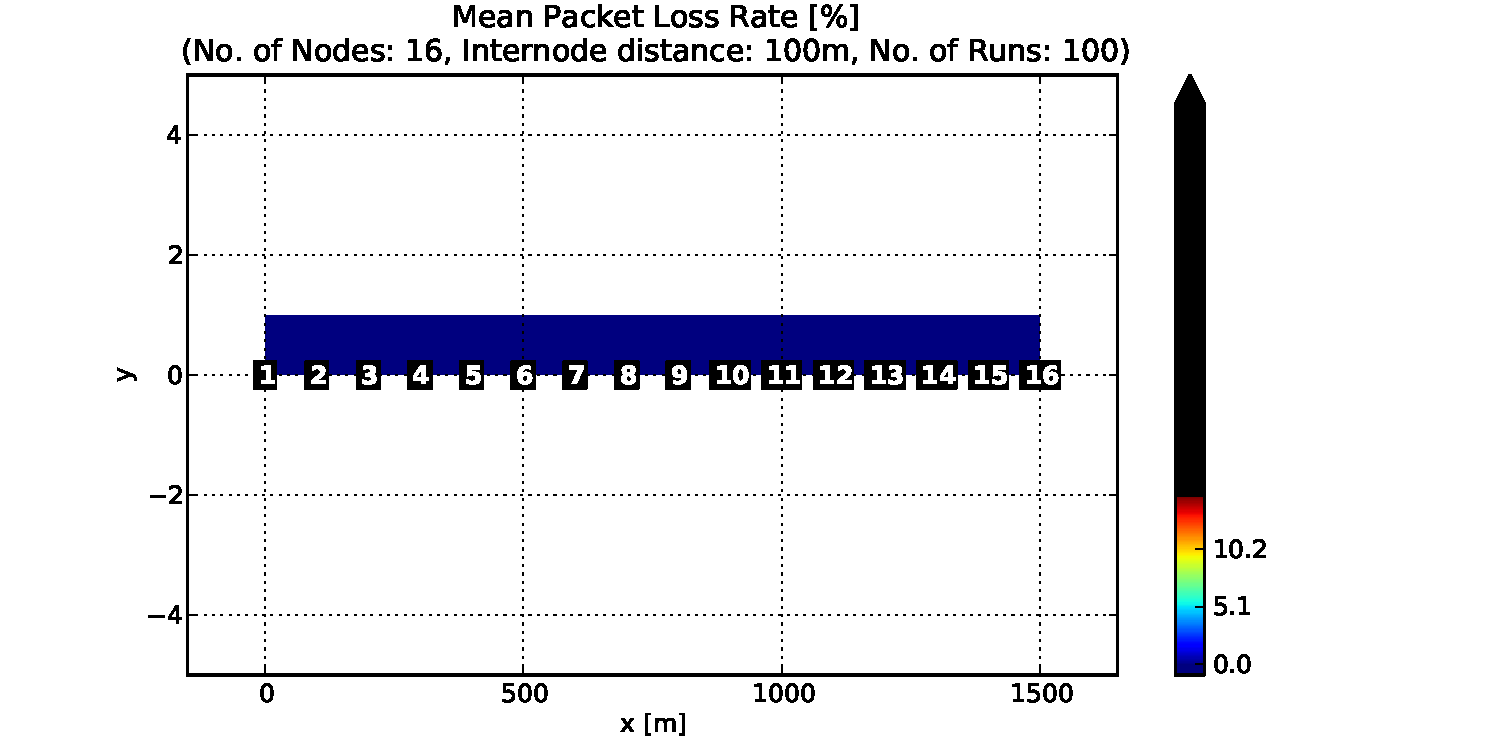
\includegraphics[trim=1.7cm 0cm 3cm 0cm, clip=true, scale=0.38]{Pics/results/16/MRHOF/line/dist100_montecarlo_contour_packetloss.pdf}}
  \caption{Mean packet loss rate: 16-node line scenario with 100~m inter-node distance}
  \label{fig:pl_16_line_100}
   \vspace{-20pt}
\end{figure}

\clearpage
\subsection{Grid Scenario}
\label{pl:grid}
The mean packet loss rate results for the grid scenario are shown in Figure~\ref{fig:pl_4_grid_10} to Figure~\ref{fig:pl_16_grid_100}.

Compared to the line scenario, the grid scenario is more complicated in terms of routing due to its higher node density and increased route options.  Under this scenario, one can see that the packet loss rate goes up with the increase of the inter-node distance due to the PRR being reduced. This phenomenon appears more obvious on the results with OF0 than those with MRHOF, showing that with OF0 the dropping of PRR gives more packet loss on OF0 than MRHOF. Furthermore, OF0 shows a high packet loss in the 16-node scenario with 50 meters inter-node distance (Figure~\ref{fig:16/OF0/grid/dist50_montecarlo_contour_packetloss}) while MRHOF gives no more than 5\% packet loss.

The packet loss rate comparison between MRHOF and OF0 shows that with OF0 a node is very likely to choose a routing parent with an unreliable link, such as a link with a low PRR; on the other hand, MRHOF with link ETX is apt to choose a link with the least estimated transmission count, therefore the parent choosing mechanism is more stable and reliable.

%%%%%%%%%%%%%%%%%%%%%%%%%%%%%%%%%%%%%%% grid 4 %%%%%%%%%%%%%%%%%%%%%%%%%%%%%%%%%%%%%%%%
\begin{figure}[p]
  \centering
   \vspace{-20pt}
    \leavevmode
    \subfloat[OF0]{\label{fig:4/OF0/grid/dist10_montecarlo_contour_packetloss}
      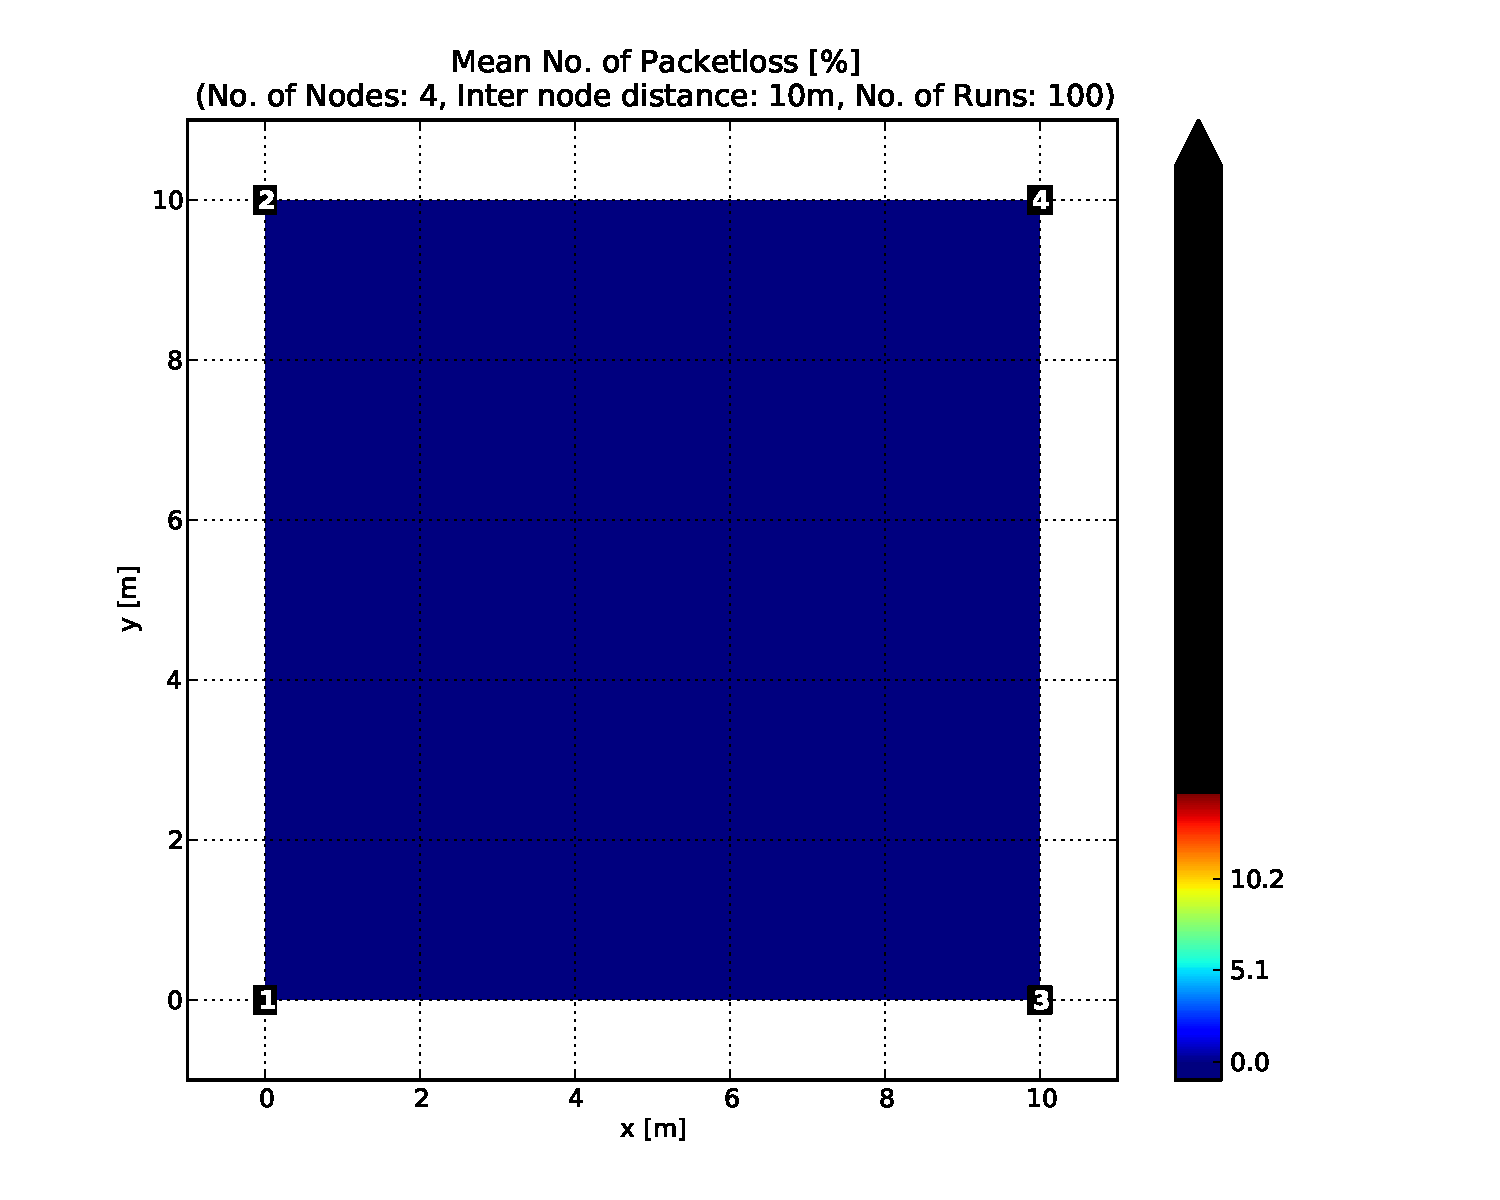
\includegraphics[trim=1.7cm 0cm 3cm 0cm, clip=true, scale=0.3]{Pics/results/4/OF0/grid/dist10_montecarlo_contour_packetloss.pdf}}
      \hspace{15pt}
    \subfloat[MRHOF]{\label{fig:4/MRHOF/grid/dist10_montecarlo_contour_packetloss}
      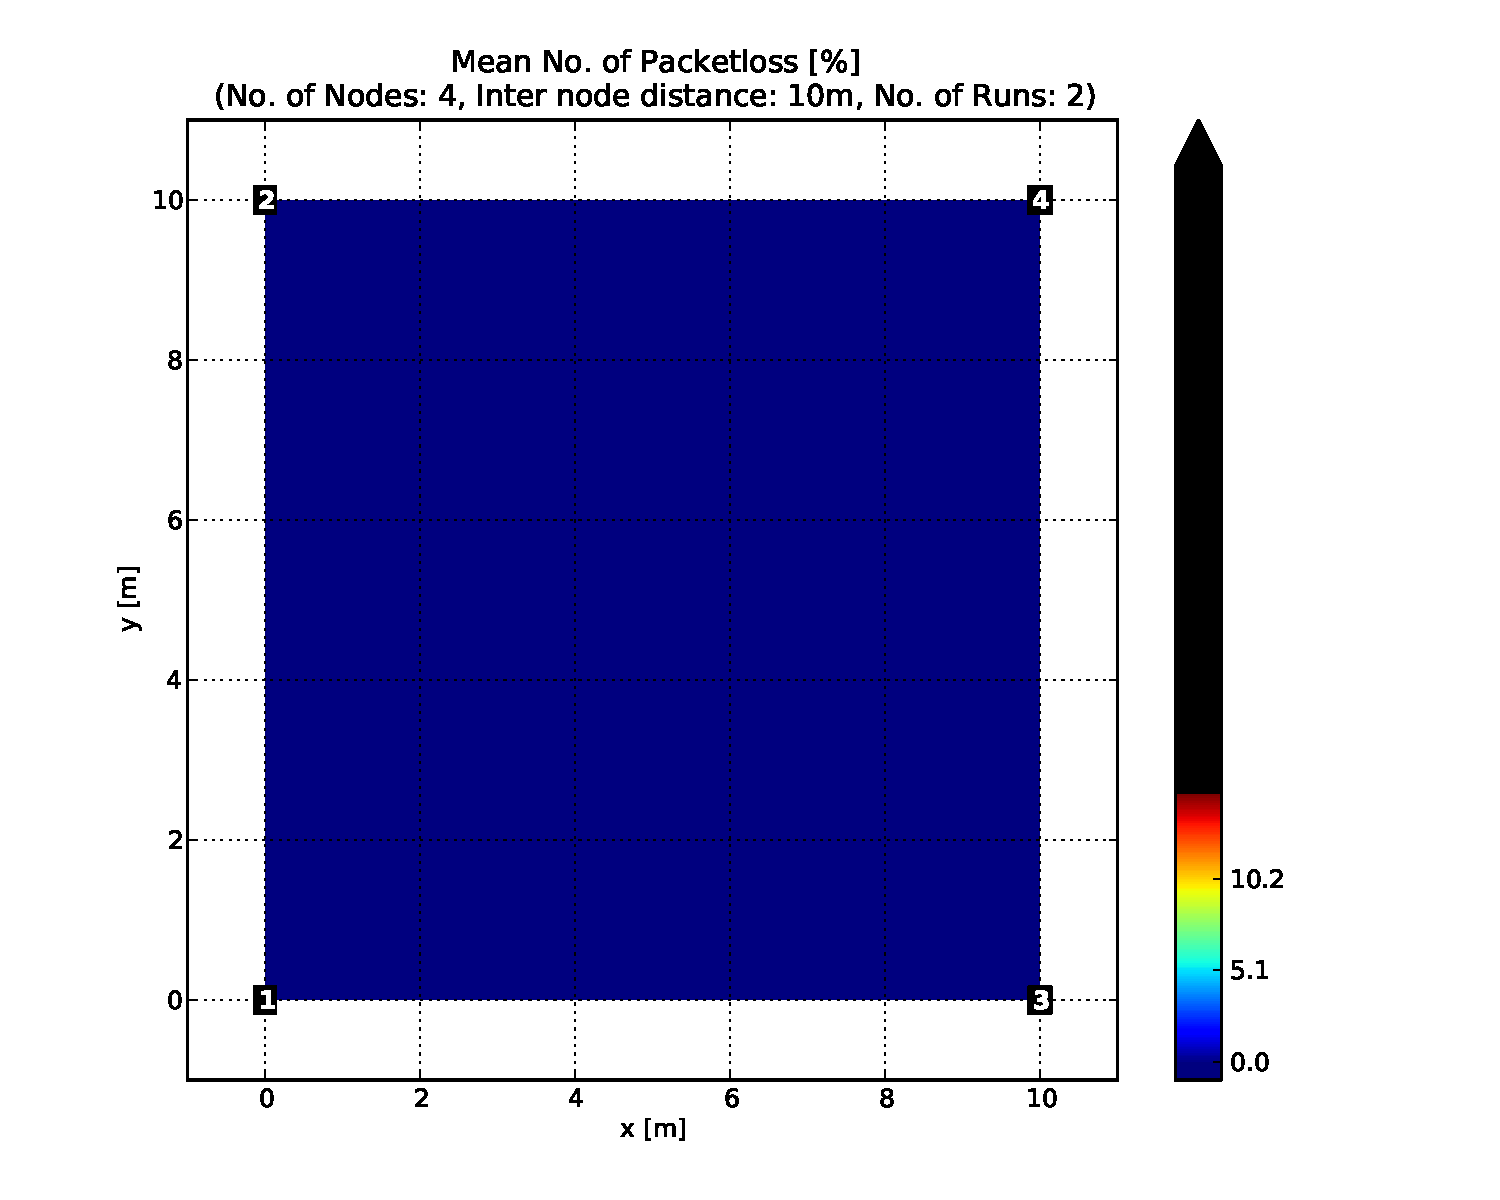
\includegraphics[trim=1.7cm 0cm 3cm 0cm, clip=true, scale=0.3]{Pics/results/4/MRHOF/grid/dist10_montecarlo_contour_packetloss.pdf}}
   \caption{Mean packet loss rate: 4-node grid scenario with 10~m inter-node distance}
   \label{fig:pl_4_grid_10}
    \vspace{-25pt}
\end{figure}

\begin{figure}[p]
  \centering
    \leavevmode
    \subfloat[OF0]{\label{fig:4/OF0/grid/dist50_montecarlo_contour_packetloss}
    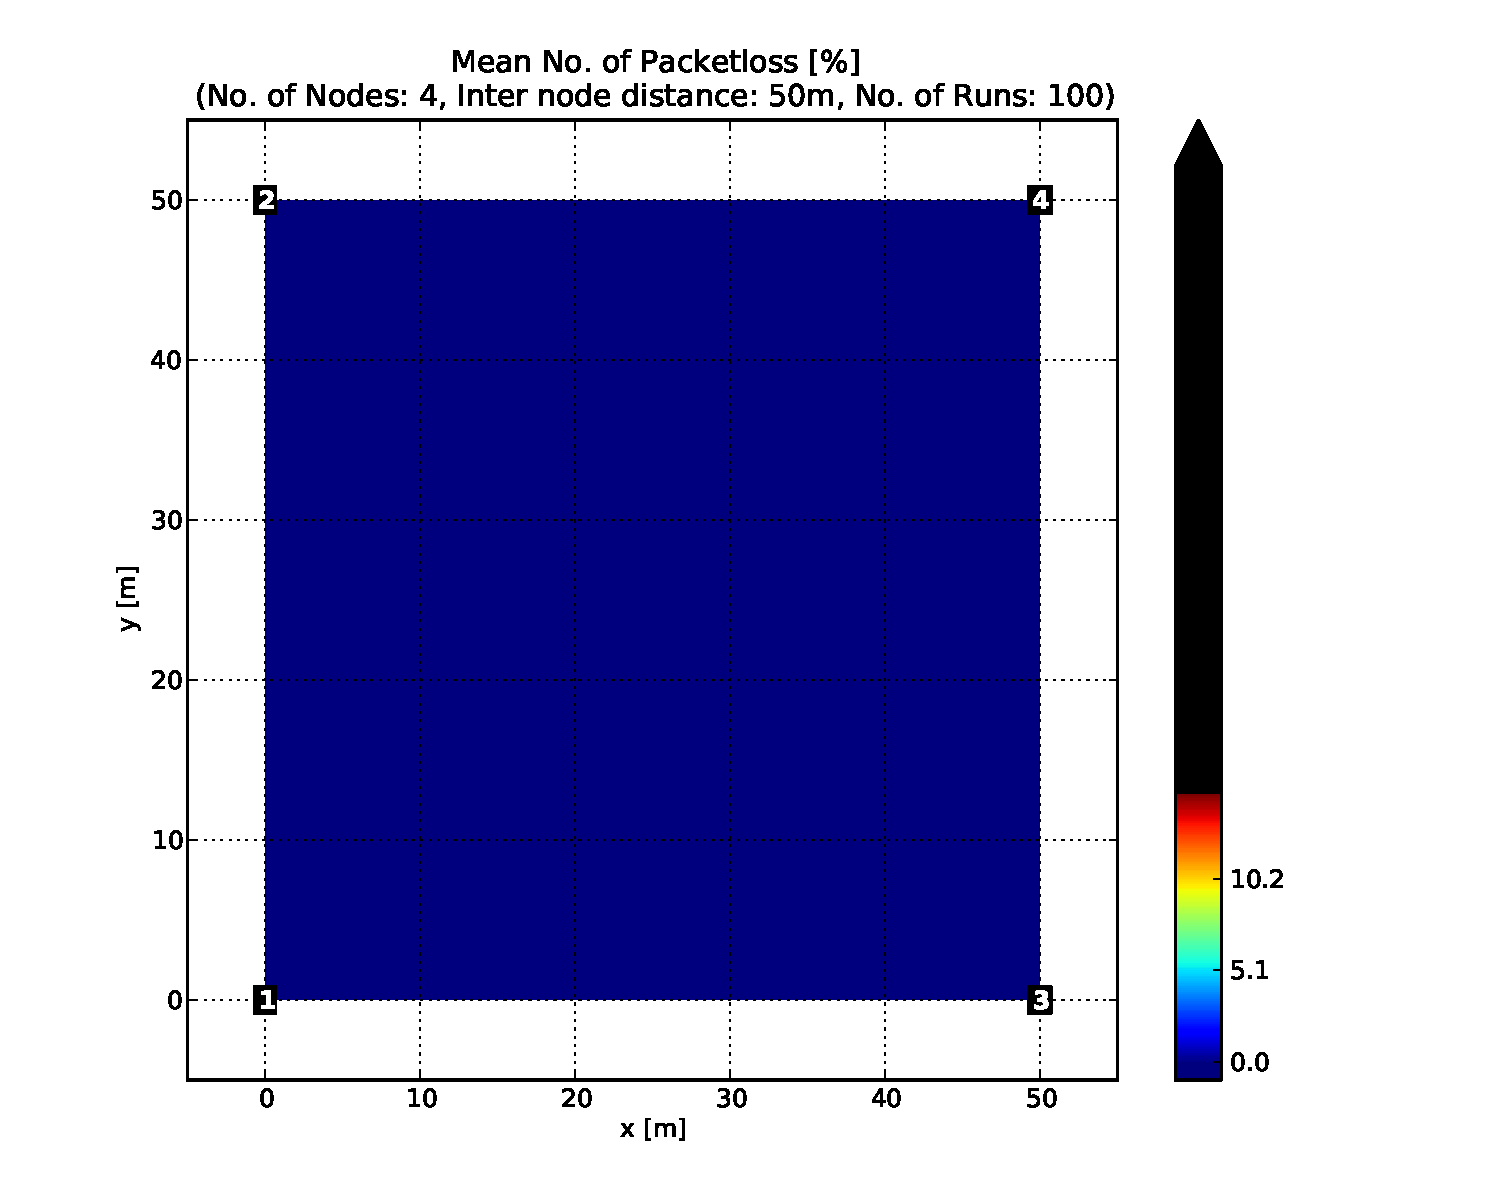
\includegraphics[trim=1.7cm 0cm 3cm 0cm, clip=true, scale=0.3]   {Pics/results/4/OF0/grid/dist50_montecarlo_contour_packetloss.pdf}}
    \hspace{15pt}
    \subfloat[MRHOF]{\label{fig:4/MRHOF/grid/dist50_montecarlo_contour_packetloss}
      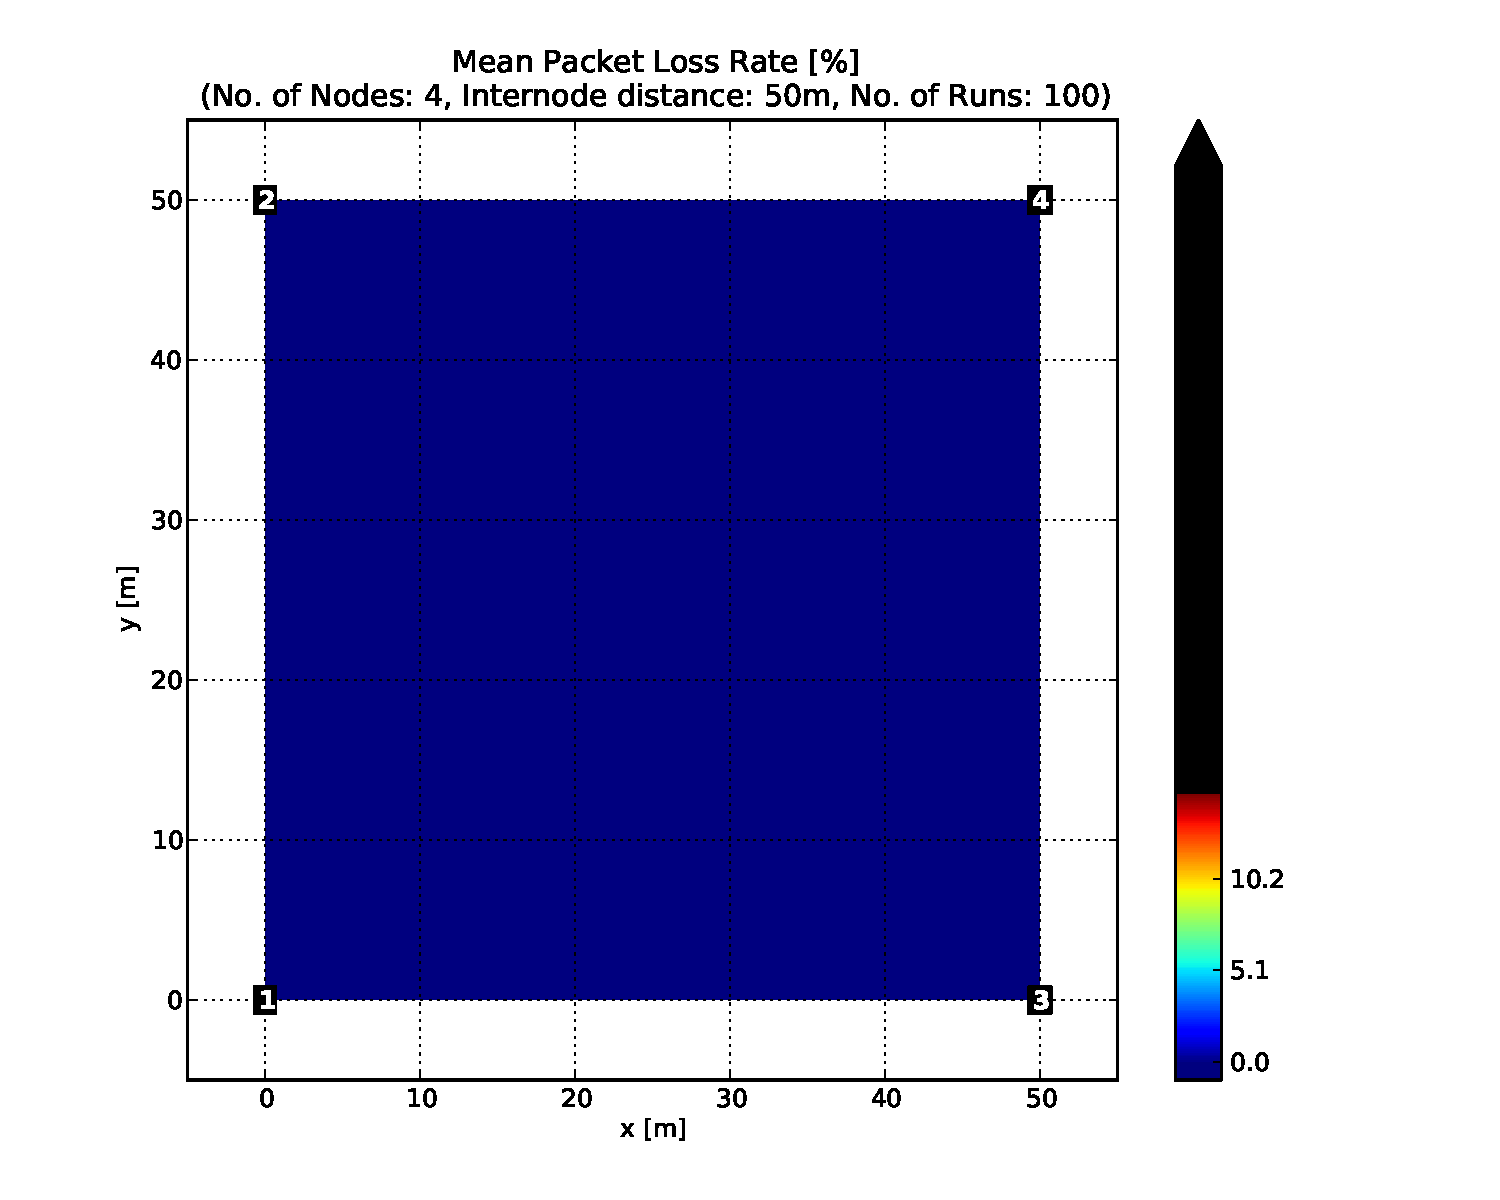
\includegraphics[trim=1.7cm 0cm 3cm 0cm, clip=true, scale=0.3]{Pics/results/4/MRHOF/grid/dist50_montecarlo_contour_packetloss.pdf}}
   \caption{Mean packet loss rate: 4-node grid scenario with 50~m inter-node distance}
   \label{fig:pl_4_grid_50}
    \vspace{-25pt}
\end{figure}

\begin{figure}[p]
  \centering
    \leavevmode
    \subfloat[OF0]{\label{fig:4/OF0/grid/dist100_montecarlo_contour_packetloss}
     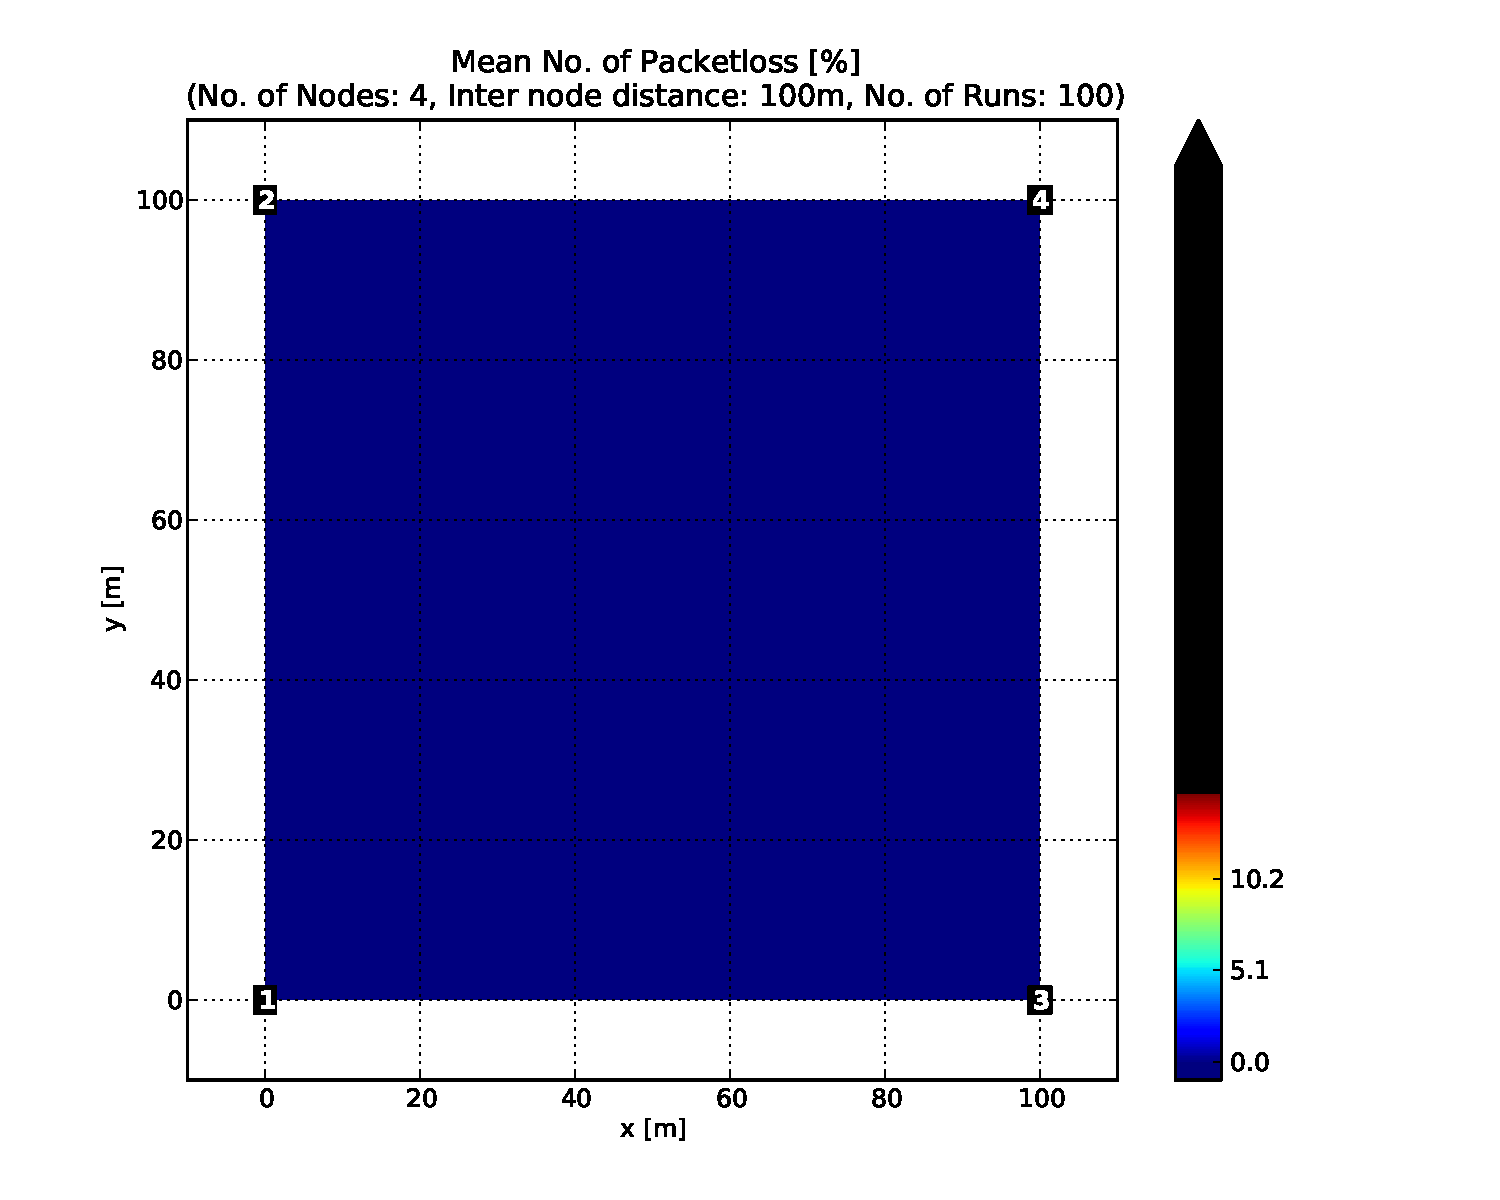
\includegraphics[trim=1.7cm 0cm 3cm 0cm, clip=true, scale=0.3]{Pics/results/4/OF0/grid/dist100_montecarlo_contour_packetloss.pdf}}
     \hspace{15pt}
    \subfloat[MRHOF]{\label{fig:4/MRHOF/grid/dist100_montecarlo_contour_packetloss}
     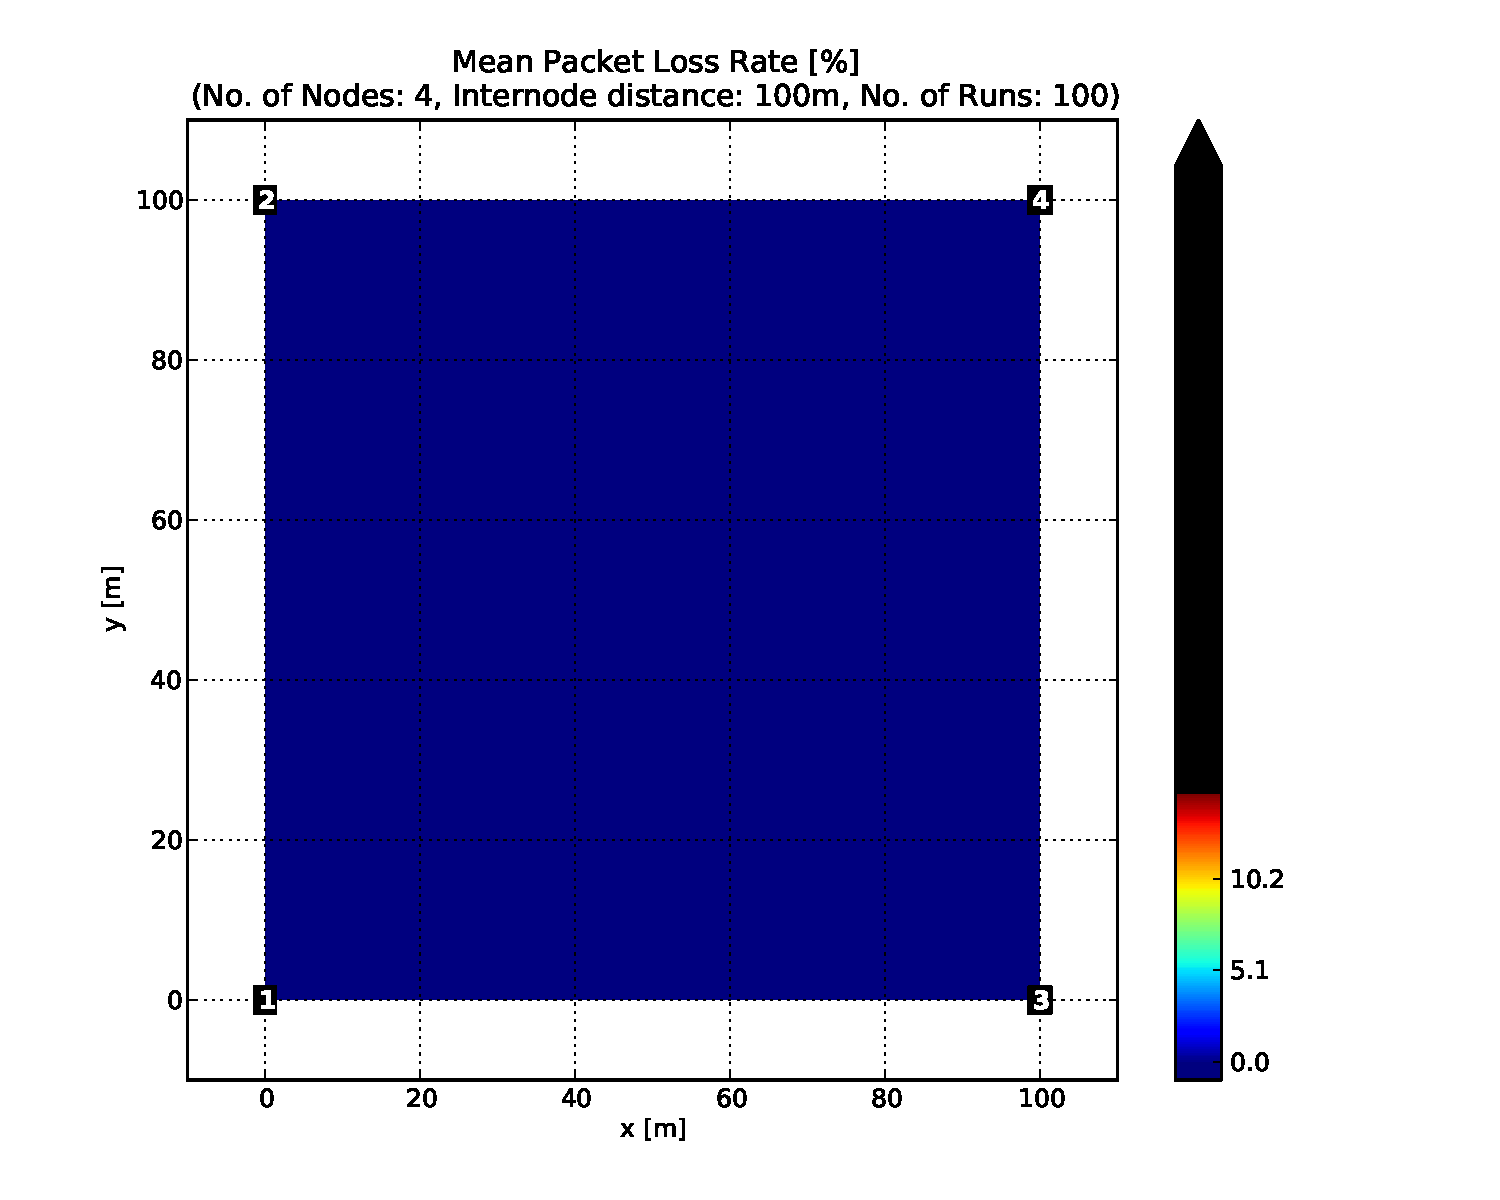
\includegraphics[trim=1.7cm 0cm 3cm 0cm, clip=true, scale=0.3]{Pics/results/4/MRHOF/grid/dist100_montecarlo_contour_packetloss.pdf}}
  \caption{Mean packet loss rate: 4-node grid scenario with 100~m inter-node distance}
  \label{fig:pl_4_grid_100}
   \vspace{-25pt}
\end{figure}

%%%%%%%%%%%%%%%%%%%%%%%%%%%%%%%%%%%%%%% grid 9 %%%%%%%%%%%%%%%%%%%%%%%%%%%%%%%%%%%%%%%%

\begin{figure}[p]
  \centering
   \vspace{-20pt}
    \leavevmode
    \subfloat[OF0]{\label{fig:9/OF0/grid/dist10_montecarlo_contour_packetloss}
      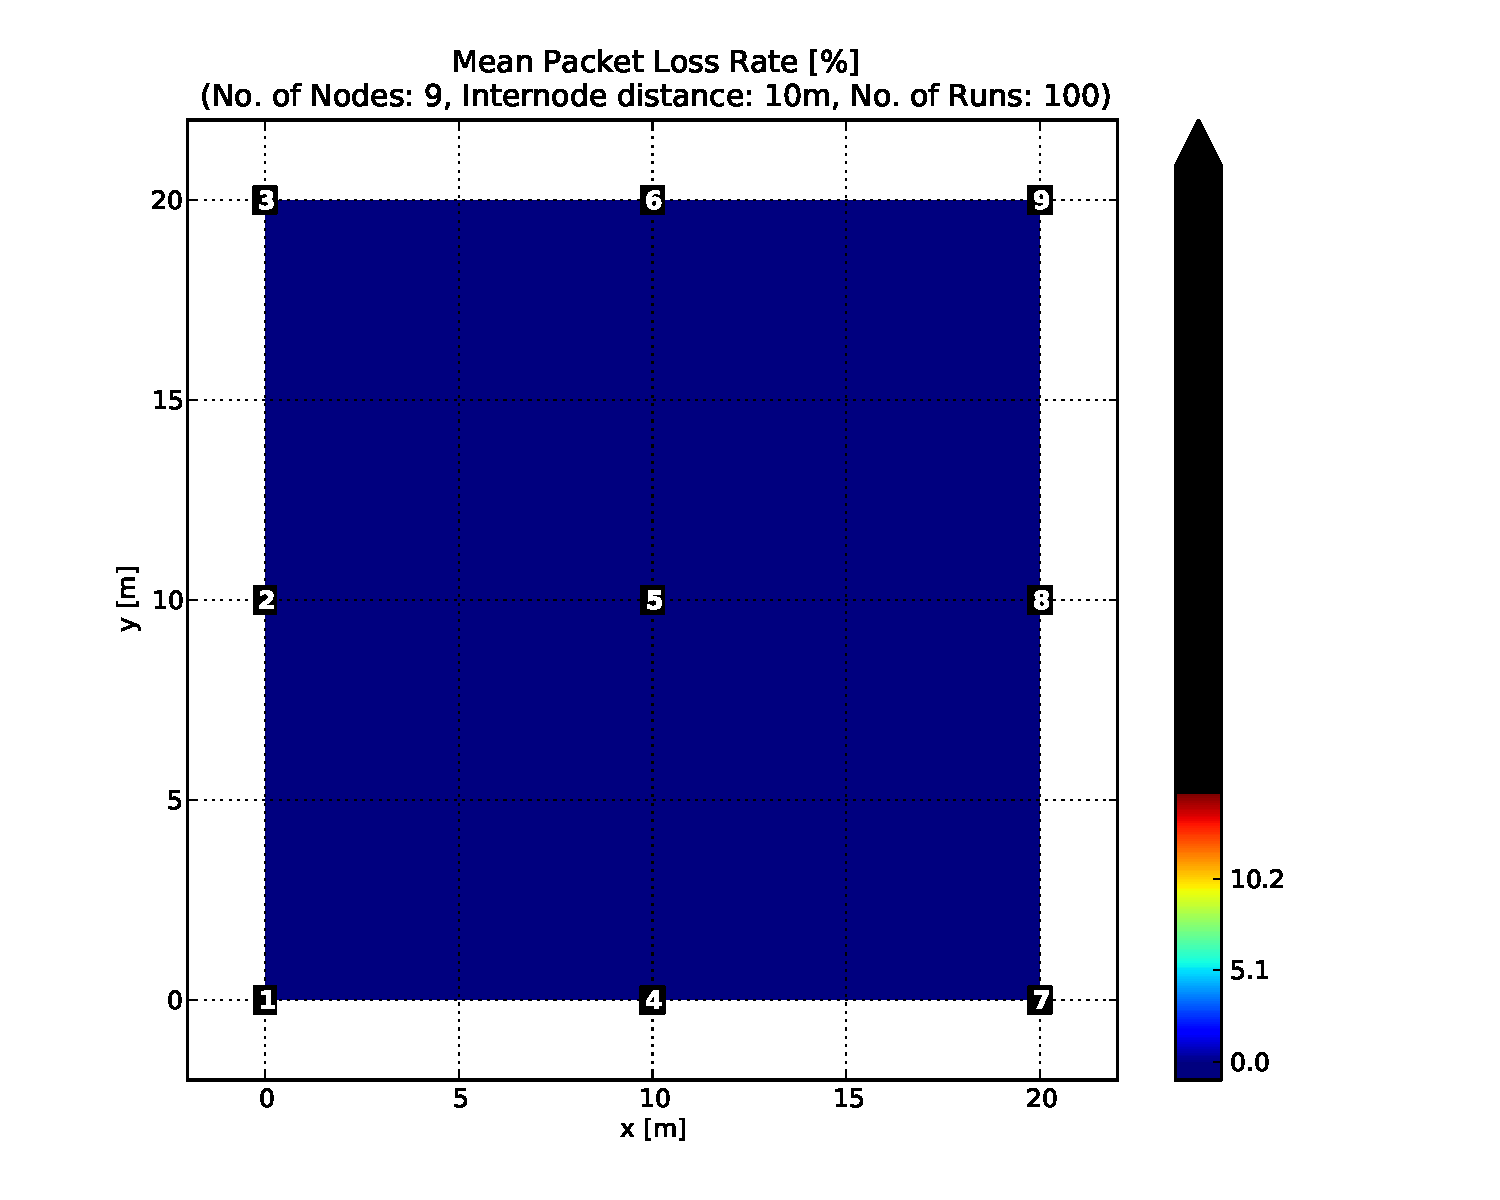
\includegraphics[trim=1.7cm 0cm 3cm 0cm, clip=true, scale=0.3]{Pics/results/9/OF0/grid/dist10_montecarlo_contour_packetloss.pdf}}
      \hspace{15pt}
    \subfloat[MRHOF]{\label{fig:9/MRHOF/grid/dist10_montecarlo_contour_packetloss}
      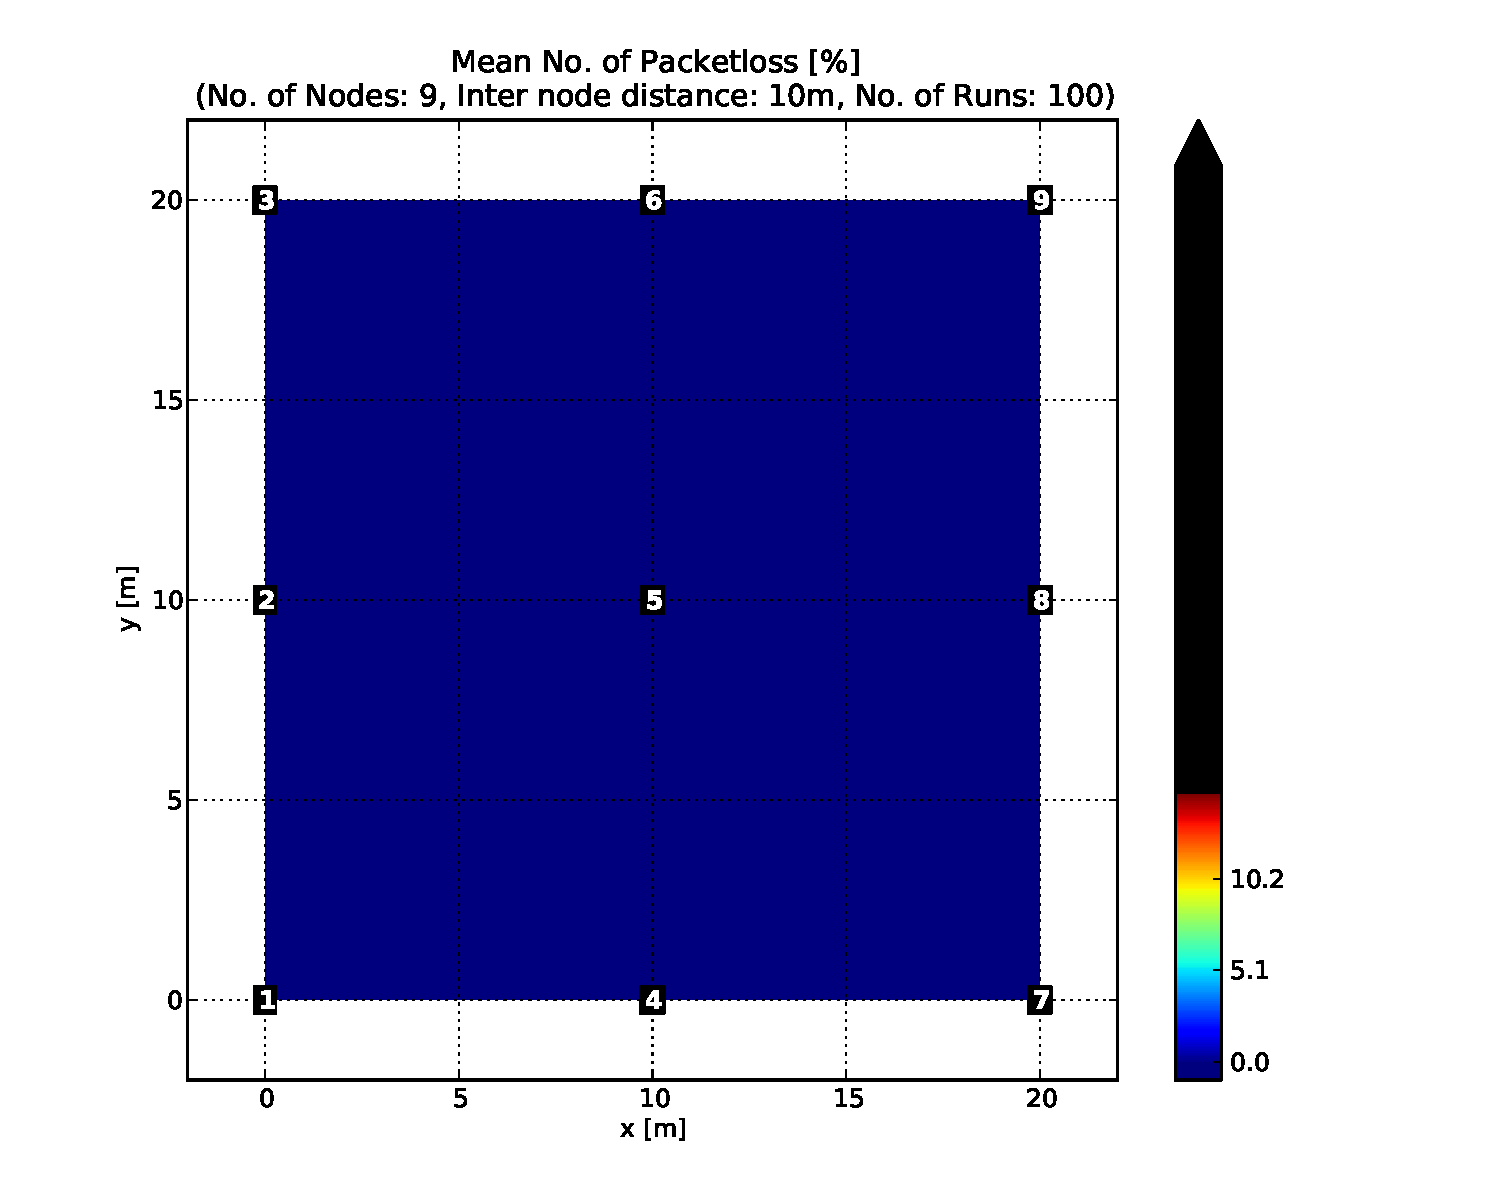
\includegraphics[trim=1.7cm 0cm 3cm 0cm, clip=true, scale=0.3]{Pics/results/9/MRHOF/grid/dist10_montecarlo_contour_packetloss.pdf}}
   \caption{Mean packet loss rate: 9-node grid scenario with 10~m inter-node distance}
   \label{fig:pl_9_grid_10}
    \vspace{-25pt}
\end{figure}

\begin{figure}[p]
  \centering
    \leavevmode
    \subfloat[OF0]{\label{fig:9/OF0/grid/dist50_montecarlo_contour_packetloss}
    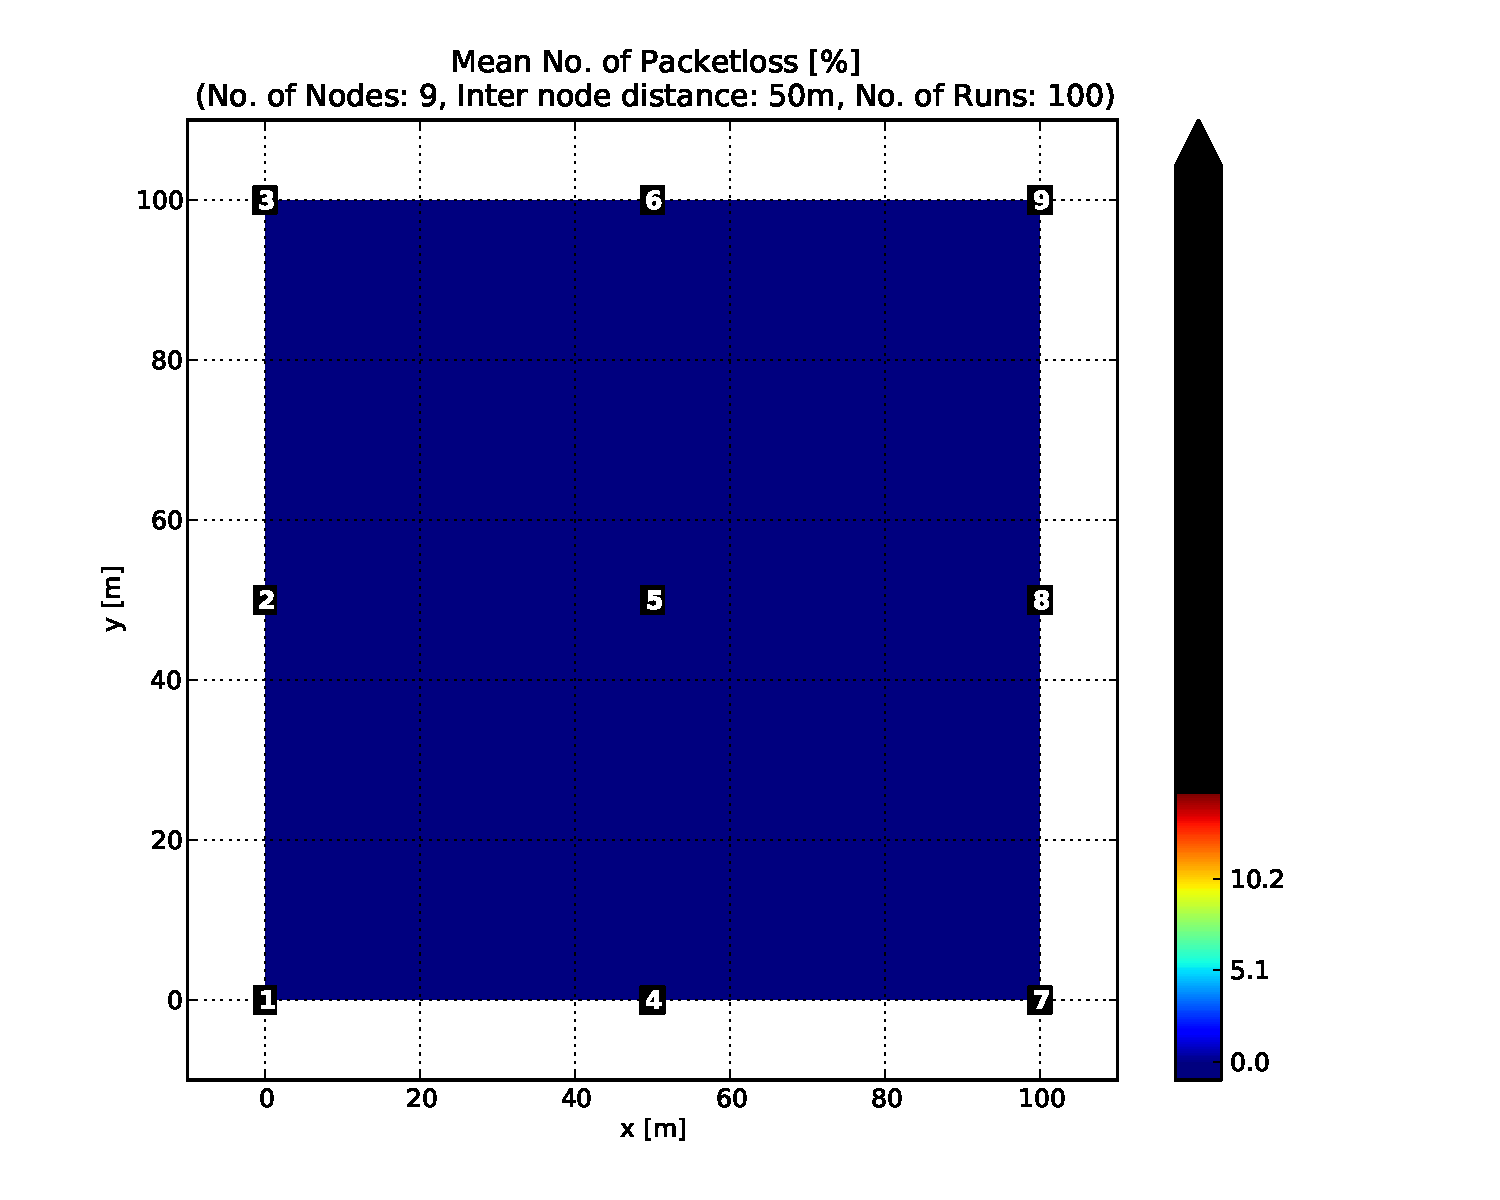
\includegraphics[trim=1.7cm 0cm 3cm 0cm, clip=true, scale=0.3]   {Pics/results/9/OF0/grid/dist50_montecarlo_contour_packetloss.pdf}}
    \hspace{15pt}
    \subfloat[MRHOF]{\label{fig:9/MRHOF/grid/dist50_montecarlo_contour_packetloss}
      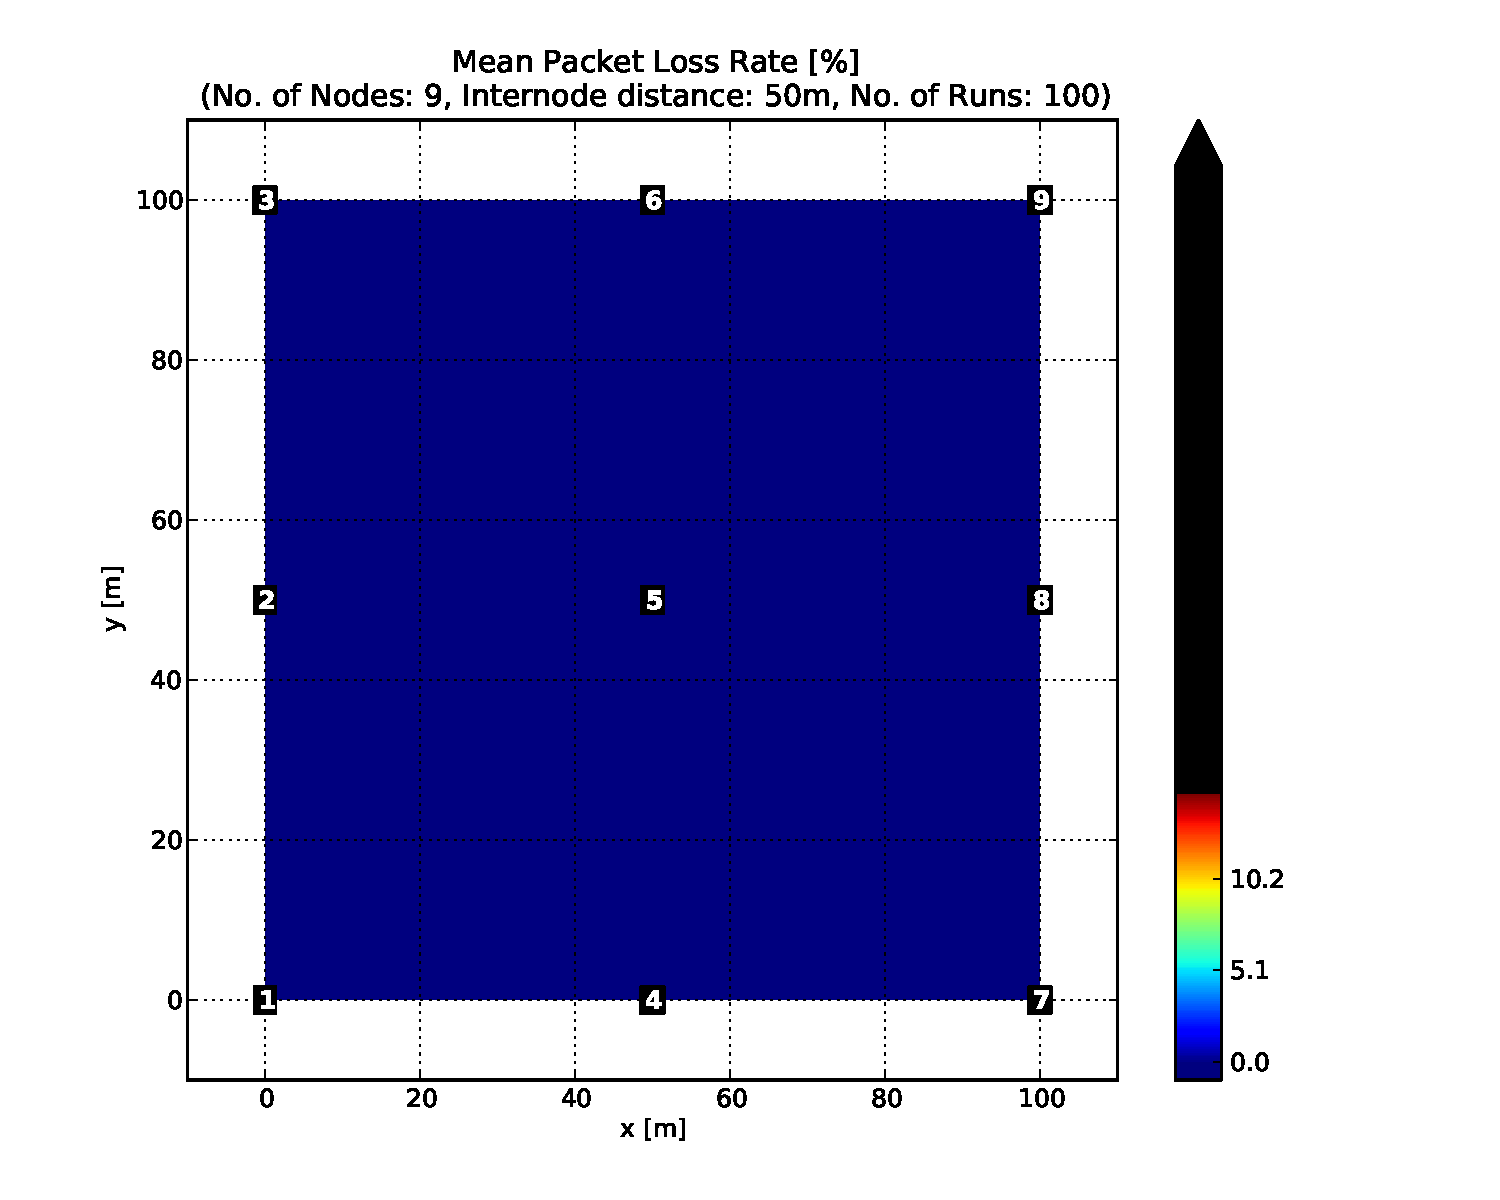
\includegraphics[trim=1.7cm 0cm 3cm 0cm, clip=true, scale=0.3]{Pics/results/9/MRHOF/grid/dist50_montecarlo_contour_packetloss.pdf}}
   \caption{Mean packet loss rate: 9-node grid scenario with 50~m inter-node distance}
   \label{fig:pl_9_grid_50}
    \vspace{-25pt}
\end{figure}

\begin{figure}[p]
  \centering
    \leavevmode
    \subfloat[OF0]{\label{fig:9/OF0/grid/dist100_montecarlo_contour_packetloss}
     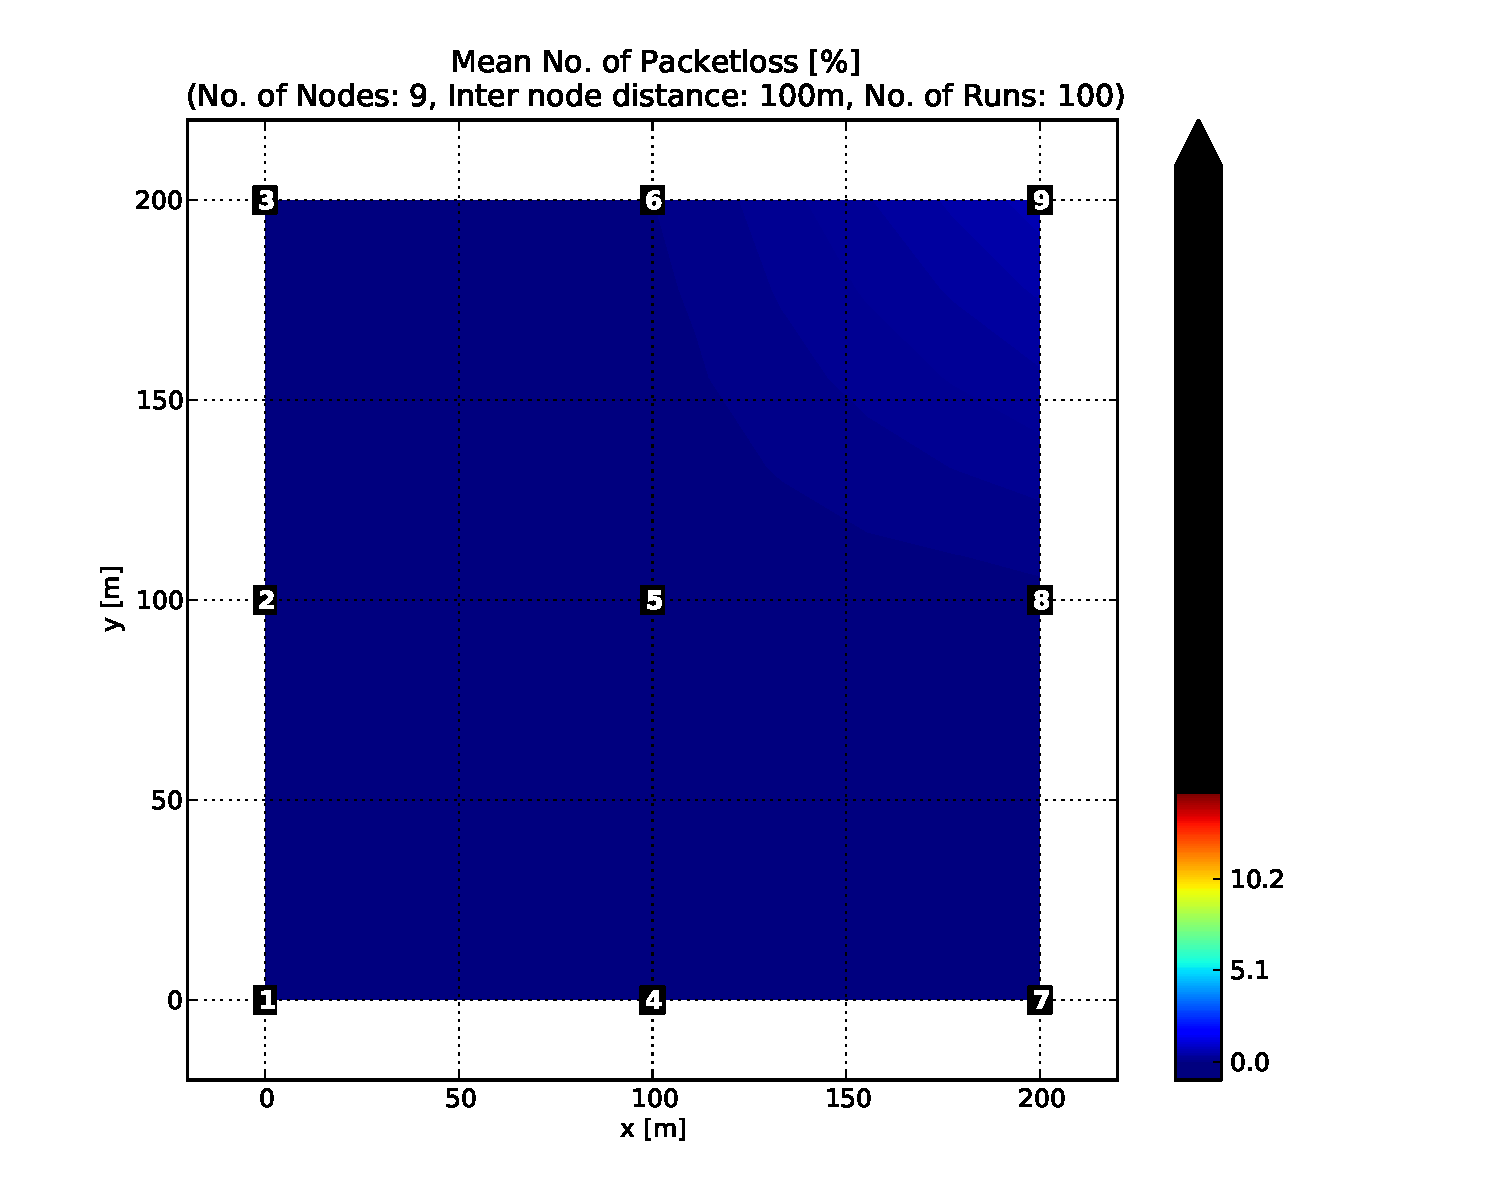
\includegraphics[trim=1.7cm 0cm 3cm 0cm, clip=true, scale=0.3]{Pics/results/9/OF0/grid/dist100_montecarlo_contour_packetloss.pdf}}
     \hspace{15pt}
    \subfloat[MRHOF]{\label{fig:9/MRHOF/grid/dist100_montecarlo_contour_packetloss}
     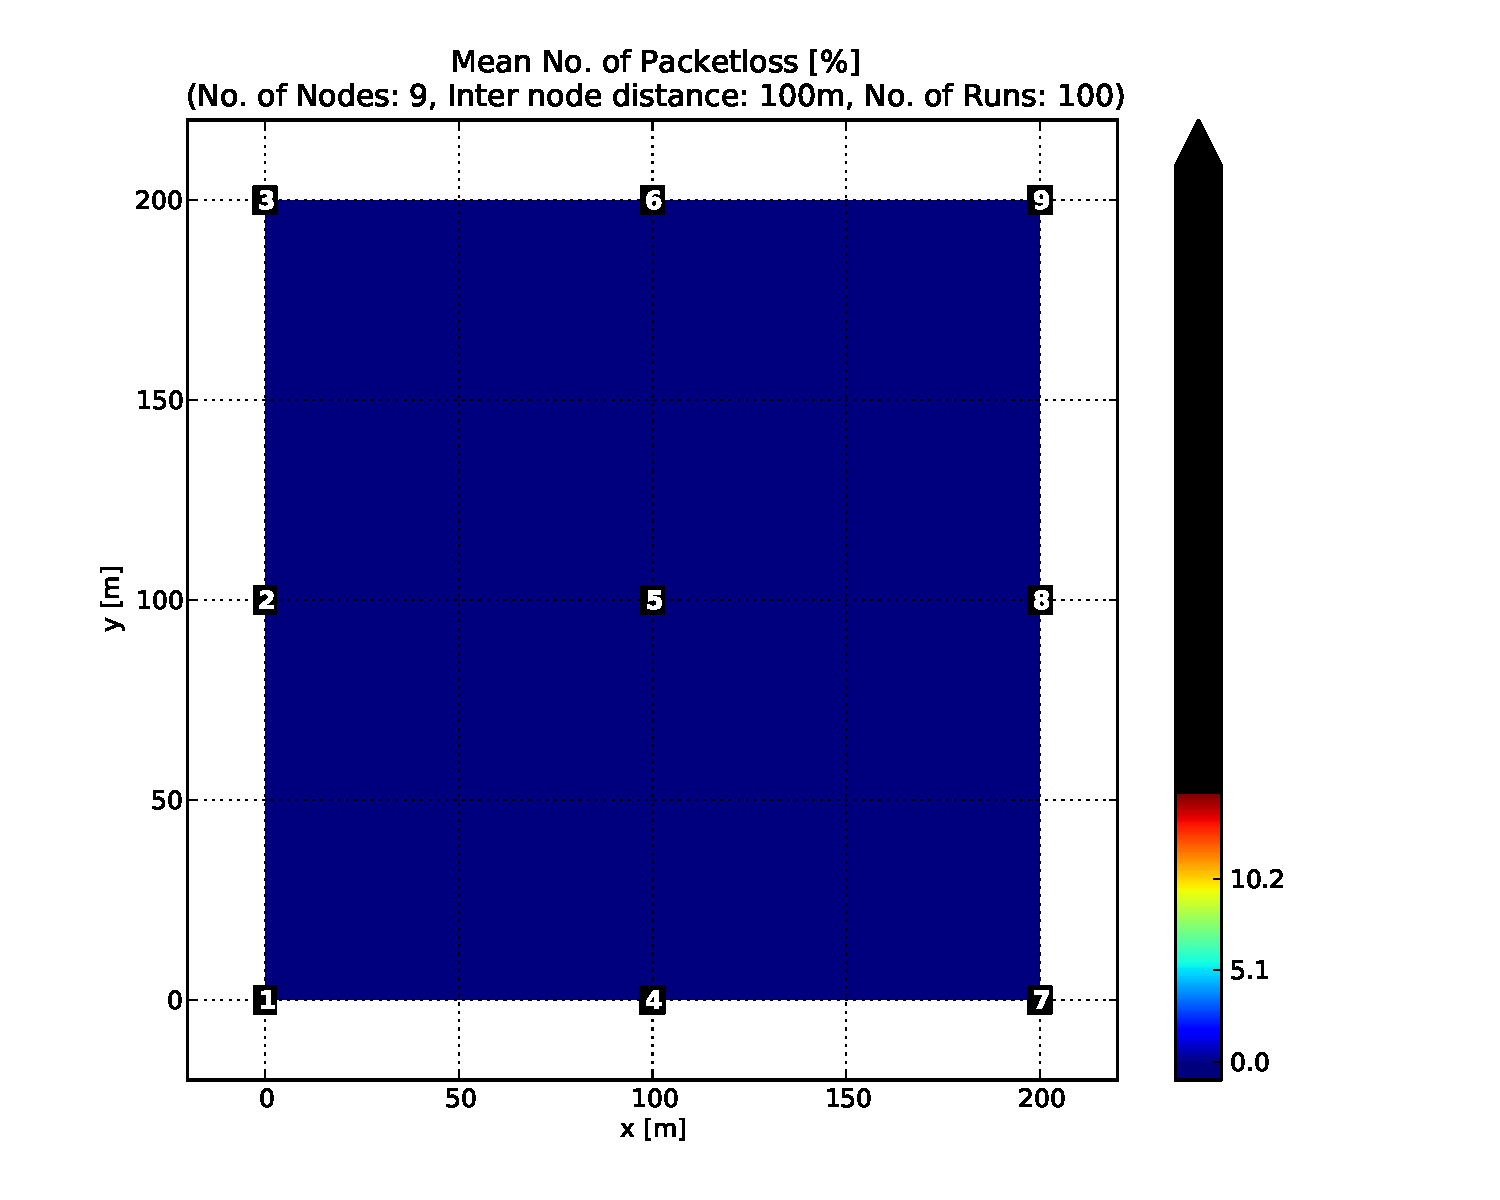
\includegraphics[trim=1.7cm 0cm 3cm 0cm, clip=true, scale=0.3]{Pics/results/9/MRHOF/grid/dist100_montecarlo_contour_packetloss.pdf}}
  \caption{Mean packet loss rate: 9-node grid scenario with 100~m inter-node distance}
  \label{fig:pl_9_grid_100}
   \vspace{-25pt}
\end{figure}

%%%%%%%%%%%%%%%%%%%%%%%%%%%%%%%%%%%%%%% grid 16 %%%%%%%%%%%%%%%%%%%%%%%%%%%%%%%%%%%%%%%%

\begin{figure}[p]
  \centering
   \vspace{-20pt}
    \leavevmode
    \subfloat[OF0]{\label{fig:16/OF0/grid/dist10_montecarlo_contour_packetloss}
      \includegraphics[trim=1.7cm 0cm 3cm 0cm, clip=true, scale=0.3]{Pics/results/16/OF0/grid/dist10_montecarlo_contour_packetloss.pdf}}
      \hspace{15pt}
    \subfloat[MRHOF]{\label{fig:16/MRHOF/grid/dist10_montecarlo_contour_packetloss}
      \includegraphics[trim=1.7cm 0cm 3cm 0cm, clip=true, scale=0.3]{Pics/results/16/MRHOF/grid/dist10_montecarlo_contour_packetloss.pdf}}
   \caption{Mean packet loss rate: 16-node grid scenario with 10~m inter-node distance}
   \label{fig:pl_16_grid_10}
    \vspace{-25pt}
\end{figure}

\begin{figure}[p]
  \centering
    \leavevmode
    \subfloat[OF0]{\label{fig:16/OF0/grid/dist50_montecarlo_contour_packetloss}
    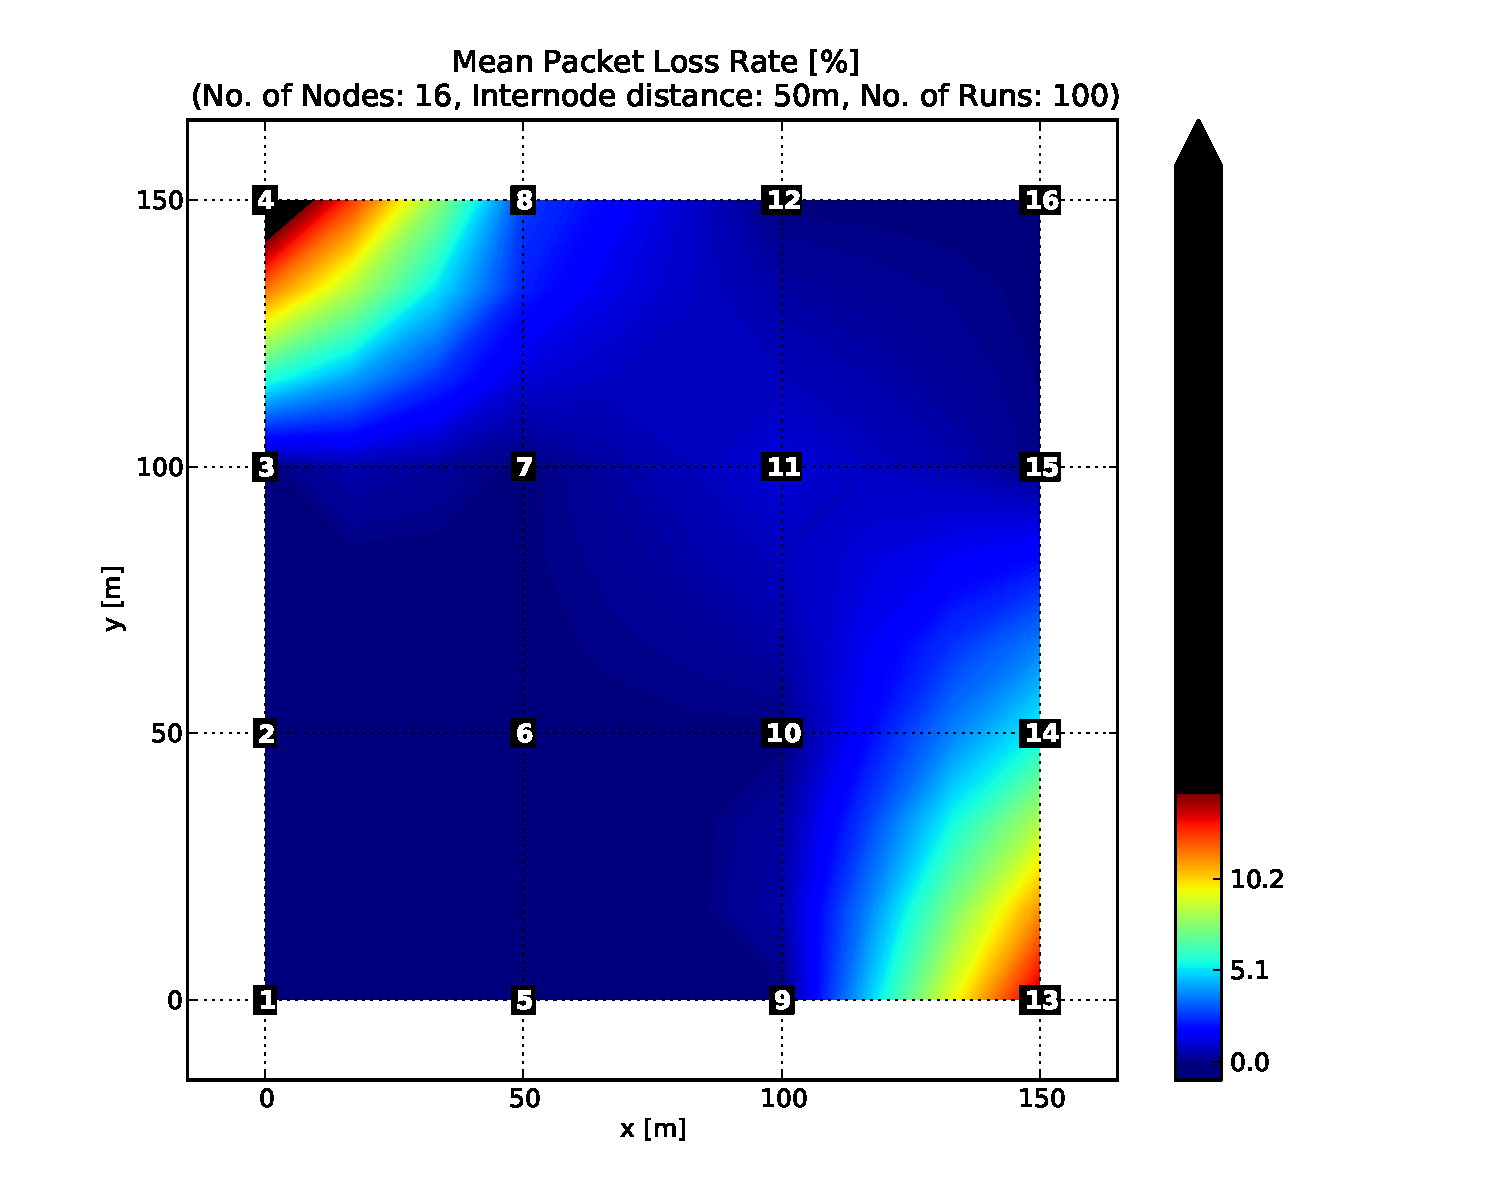
\includegraphics[trim=1.7cm 0cm 3cm 0cm, clip=true, scale=0.3]   {Pics/results/16/OF0/grid/dist50_montecarlo_contour_packetloss.pdf}}
    \hspace{15pt}
    \subfloat[MRHOF]{\label{fig:16/MRHOF/grid/dist50_montecarlo_contour_packetloss}
      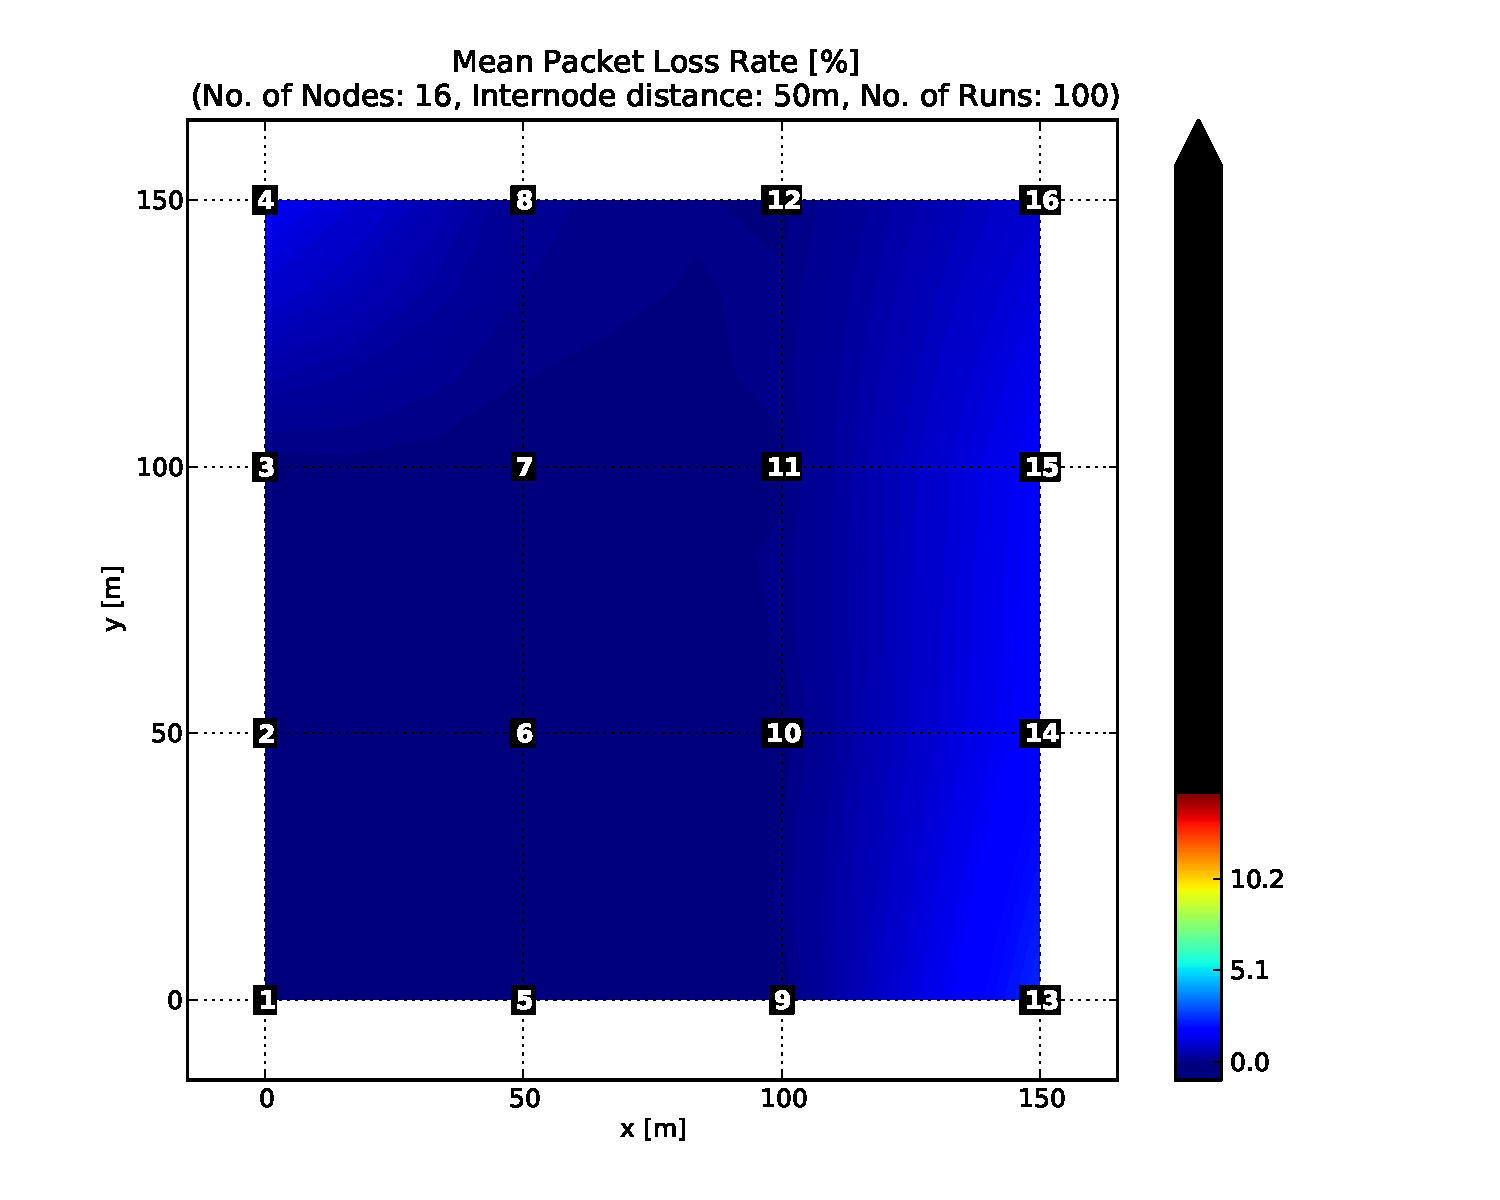
\includegraphics[trim=1.7cm 0cm 3cm 0cm, clip=true, scale=0.3]{Pics/results/16/MRHOF/grid/dist50_montecarlo_contour_packetloss.pdf}}
   \caption{Mean packet loss rate: 16-node grid scenario with 50~m inter-node distance}
   \label{fig:pl_16_grid_50}
    \vspace{-25pt}
\end{figure}

\begin{figure}[p]
  \centering
    \leavevmode
    \subfloat[OF0]{\label{fig:16/OF0/grid/dist100_montecarlo_contour_packetloss}
     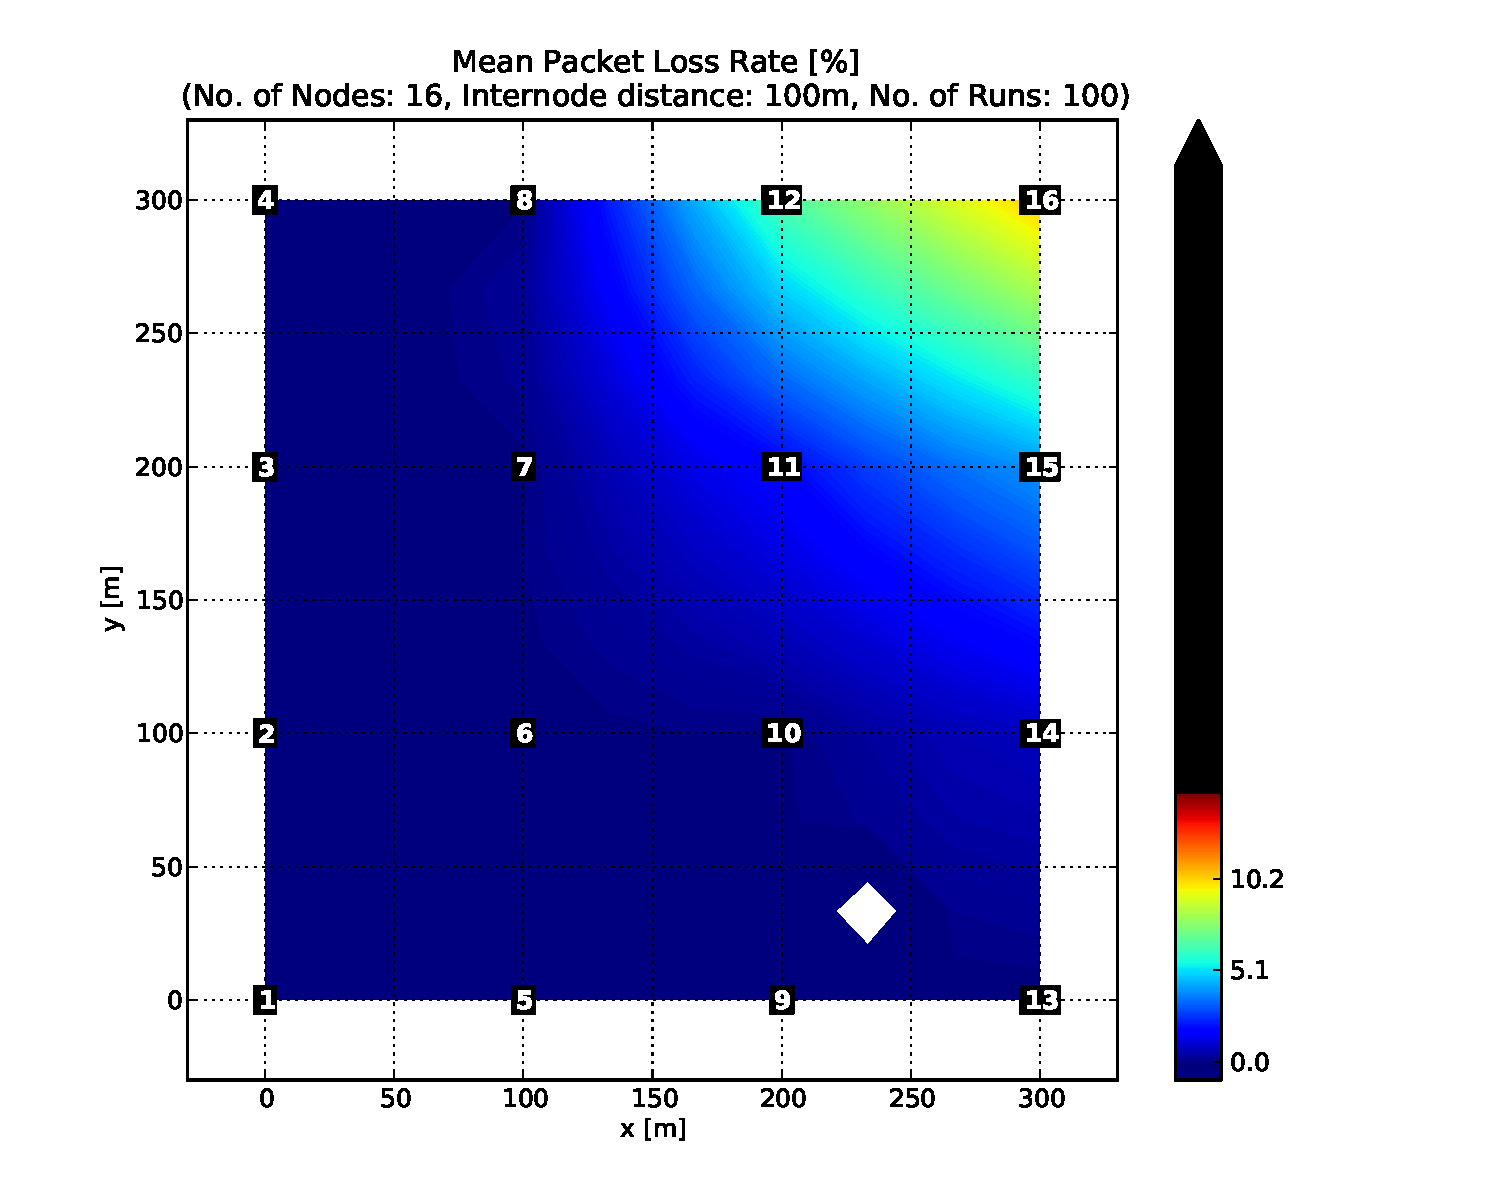
\includegraphics[trim=1.7cm 0cm 3cm 0cm, clip=true, scale=0.3]{Pics/results/16/OF0/grid/dist100_montecarlo_contour_packetloss.pdf}}
     \hspace{15pt}
    \subfloat[MRHOF]{\label{fig:16/MRHOF/grid/dist100_montecarlo_contour_packetloss}
     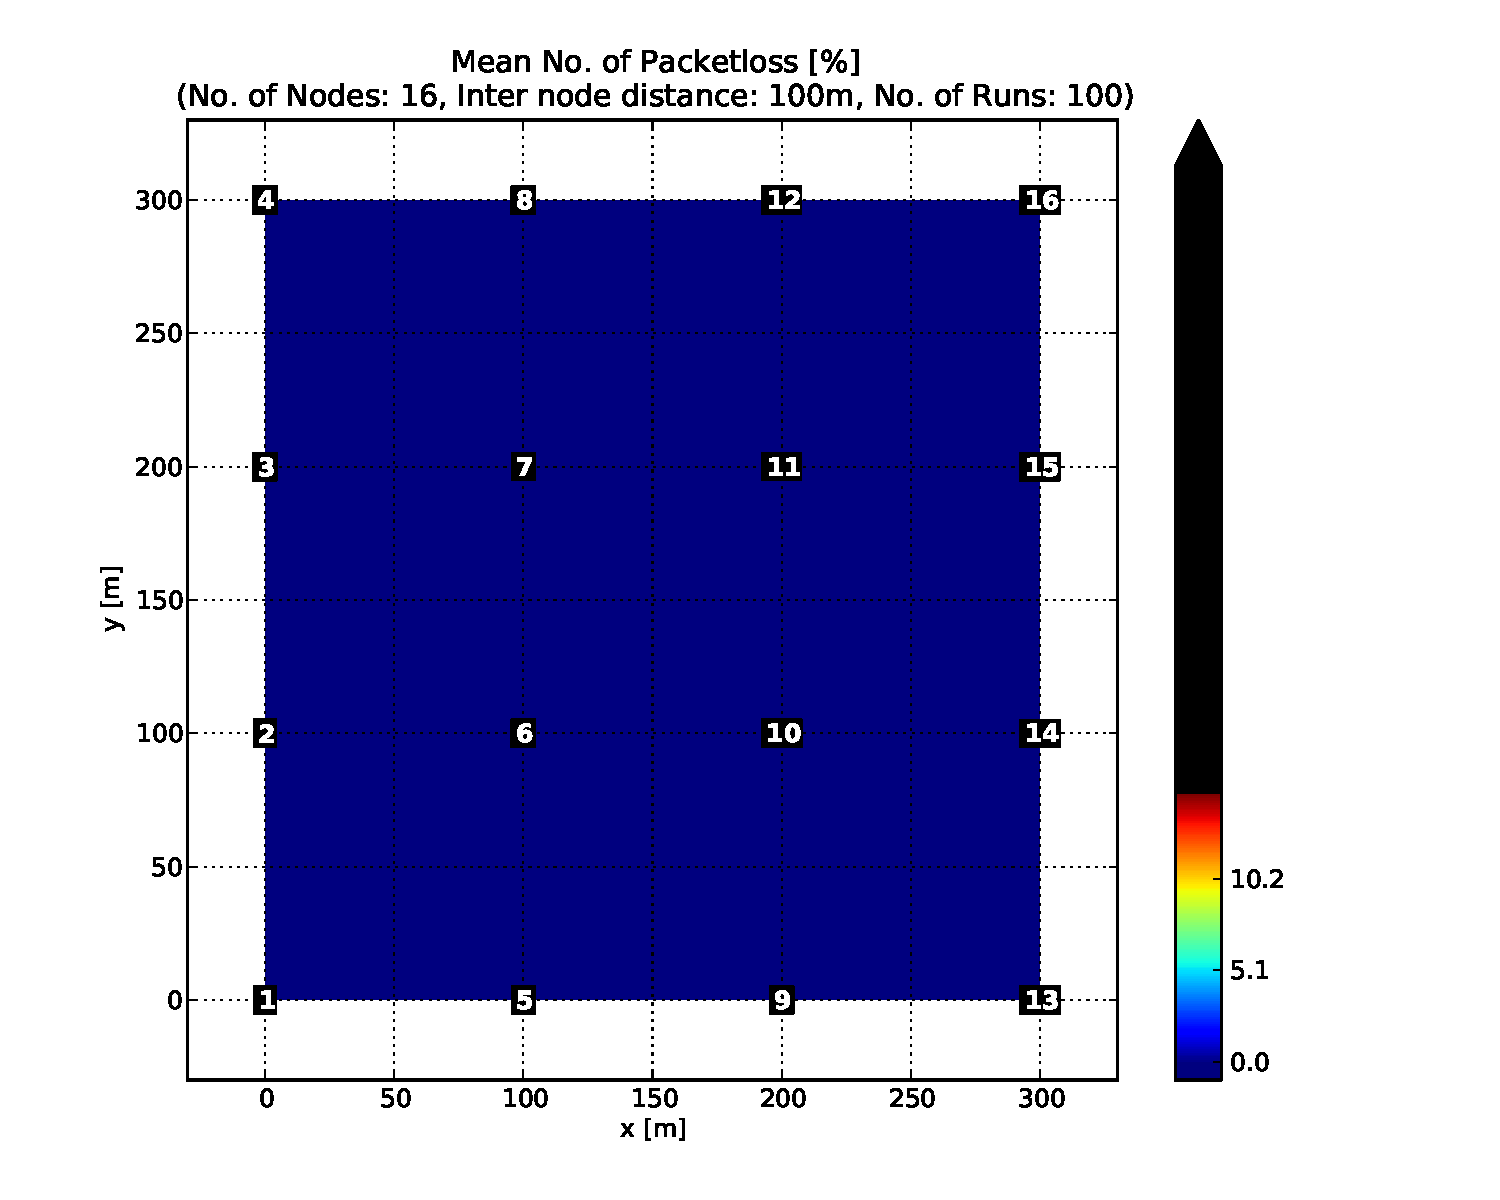
\includegraphics[trim=1.7cm 0cm 3cm 0cm, clip=true, scale=0.3]{Pics/results/16/MRHOF/grid/dist100_montecarlo_contour_packetloss.pdf}}
  \caption{Mean packet loss rate: 16-node grid scenario with 100~m inter-node distance}
  \label{fig:pl_16_grid_100}
   \vspace{-25pt}
\end{figure}
%%%%%%%%%%%%%%%%%%%%%%%%%%%%%%%%%%% RTT %%%%%%%%%%%%%%%%%%%%%%%%%%%%%%%%
\clearpage
\section{Round-Trip Time}
\label{rtt}

\subsection{Line Scenario}
\label{rtt:line}

The mean RTT for various node numbers and inter-node distances of the line scenario is shown in Figure~\ref{fig:rtt_4_line_10} to Figure~\ref{fig:rtt_16_line_100}. Again, the left side figures show the mean RTT results with OF0, and the right ones show the results for MRHOF.

Due to the PRR drops as the inter-node distance increases, the link quality between two nodes becomes bad, and packets cannot reach the destination within one hop. Therefore RPL forms routes for multi-hop delivery. This multi-hop delivery can be clearly seen by comparing the results of the 9-node line scenario. When the inter-node distance is 10~m (Figure~\ref{fig:9/OF0/line/dist10_montecarlo_contour}), node 9 is one hop away from the root, and has a mean RTT of 11~ms.  When the inter-node distance increases to 50~m (Figure~\ref{fig:9/OF0/line/dist50_montecarlo_contour}), node 9 is at least three hops away from the root, and has a mean RTT of 56~ms.  When the inter-node distance continues to increase to 100~m, node 9 becomes eight hops away, and the mean RTT for node 9 becomes 101~ms.  The phenomenon of increasing mean RTT with distance can be observed in the 4- and 16-node scenarios as well. For the line scenario, there is no apparent difference between OF0 and MRHOF in terms of increasement of mean RTT over inter-node distance. For both OFs under the same scenario setup, the mean RTT of the first hop is typically 11 ms, and each additional hop adds approximately 13~ms to it.

Similar to the mean packet loss rate results, the mean RTT performances of OF0 and MRHOF are different for the 16-node topology. In Figure~\ref{fig:16/OF0/line/dist50_montecarlo_contour} due to bad routes between the root and the most distant nodes, the mean RTT becomes higher than 250~ms while MRHOF keeps a mean RTT within 150~ms even for the furthest node.

\begin{figure}[p]
  \centering
    \leavevmode
    \subfloat[OF0]{\label{fig:4/OF0/line/dist10_montecarlo_contour}
      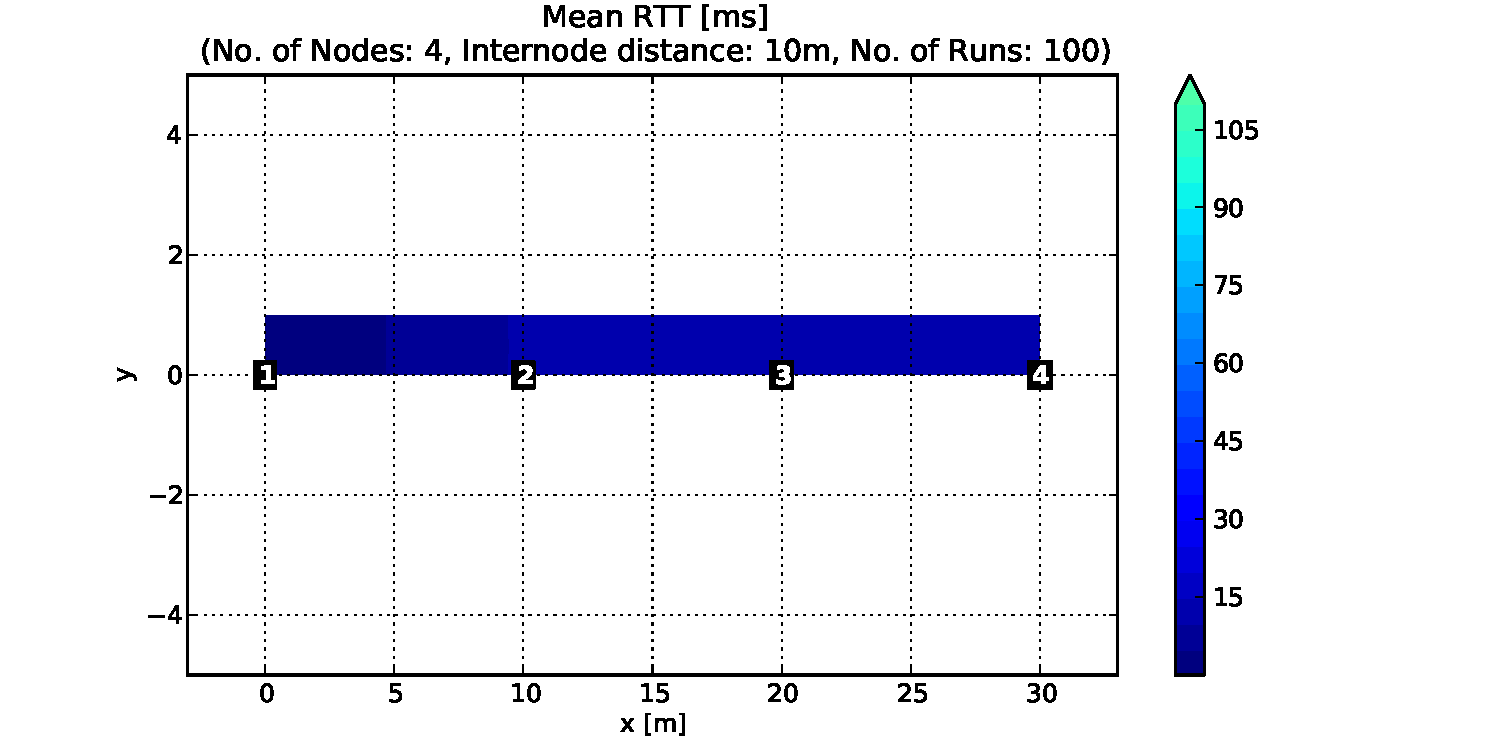
\includegraphics[trim=1.7cm 0cm 3cm 0cm, clip=true, scale=0.38]{Pics/results/4/OF0/line/dist10_montecarlo_contour.pdf}}
     \subfloat[MRHOF]{\label{fig:4/MRHOF/line/dist10_montecarlo_contour}
      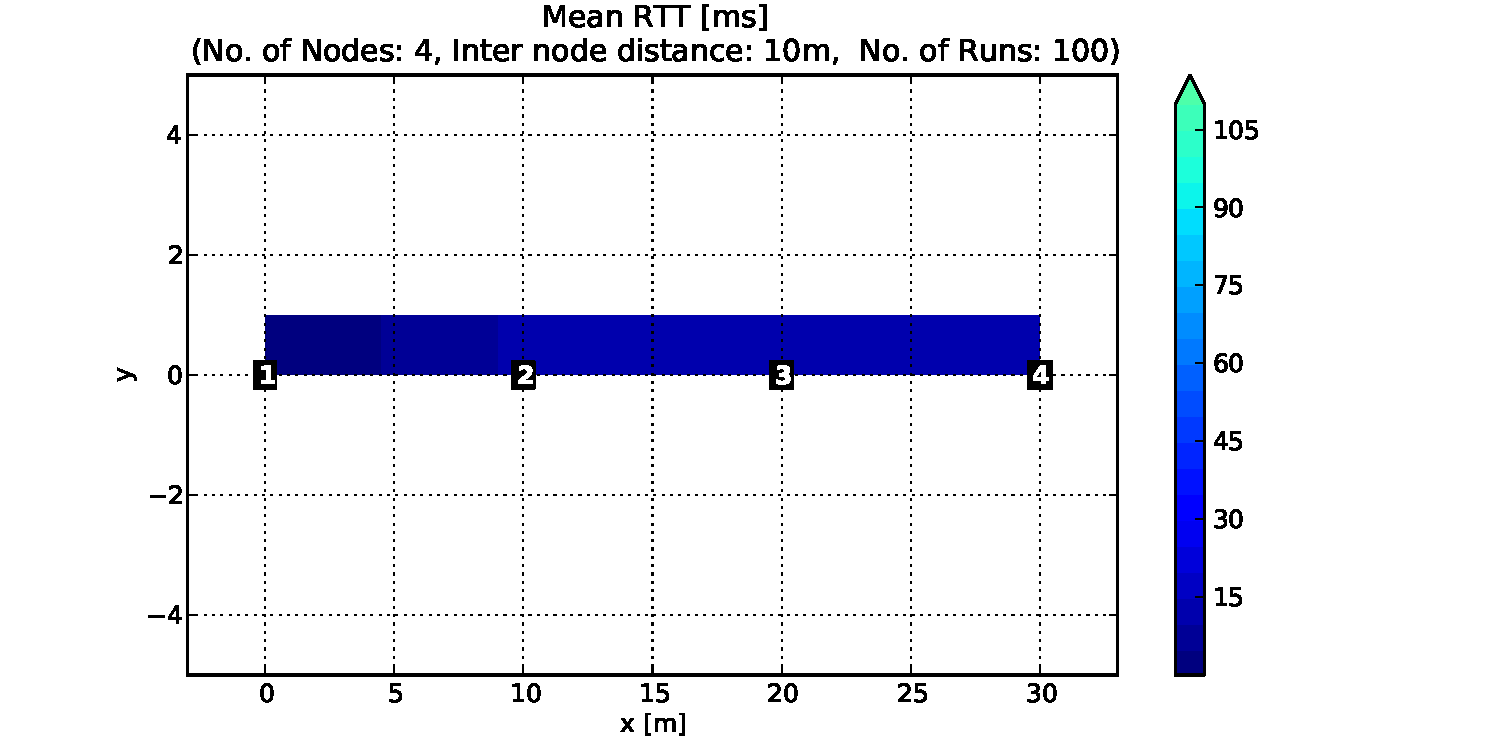
\includegraphics[trim=1.7cm 0cm 3cm 0cm, clip=true, scale=0.38]{Pics/results/4/MRHOF/line/dist10_montecarlo_contour.pdf}}
  \caption{Mean RTT: 4-node line scenario with 10~m inter-node distance}
 \label{fig:rtt_4_line_10}
\end{figure}

\begin{figure}[p]
  \centering
    \leavevmode
    \subfloat[OF0]{\label{fig:4/OF0/line/dist50_montecarlo_contour}
      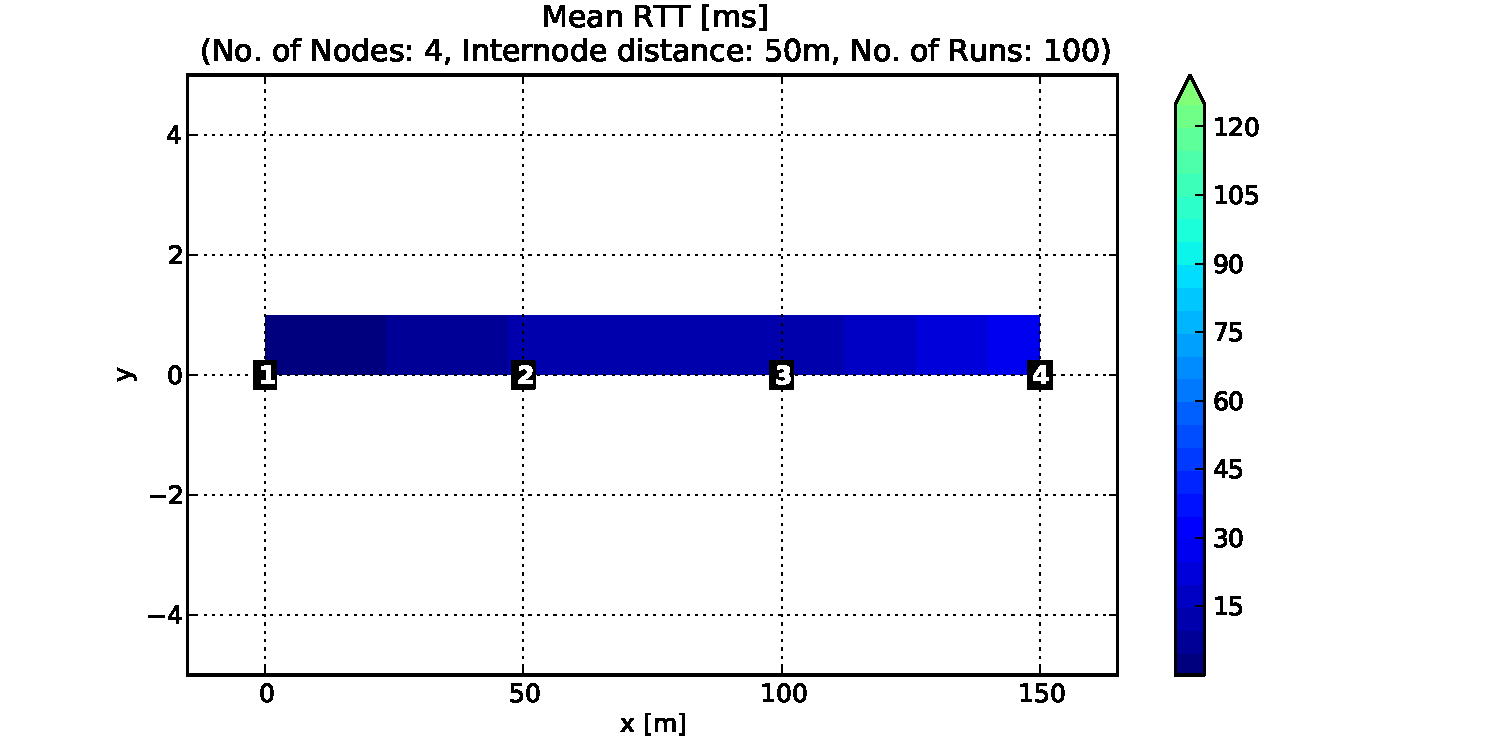
\includegraphics[trim=1.7cm 0cm 3cm 0cm, clip=true, scale=0.38]{Pics/results/4/OF0/line/dist50_montecarlo_contour.pdf}}
     \subfloat[MRHOF]{\label{fig:4/MRHOF/line/dist50_montecarlo_contour}
      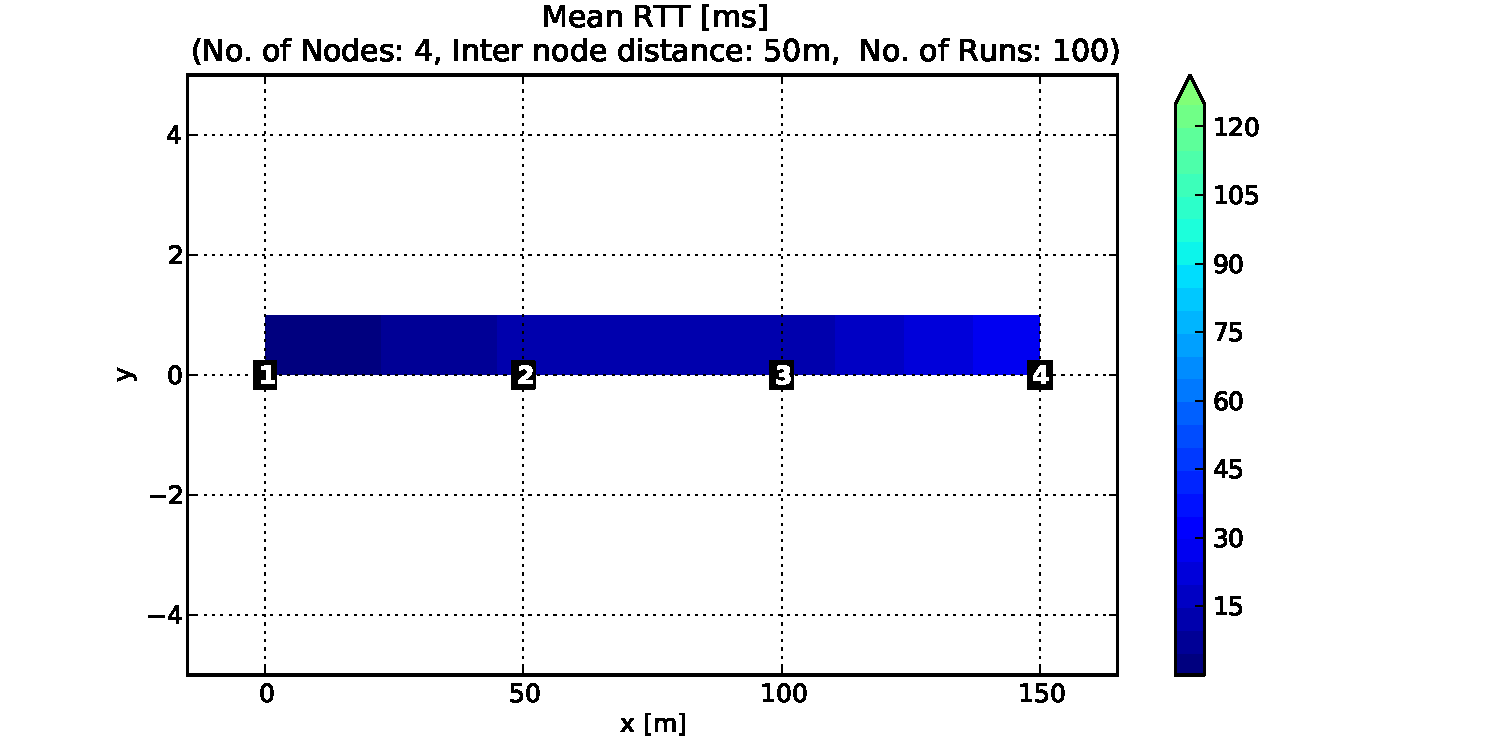
\includegraphics[trim=1.7cm 0cm 3cm 0cm, clip=true, scale=0.38]{Pics/results/4/MRHOF/line/dist50_montecarlo_contour.pdf}}
  \caption{Mean RTT: 4-node line scenario with 50~m inter-node distance}
 \label{fig:rtt_4_line_50}
\end{figure}

\begin{figure}[p]
  \centering
    \leavevmode
    \subfloat[OF0]{\label{fig:4/OF0/line/dist100_montecarlo_contour}
      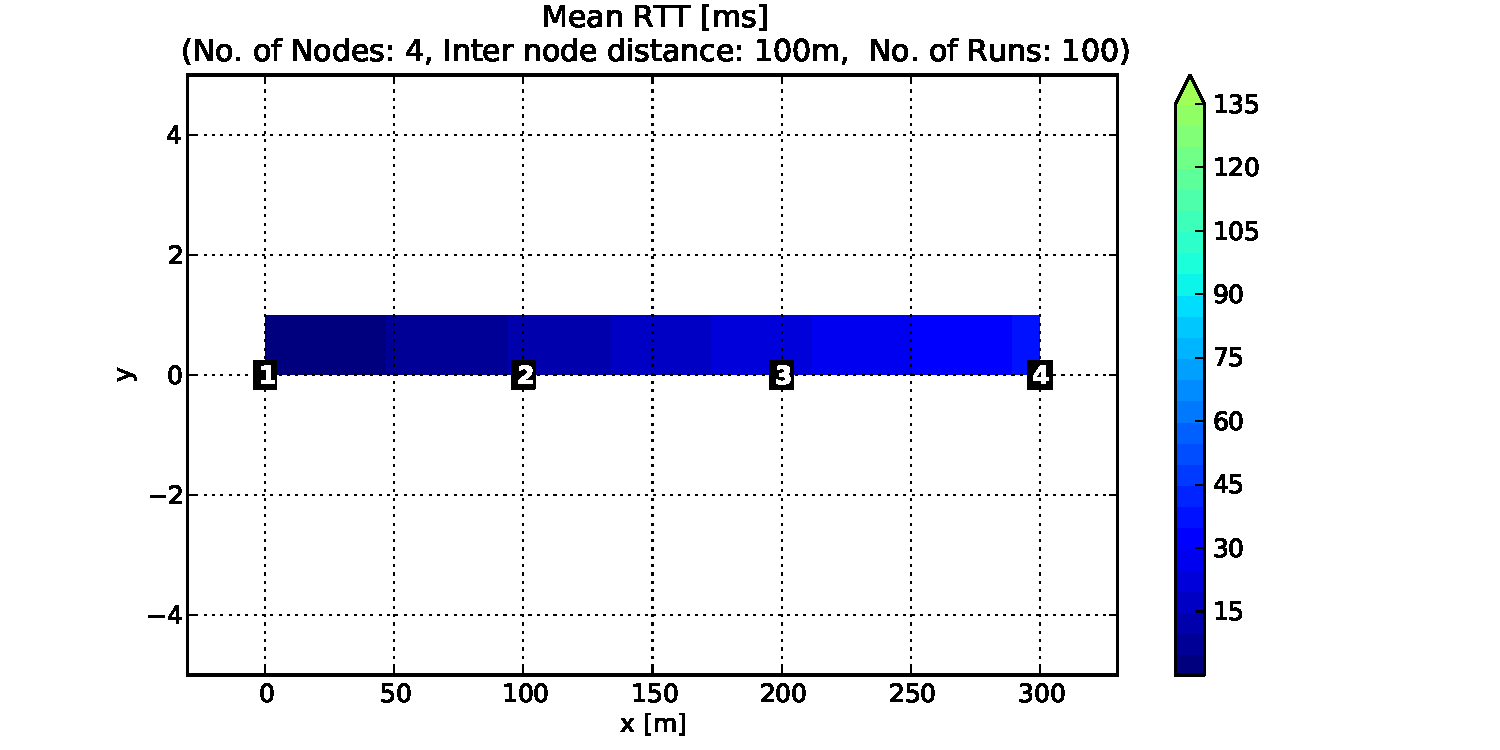
\includegraphics[trim=1.7cm 0cm 3cm 0cm, clip=true, scale=0.38]{Pics/results/4/OF0/line/dist100_montecarlo_contour.pdf}}
     \subfloat[MRHOF]{\label{fig:4/MRHOF/line/dist100_montecarlo_contour}
      \includegraphics[trim=1.7cm 0cm 3cm 0cm, clip=true, scale=0.38]{Pics/results/4/MRHOF/line/dist100_montecarlo_contour.pdf}}
  \caption{Mean RTT: 4-node line scenario with 100~m inter-node distance}
 \label{fig:rtt_4_line_100}
\end{figure}

%%%%%%%%%%%%%%%%%%%%%%%%%% line 9 %%%%%%%%%%%%%%%%%%%%%%%%%%%%%%%%%%%%%%%%%%%%%%%%%%%%%%

\begin{figure}[p]
  \centering
    \leavevmode
    \subfloat[OF0]{\label{fig:9/OF0/line/dist10_montecarlo_contour}
      \includegraphics[trim=1.7cm 0cm 3cm 0cm, clip=true, scale=0.38]{Pics/results/9/OF0/line/dist10_montecarlo_contour.pdf}}
     \subfloat[MRHOF]{\label{fig:9/MRHOF/line/dist10_montecarlo_contour}
      \includegraphics[trim=1.7cm 0cm 3cm 0cm, clip=true, scale=0.38]     {Pics/results/9/MRHOF/line/dist10_montecarlo_contour.pdf}}
  \caption{Mean RTT: 9-node line scenario with 10~m inter-node distance}
 \label{fig:rtt_9_line_10}
\end{figure}

\begin{figure}[p]
  \centering
    \leavevmode
    \subfloat[OF0]{\label{fig:9/OF0/line/dist50_montecarlo_contour}
      \includegraphics[trim=1.7cm 0cm 3cm 0cm, clip=true, scale=0.38]{Pics/results/9/OF0/line/dist50_montecarlo_contour.pdf}}
     \subfloat[MRHOF]{\label{fig:9/MRHOF/line/dist50_montecarlo_contour}
      \includegraphics[trim=1.7cm 0cm 3cm 0cm, clip=true, scale=0.38]{Pics/results/9/MRHOF/line/dist50_montecarlo_contour.pdf}}
  \caption{Mean RTT: 9-node line scenario with 50~m inter-node distance}
 \label{fig:rtt_9_line_50}
\end{figure}

\begin{figure}[p]
  \centering
    \leavevmode
    \subfloat[OF0]{\label{fig:9/OF0/line/dist100_montecarlo_contour}
      \includegraphics[trim=1.7cm 0cm 3cm 0cm, clip=true, scale=0.38]{Pics/results/9/OF0/line/dist100_montecarlo_contour.pdf}}
     \subfloat[MRHOF]{\label{fig:9/MRHOF/line/dist100_montecarlo_contour}
      \includegraphics[trim=1.7cm 0cm 3cm 0cm, clip=true, scale=0.38]{Pics/results/9/MRHOF/line/dist100_montecarlo_contour.pdf}}
  \caption{Mean RTT: 9-node line scenario with 100~m inter-node distance}
 \label{fig:rtt__line_100}
\end{figure}

%%%%%%%%%%%%%%%%%%%%%%%%%%%%%%%%%% line 16 %%%%%%%%%%%%%%%%%%%%%%%%%%%%%%%%%%%%%%

\begin{figure}[p]
  \centering
    \leavevmode
    \subfloat[OF0]{\label{fig:16/OF0/line/dist10_montecarlo_contour}
      \includegraphics[trim=1.7cm 0cm 3cm 0cm, clip=true, scale=0.38]{Pics/results/16/OF0/line/dist10_montecarlo_contour.pdf}}
     \subfloat[MRHOF]{\label{fig:16/MRHOF/line/dist10_montecarlo_contour}
      \includegraphics[trim=1.7cm 0cm 3cm 0cm, clip=true, scale=0.38]{Pics/results/16/MRHOF/line/dist10_montecarlo_contour.pdf}}
  \caption{Mean RTT: 16-node line scenario with 10~m inter-node distance}
 \label{fig:rtt_16_line_10}
\end{figure}

\begin{figure}[p]
  \centering
    \leavevmode
    \subfloat[OF0]{\label{fig:16/OF0/line/dist50_montecarlo_contour}
      \includegraphics[trim=1.7cm 0cm 3cm 0cm, clip=true, scale=0.38]{Pics/results/16/OF0/line/dist50_montecarlo_contour.pdf}}
     \subfloat[MRHOF]{\label{fig:16/MRHOF/line/dist50_montecarlo_contour}
      \includegraphics[trim=1.7cm 0cm 3cm 0cm, clip=true, scale=0.38]{Pics/results/16/MRHOF/line/dist50_montecarlo_contour.pdf}}
  \caption{Mean RTT: 16-node line scenario with 50~m inter-node distance}
 \label{fig:rtt_16_line_50}
\end{figure}

\begin{figure}[p]
  \centering
    \leavevmode
    \subfloat[OF0]{\label{fig:16/OF0/line/dist100_montecarlo_contour}
      \includegraphics[trim=1.7cm 0cm 3cm 0cm, clip=true, scale=0.38] {Pics/results/16/OF0/line/dist100_montecarlo_contour.pdf}}
     \subfloat[MRHOF]{\label{fig:16/MRHOF/line/dist100_montecarlo_contour}
      \includegraphics[trim=1.7cm 0cm 3cm 0cm, clip=true, scale=0.38]{Pics/results/16/MRHOF/line/dist100_montecarlo_contour.pdf}}
  \caption{Mean RTT: 16-node line scenario with 100~m inter-node distance}
 \label{fig:rtt_16_line_100}
\end{figure}


\clearpage
\subsection{Grid Scenario}
\label{rtt:grid}

Figure~\ref{fig:rtt_4_grid_10} to Figure~\ref{fig:rtt_16_grid_100} illustrate the mean RTT results of the grid scenario simulations. The phenomenon of increasing mean RTT with inter-node distance (mentioned in Section \ref{rtt:line}) can be observed here again. In Figure~\ref{fig:4/OF0/grid/dist50_montecarlo_contour} and Figure~\ref{fig:4/OF0/grid/dist100_montecarlo_contour}, one can see the mean RTT increasement with distance of a 4-node grid scenario using OF0. The mean RTT for node 4 increases from  10.7~ms to 73.8~ms while the inter-node distance increases from 50~m to 100~m. Similarly, in Figure~\ref{fig:4/MRHOF/grid/dist50_montecarlo_contour} and Figure~\ref{fig:4/MRHOF/grid/dist100_montecarlo_contour}, by using MRHOF the mean RTT for node 4 increases from  11.1~ms to 69.4~ms while the inter-node distance increases from 50~m to 100~m.

When the node number increases, the difference between OF0 and MRHOF in terms of mean RTT increasement over distance grows bigger. For the 9-node grid scenario with OF0, the mean RTT of node 9 increases from 72.5~ms (inter-node distance 50~m, Figure~\ref{fig:9/OF0/grid/dist50_montecarlo_contour}) to 142.1~ms (inter-node distance 100~m, Figure~\ref{fig:9/OF0/grid/dist100_montecarlo_contour}) while with MRHOF it increases from 68.2~ms (inter-node distance 50~m, Figure~\ref{fig:9/MRHOF/grid/dist50_montecarlo_contour}) to 79.9~ms (inter-node distance 100~m, Figure~\ref{fig:9/MRHOF/grid/dist100_montecarlo_contour}). For the 16-node grid scenario using OF0, the mean RTT of node 16 increases from 35.1~ms (inter-node distance 50~m, Figure~\ref{fig:16/OF0/grid/dist50_montecarlo_contour}) to infinite (inter-node distance 100~m, Figure~\ref{fig:9/OF0/grid/dist100_montecarlo_contour}) due to bad route between the root and node 16 in one or more runs. On the other hand, with MRHOF the mean RTT of node 16 grows from 50.8~ms (inter-node distance 50~m, Figure~\ref{fig:16/MRHOF/grid/dist50_montecarlo_contour}) to 116.0~ms (inter-node distance 100~m, Figure~\ref{fig:16/MRHOF/grid/dist100_montecarlo_contour}). Moreover, in Figure~\ref{fig:16/OF0/grid/dist50_montecarlo_contour} and Figure~\ref{fig:16/OF0/grid/dist100_montecarlo_contour}, one can see the instances of broken routes between the root and the nodes happened again for the 16-node grid scenario with 50 or 100~m inter-node distance.

By comparing the mean RTT results of OF0 and MRHOF, one can say that in terms of mean RTT MRHOF has a better performance than OF0 for the nodes which are more than one hop away.

%\clearpage
\begin{figure}[p]
  \centering
  \vspace{-20pt}
    \leavevmode
    \subfloat[OF0]{\label{fig:4/OF0/grid/dist10_montecarlo_contour}
      \includegraphics[trim=1cm 0cm 3cm 0cm, clip=true, scale=0.3]{Pics/results/4/OF0/grid/dist10_montecarlo_contour.pdf}} 
      \hspace{15pt}
     \subfloat[MRHOF]{\label{fig:4/MRHOF/grid/dist10_montecarlo_contour}
      \includegraphics[trim=1cm 0cm 3cm 0cm, clip=true, scale=0.3]{Pics/results/4/MRHOF/grid/dist10_montecarlo_contour.pdf}}
  \caption{Mean RTT: 4-node grid scenario with 10~m inter-node distance}
 \label{fig:rtt_4_grid_10}
 \vspace{-25pt}
\end{figure}

\begin{figure}[p]
  \centering
    \leavevmode
    \subfloat[OF0]{\label{fig:4/OF0/grid/dist50_montecarlo_contour}
      \includegraphics[trim=1cm 0cm 3cm 0cm, clip=true, scale=0.3]{Pics/results/4/OF0/grid/dist50_montecarlo_contour.pdf}} 
      \hspace{15pt}
     \subfloat[MRHOF]{\label{fig:4/MRHOF/grid/dist50_montecarlo_contour}
      \includegraphics[trim=1cm 0cm 3cm 0cm, clip=true, scale=0.3]{Pics/results/4/MRHOF/grid/dist50_montecarlo_contour.pdf}}
  \caption{Mean RTT: 4-node grid scenario with 50~m inter-node distance}
 \label{fig:rtt_4_grid_50}
 \vspace{-25pt}
\end{figure}

\begin{figure}[p]
  \centering
    \leavevmode
    \subfloat[OF0]{\label{fig:4/OF0/grid/dist100_montecarlo_contour}
      \includegraphics[trim=1cm 0cm 3cm 0cm, clip=true, scale=0.3]
      {Pics/results/4/OF0/grid/dist100_montecarlo_contour.pdf}} 
      \hspace{15pt}
     \subfloat[MRHOF]{\label{fig:4/MRHOF/grid/dist100_montecarlo_contour}
      \includegraphics[trim=1cm 0cm 3cm 0cm, clip=true, scale=0.3]
      {Pics/results/4/MRHOF/grid/dist100_montecarlo_contour.pdf}}
  \caption{Mean RTT: 4-node grid scenario with 100~m inter-node distance}
 \label{fig:rtt_4_grid_100}
 \vspace{-25pt}
\end{figure}

%%%%%%%%%%%%%%%%%%%%%%%%%% grid 9 %%%%%%%%%%%%%%%%%%%%%%%%%%%%%%%%%%%%%%%%%%%%%%%%%%%%%%

\begin{figure}[p]
  \centering
   \vspace{-20pt}
    \leavevmode
    \subfloat[OF0]{\label{fig:9/OF0/grid/dist10_montecarlo_contour}
      \includegraphics[trim=1cm 0cm 3cm 0cm, clip=true, scale=0.3]
      {Pics/results/9/OF0/grid/dist10_montecarlo_contour.pdf}} 
      \hspace{15pt}
     \subfloat[MRHOF]{\label{fig:9/MRHOF/grid/dist10_montecarlo_contour}
      \includegraphics[trim=1cm 0cm 3cm 0cm, clip=true, scale=0.3]
      {Pics/results/9/MRHOF/grid/dist10_montecarlo_contour.pdf}}
  \caption{Mean RTT: 9-node grid scenario with 10~m inter-node distance}
 \label{fig:rtt_9_grid_10}
 \vspace{-25pt}
\end{figure}

\begin{figure}[p]
  \centering
    \leavevmode
    \subfloat[OF0]{\label{fig:9/OF0/grid/dist50_montecarlo_contour}
      \includegraphics[trim=1cm 0cm 3cm 0cm, clip=true, scale=0.3]{Pics/results/9/OF0/grid/dist50_montecarlo_contour.pdf}} 
      \hspace{15pt}
     \subfloat[MRHOF]{\label{fig:9/MRHOF/grid/dist50_montecarlo_contour}
      \includegraphics[trim=1cm 0cm 3cm 0cm, clip=true, scale=0.3]{Pics/results/9/MRHOF/grid/dist50_montecarlo_contour.pdf}}
  \caption{Mean RTT: 9-node grid scenario with 50~m inter-node distance}
 \label{fig:rtt_9_grid_50}
 \vspace{-25pt}
\end{figure}

\begin{figure}[p]
  \centering
    \leavevmode
    \subfloat[OF0]{\label{fig:9/OF0/grid/dist100_montecarlo_contour}
      \includegraphics[trim=1cm 0cm 3cm 0cm, clip=true, scale=0.3]{Pics/results/9/OF0/grid/dist100_montecarlo_contour.pdf}} 
      \hspace{15pt}
     \subfloat[MRHOF]{\label{fig:9/MRHOF/grid/dist100_montecarlo_contour}
      \includegraphics[trim=1cm 0cm 3cm 0cm, clip=true, scale=0.3]{Pics/results/9/MRHOF/grid/dist100_montecarlo_contour.pdf}}
  \caption{Mean RTT: 9-node grid scenario with 100~m inter-node distance}
 \label{fig:rtt__grid_100}
 \vspace{-25pt}
\end{figure}

%%%%%%%%%%%%%%%%%%%%%%%%%%%%%%%%%% grid 16 %%%%%%%%%%%%%%%%%%%%%%%%%%%%%%%%%%%%%%

\begin{figure}[p]
  \centering
  \vspace{-20pt}
    \leavevmode
    \subfloat[OF0]{\label{fig:16/OF0/grid/dist10_montecarlo_contour}
      \includegraphics[trim=1cm 0cm 3cm 0cm, clip=true, scale=0.3]{Pics/results/16/OF0/grid/dist10_montecarlo_contour.pdf}} 
      \hspace{15pt}
     \subfloat[MRHOF]{\label{fig:16/MRHOF/grid/dist10_montecarlo_contour}
      \includegraphics[trim=1cm 0cm 3cm 0cm, clip=true, scale=0.3]{Pics/results/16/MRHOF/grid/dist10_montecarlo_contour.pdf}}
  \caption{Mean RTT: 16-node grid scenario with 10~m inter-node distance}
 \label{fig:rtt_16_grid_10}
 \vspace{-25pt}
\end{figure}

\begin{figure}[p]
  \centering
    \leavevmode
    \subfloat[OF0]{\label{fig:16/OF0/grid/dist50_montecarlo_contour}
      \includegraphics[trim=1cm 0cm 3cm 0cm, clip=true, scale=0.3]{Pics/results/16/OF0/grid/dist50_montecarlo_contour.pdf}} 
      \hspace{15pt}
     \subfloat[MRHOF]{\label{fig:16/MRHOF/grid/dist50_montecarlo_contour}
      \includegraphics[trim=1cm 0cm 3cm 0cm, clip=true, scale=0.3]{Pics/results/16/MRHOF/grid/dist50_montecarlo_contour.pdf}}
  \caption{Mean RTT: 16-node grid scenario with 50~m inter-node distance}
 \label{fig:rtt_16_grid_50}
 \vspace{-25pt}
\end{figure}

\begin{figure}[p]
  \centering
    \leavevmode
    \subfloat[OF0]{\label{fig:16/OF0/grid/dist100_montecarlo_contour}
      \includegraphics[trim=1cm 0cm 3cm 0cm, clip=true, scale=0.3]{Pics/results/16/OF0/grid/dist100_montecarlo_contour.pdf}} 
      \hspace{15pt}
     \subfloat[MRHOF]{\label{fig:16/MRHOF/grid/dist100_montecarlo_contour}
      \includegraphics[trim=1cm 0cm 3cm 0cm, clip=true, scale=0.3]{Pics/results/16/MRHOF/grid/dist100_montecarlo_contour.pdf}}
  \caption{Mean RTT: 16-node grid scenario with 100~m inter-node distance}
 \label{fig:rtt_16_grid_100}
 \vspace{-25pt}
\end{figure}


%%%%%%%%%%%%%%%%%%%%%%%%%%%%%%%%%%%%%%%%%%%%%%%%%%%%%%%%%%%%%%%%%%%%%%%%%%%%%%%%%%%%%%%%%%%%%%%%%%%%%%%%%%%%%%




